\documentclass[a4paper,twoside,justified,notoc]{layout/fenicsbook}

% Book metadata
\title{Automated\\ \noindent Scientific\\ \noindent Computing}
\author[The FEniCS Project]{Logg, Mardal, Wells (Eds.)}
\publisher{Springer-Verlag}

% FIXME: Input package somewhere else
% Generate index
\usepackage{makeidx}
\makeindex

%------------------------------------------------------------------------------
% Begin document
\begin{document}

% Start front matter
\frontmatter

% Title page
\maketitle

% Copyright page
~\vfill
\thispagestyle{empty}
\setlength{\parindent}{0pt}
\setlength{\parskip}{\baselineskip}

%\par\smallcaps{Published by \thanklesspublisher}

\par
Copyright \copyright\ \the\year\ The FEniCS Project. \\
Permission is granted to copy, distribute and/or modify this document
under the terms of the GNU Free Documentation License, Version 1.3
or any later version published by the Free Software Foundation;
with no Invariant Sections, no Front-Cover Texts, and no Back-Cover Texts.
A copy of the license is included in the chapter entitled "GNU
Free Documentation License".
\index{license}

\par\textit{First printing, \monthyear}


% Contents
\tableofcontents
%\listoffigures
%\listoftables

%------------------------------------------------------------------------------
% Start main matter
\mainmatter

% Start full width
\begin{fullwidth}

% Chapters

%------------------------------------------------------------------------------

% Use to test individual chapter
%\fenicsinput{langtangen}\end{fullwidth}\end{document}

%\fenicschapter{Introduction}
              {Introduction}
              {Anders Logg, Garth N. Wells and Kent-Andre Mardal}
              {intro}

%\fenicsinput{langtangen}
%
%\part{Methodology}
%
%\fenicsinput{kirby-7}
%\fenicsinput{kirby-6}
%\fenicsinput{kirby-1}
%\fenicsinput{kirby-5}
%\fenicsinput{logg-3}
%\fenicsinput{oelgaard-2}
%\fenicsinput{kirby-8}
%\fenicsinput{kirby-4}
%%%%\fenicsinput{hoffman-4}
%
%\part{Implementation}
%
%%%%\fenicsinput{logg-2}
%\fenicsinput{logg-1}
%\fenicsinput{kirby-3}
%\fenicsinput{kirby-2}
%\fenicsinput{wilbers}
%\fenicsinput{alnes-3}
%\fenicsinput{alnes-2}
%\fenicsinput{alnes-1}
%%\fenicschapter{Unicorn: A Unified Continuum Mechanics Solver}
              {Unicorn: A Unified Continuum Mechanics Solver}
              {Cem Degirmenci, Johan Hoffman, Johan Jansson, Niclas Jansson and Murtazo Nazarov}
              {hoffman-2}

This chapter provides a description of the technology
in Unicorn focusing on simple, efficient and general
algorithms and software implementation of the Unified
Continuum (UC) concept and the adaptive General
Galerkin (G2) discretization as a unified approach to
continuum mechanics. We describe how Unicorn fits into
the FEniCS framework, how it interfaces to other
FEniCS components and what interfaces and
functionality Unicorn provides itself and how the
implementation is designed. We also give use case
application examples in fluid-structure interaction
and adaptivity.

For a more detailed discussion on turbulence and adaptive error
control in continuum mechanics we refer to
chapter \ref{chap:hoffman-1}.

\index{unicorn}

\section{Background}

Unicorn is solver technology (models, methods, algorithms and software
implementations) with the goal of automated simulation of realistic
continuum mechanics applications, such as drag or lift computation for
fixed or flexible objects (fluid-structure interaction) in turbulent
incompressible or compressible flow (airplane or bird flight, car
aerodynamics). The basis for Unicorn is Unified Continuum (UC)
modeling formulated in Euler (laboratory) coordinates, together with a
G2 (General Galerkin) adaptive stabilized FEM discretization with a
moving mesh for tracking the phase interfaces. The UC model consists
of canonical conservation equations for mass, momentum, energy and
phase over the whole domain as one continuum, together with a Cauchy
stress and phase variable as data for defining material properties and
constitutive equation. Unicorn formulates and implements the adaptive
G2 method applied to the UC model, and interfaces to other components
in the FEniCS chain (FIAT, FFC, DOLFIN) providing representation of
finite element function spaces, weak forms and mesh, and algorithms
such as automated parallel assembly and linear algebra.

Unicorn as part of the FEniCS framework realizes automated
computational modeling for general continuum mechanics applications in
the form of canonical UC formulation in Euler coordinates,
duality-based adaptive error control, tensor assembly, time-stepping,
adaptive fixed-point iteration for solving discrete systems, mesh
adaptivity by local cell operations (split, collapse, swap) (through
MAdLib) and cell quality optimization (smoothing).

% Comment out until persistent URL can be found
%A live CD with snapshots of Unicorn corresponding to the Unicorn
%chapters in this book is available
%at: \url{ftp://ftp.nada.kth.se/local/jjan/unicorn_fenics-book.iso}.

\begin{figure}[!h]
\center{
\boxed{
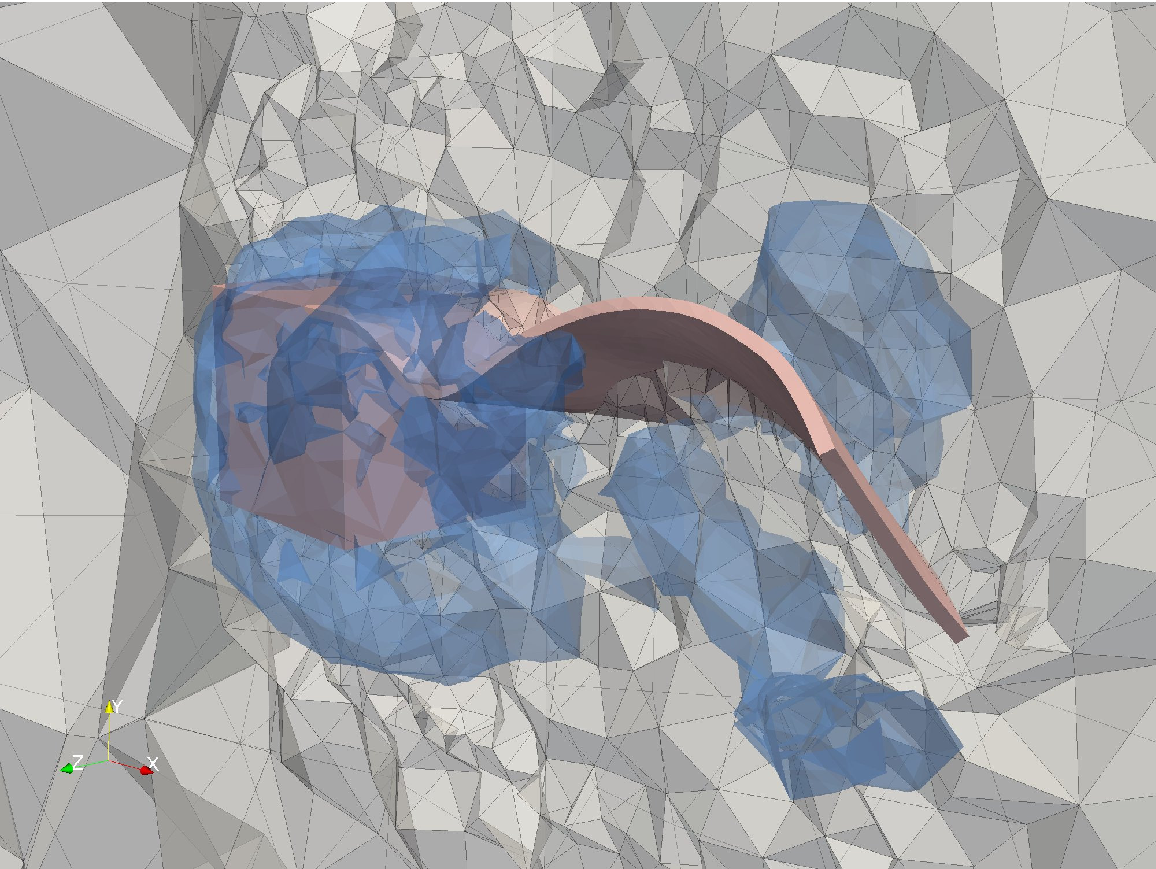
\includegraphics[width=10cm]{unfinished/hoffman-2/pdf/cube556.pdf}
}}
%\includegraphics[width=10cm]{media/unicorn_fsi_flag3D_01.pdf}
\caption{
A fluid-structure example application of a flag mounted behind a cube in turbulent flow. The fluid-structure interface, an isosurface of the pressure and a cut of the mesh is plotted.
}
\label{fig:flag3D}
\end{figure}

The Unicorn software is organized into three parts:
\begin{description}
\item[Library]
The Unicorn library publishes interfaces to and implements common
solver technology such as automated time-stepping, error
estimation and adaptivity, mesh smoothing and adaptation interface and
slip/friction boundary condition.
\item[Solver]
The Unicorn solver implements the G2 adaptive discretization method
for the UC model by formulating the relevant weak forms and using the
solver technology in the library and from other components of
FEniCS. Currently there are two primary solvers: incompressible
fluid and solid (including fluids-structure interaction) and compressible
Euler (only fluid), where the long term goal is a unification of the
incompressible and compressible formulations as well.
\item[Applications]
Associated to the solver(s) are applications such as computational
experiments and benchmarks with certain geometries, coefficients and
parameters. These are represented as stand-alone programs built on top
of the Unicorn solver/library, running in either serial or parallel
(restricted to adaptive incompressible flow currently).
\end{description}

\begin{figure}[!h]
\center{
\boxed{
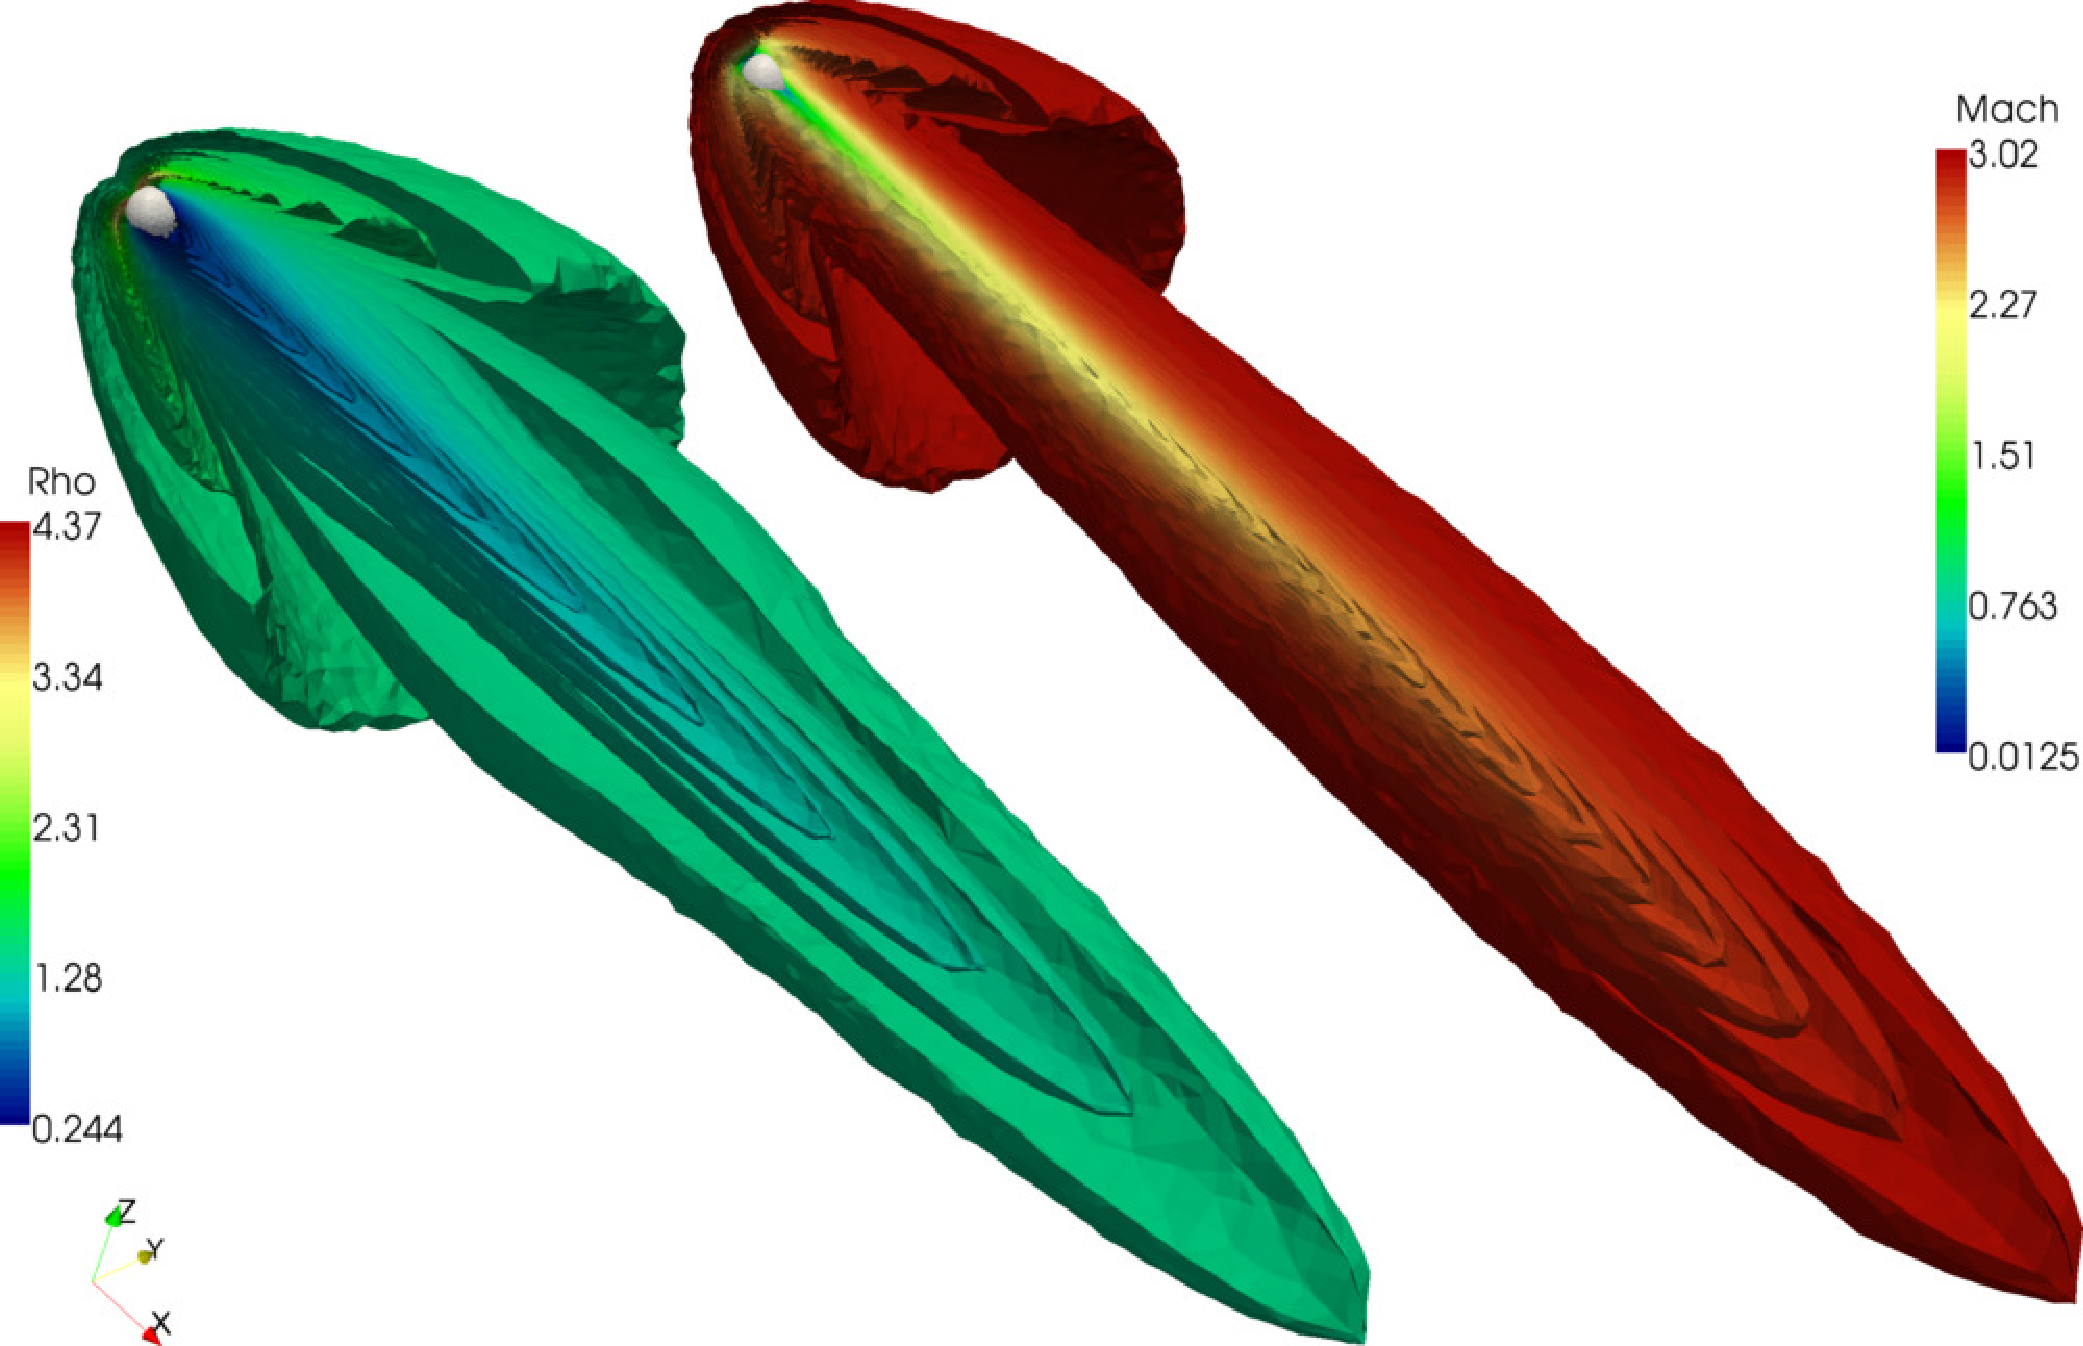
\includegraphics[width=10cm]{unfinished/hoffman-2/pdf/compressible3D.pdf}
}}
%\includegraphics[width=10cm]{media/unicorn_fsi_flag3D_01.pdf}
\caption{
Example application of adaptive computation of 3D compressible flow
around a sphere.  }
\label{fig:compr3D}
\end{figure}

\begin{figure}[!h]
\center{
\boxed{
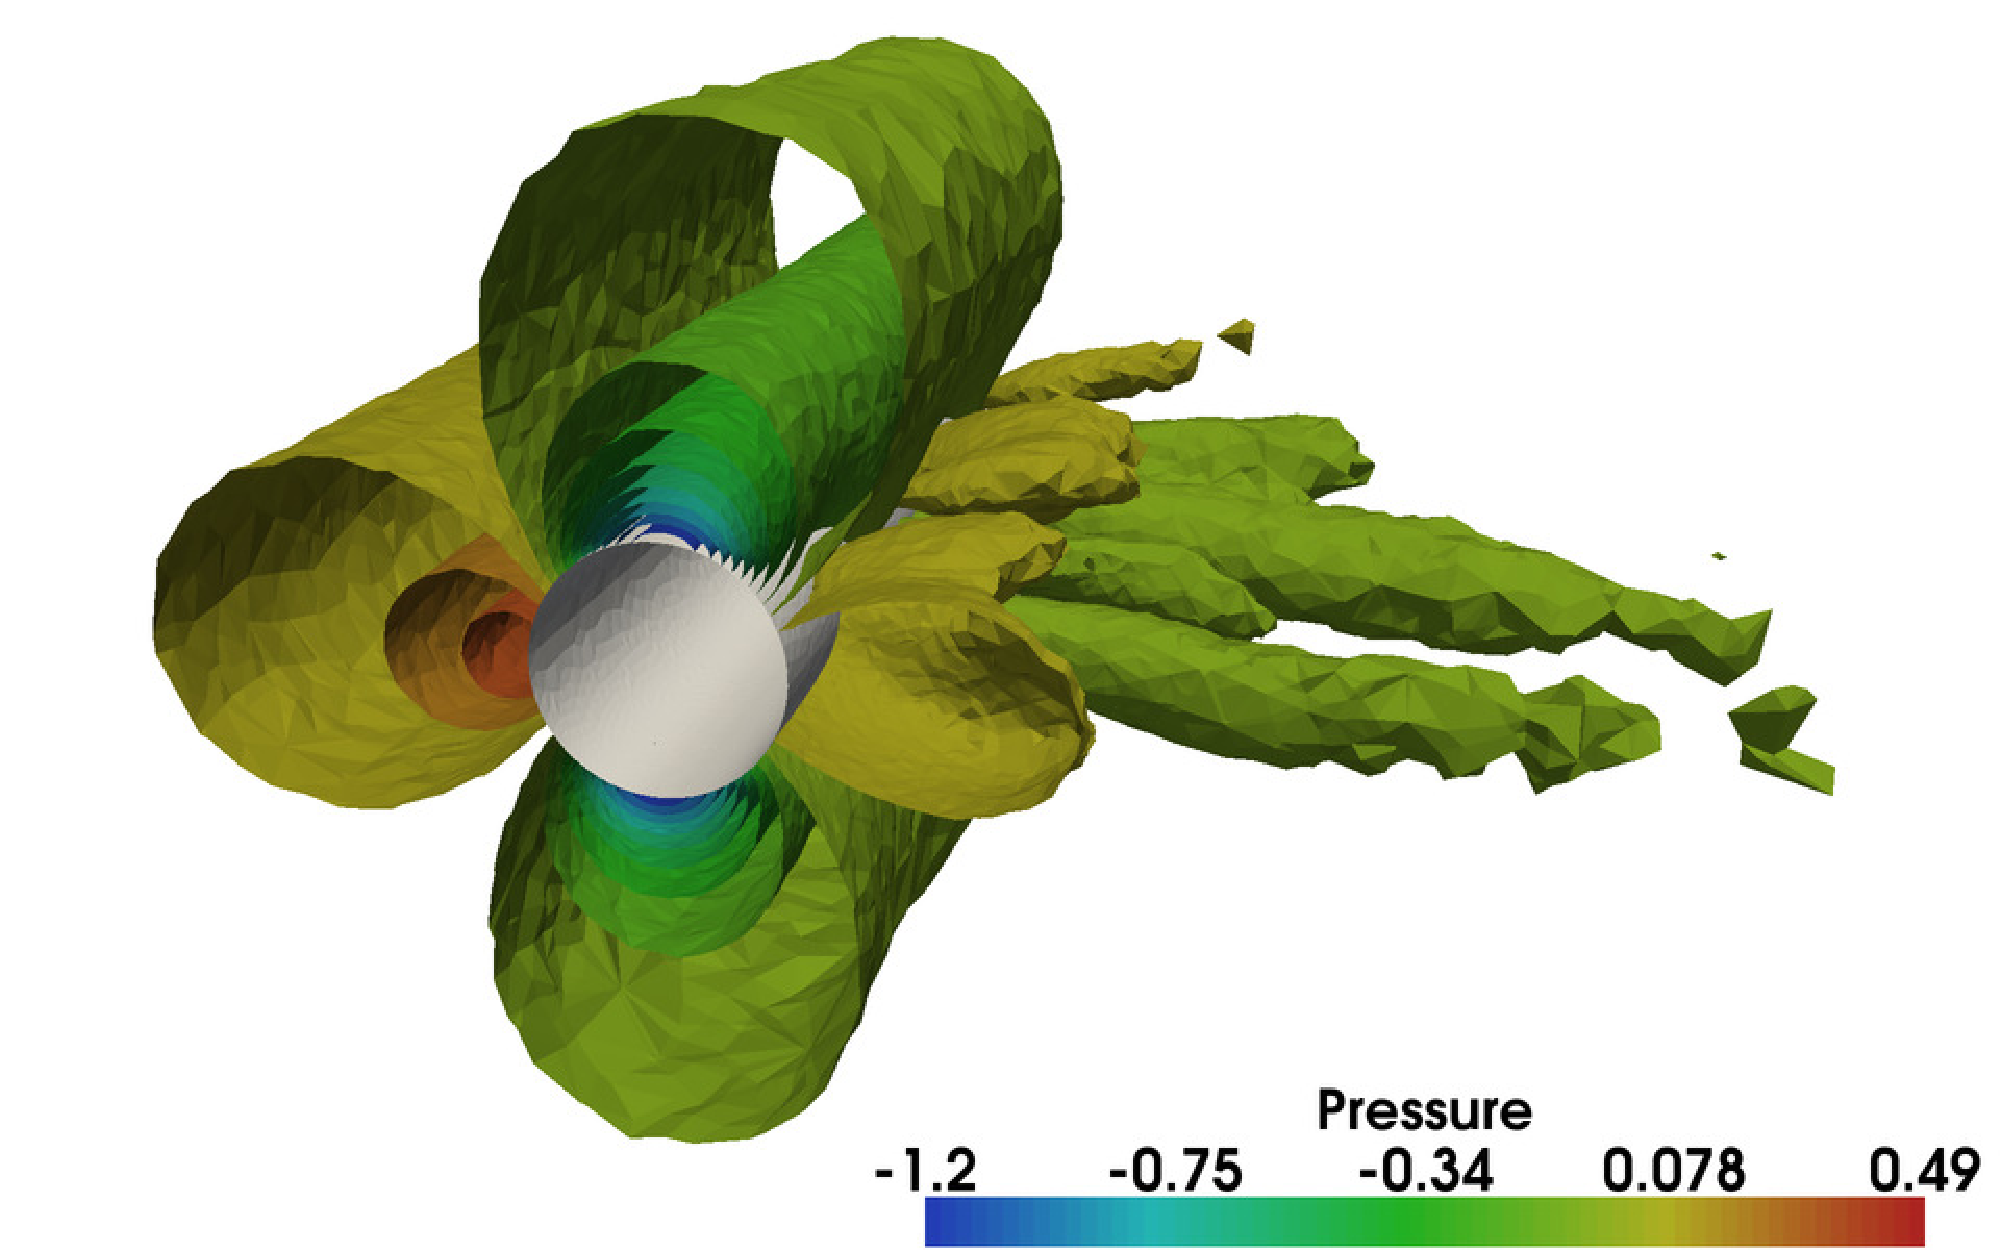
\includegraphics[width=10cm]{unfinished/hoffman-2/pdf/Hoffman_fig3d.pdf}
}}
%\includegraphics[width=10cm]{media/unicorn_fsi_flag3D_01.pdf}
\caption{
Example application of 3D turbulent incompressible flow around a
cylinder with parallel adaptive computation. }
\label{fig:parcyl3D}
\end{figure}


\label{chapter:implementation:unicorn}


%[Implementation: TimeDependentPDE, error estimation based on duality,
%mesh adaptivity/smoothing, friction BC, solver interface, efficient
%solution of discrete systems by fixed-point iteration, parallel
%solver/mesh refinement.]

%Write a short introduction to your chapter here. Explain the purpose
%of the chapter and include a brief outline. Remember to index
%important terms and use citations.~\cite{Ciarlet1978}

%\index{important term}

\section{Notation}

We occasionally use an indexed Einstein notation with the derivative of a
function $f$ with regard to the variable $x$ denoted as $D_x f$, and
the derivative with regard to component $x_i$ of component $f_j$
denoted as $D_{x_i} f_j = \nabla f_j$. Repeated indices denote a sum:
$D_{x_i} f_i = \sum_{i=1}^d D_{x_i} f_i = \nabla \cdot f$. Similarly
we can express derivatives with respect to any variable: $D_u u = 1$.
%------------------------------------------------------------------------------
\section{Unified continuum modeling}

% Intro (explain mesh motion)

We define, following classical continuum mechanics \cite{Gurtin1981}, a
unified continuum model in a fixed Euler coordinate system consisting
of:
\begin{itemize}
\item
conservation of mass
\item
conservation of momentum
\item
conservation of energy
\item
phase convection equation
\item
constitutive equations for stress as data
\end{itemize}
where the stress is the Cauchy (laboratory) stress and
the phase is an indicator function used to determine
which constitutive equation and material parameters to
use. Note that in this continuum description the
coordinate system is fixed (Euler), and a phase
function (indicator) is convected according to the
phase convection equation. However, since we typically
choose to also move the mesh (basis functions move in
time) one can think of this as an ALE method (see the
section ``Local ALE'': we introduce a local mesh
velocity, but we don't map back to a reference
configuration). Specifically we move the mesh with the
continuum velocity in the case of a solid phase to
eliminate diffusion of the phase interface.

We define two variants of this model: incompressible and compressible,
where a future aim is to construct a unified
incompressible/compressible model and solver. We focus the
presentation on the incompressible model, and therefore the discussion
of the energy $e$ is kept to a minimum (since it decouples and is not
considered).

We start with a model for conservation of mass, momentum and energy,
together with a convection equation for a phase function $\theta$ over
a space-time domain $Q = \Omega \times [0, T]$ with $\Omega$ an open
domain in $\mathbb{R}^3$ with boundary $\Gamma$:
\begin{equation}
  \addtolength{\fboxsep}{5pt}
  \boxed{
    \begin{split}\label{eq:TotalModel}
      D_t \rho + D_{x_j} (u_j \rho) &= 0
      \quad \text{(Mass conservation)}\\
      D_t m_i + D_{x_j} (u_j m_i) &= D_{x_j} \sigma_i
      \quad \text{(Momentum conservation)}\\
      D_t e + D_{x_j} (u_j e) &= D_{x_j} \sigma_i u_i
      \quad \text{(Energy conservation)}\\
      D_t \theta + D_{x_j} u_j \theta &= 0
      \quad \text{(Phase convection equation)}
    \end{split}
  }
\end{equation}
together with initial and boundary conditions, where $\rho$ is
density, $m_i$ is momentum, $u_i$ is velocity and $e$ is energy. We
can then pose constitutive relations between the constitutive (Cauchy)
stress component $\sigma$ and other variables such as the velocity
$u$. 

We define incompressibility in the usual way as:
\begin{align}
D_t \rho + u_j D_{x_j} \rho &= 0
\end{align}

which together with mass and momentum conservation gives:
\begin{align}
\rho(D_t u_i + u_j D_j u_i) &= D_{x_j} \sigma_{ij}\\
D_{x_j} u_j &= 0
\end{align}
where now the energy equation is decoupled and we omit it for simplicity.

We decompose the total stress into constitutive and forcing stresses:
\begin{align}
D_{x_j} \sigma_{ij} = D_{x_j} \sigma_{ij} + D_{x_j} \sigma^f_{ij} =
D_{x_j} \sigma_{ij} + f_i
\end{align}

Summarizing, we end up with the incompressible UC formulation:
\begin{equation}
  \addtolength{\fboxsep}{5pt}
  \boxed{
    \begin{split}\label{eq:TotalUC}
      \rho(D_t u_i + u_j D_{x_j} u_i) &= D_{x_j} \sigma_{ij} + f_i\\
      D_{x_j} u_j &= 0\\
      D_t \theta + D_{x_j} u_j \theta &= 0
    \end{split}
  }
\end{equation}
The UC modeling framework is simple and compact, close to the
formulation of the original conservation equations, without mappings
between coordinate systems. This allows simple manipulation and
processing for error estimation and implementation. It is also
general, we can choose the constitutive equations to model simple or
complex solids and fluids, possibly both in interaction, with
individual parameters. For examples how to use common constitutive
laws, see below.

\subsection{Automated computational modeling and software design}

One key design choice of UC modeling is to define the Cauchy stress
$\sigma$ as data, which means the conservation equations are fixed
regardless of the choice of constitutive equation. This gives a
generality in method and software design, where a modification of
constitutive equation impacts the formulation and implementation of the
constitutive equation, but not the formulation and implementation of the
conservation equations.

In Unicorn we choose an Euler coordinate system and moving mesh,
allowing a unified and canonical formulation of conservation
equations. This enables automated computational modeling (with
discretization and error control) for full fluid-structure (or
multi-phase) problems, rather than to one component at a time, with
unclear strategy how to combine them. We believe this is a unique
method/software system in this respect.

\section{Space-time general galerkin discretization}

Adaptive G2 methods (also referred to as Adaptive
DNS/LES) have been used in a number of turbulent flow
computations to a very low computational
cost \cite{Hoffman2005,HoffmanJohnson2006b,Hoffman2006,Hoffman2009,HoffmanJansson2009,VilelaJanssonEtAl2010},
where convergence is obtained in output quantities
such as drag, lift and pressure coefficients and
Strouhal numbers, using orders of magnitude fewer
numbers of mesh points than with LES methods based on
ad hoc refined computational meshes in the literature.

We begin by describing the standard FEM applied to the model to
establish basic notation, and proceed to describe streamline diffusion
stabilization and local ALE map over a mesh $T^h$ with mesh size $h$
together with adaptive error control based on duality.

\subsection{Standard galerkin}

We begin by formulating the standard cG(1)cG(1) FEM
\cite{ErikssonEstepHansboEtAl1996} with piecewise continuous linear solution in time
and space for \ref{eq:TotalModel} by defining the exact solution: $w =
[u, p, \theta]$, the discrete solution $W = [U, P, \Theta]$, the
test function $v = [v^u, v^p, v^\theta]$ and the residual $R(W) =
[R_u(W), R_p(W), R_\theta(W)]$:

\begin{align}
  R_u(W) &= \rho(D_t U_i + U_j D_{x_j} U_i) - D_{x_j} S_{ij} - f_i\\
  R_p(W) &= D_{x_j} U_j\\
  R_\theta(W) &= D_t \Theta + U_j D_{x_j} \Theta
\end{align}

where $R(w) = 0$ and $S$ denotes a discrete piecewise constant
stress. 

To determine the degrees of freedom $\xi$ we enforce the Galerkin
orthogonality $(R(W), v) = 0, \forall v \in V_h$ where $v$ are test
functions in the space of piecewise linear continuous functions in
space and piecewise constant discontinuous functions in time and
$(\cdot,\cdot)$ denotes the space-time $L_2$ inner product over Q. We
thus have the weak formulation:

\begin{align}
  (R^u(W), v^u) &= (\rho(D_t U_i + U_j D_j U_i) - f_i, v^u_i) + (S_{ij}, D_{x_j} v^u_i) - \int_{t_{n-1}}^{t_n}\int_\Gamma S_{ij} v^u_i n_j ds dt = 0\\
  (R^p(W), v^p) &= (D_{x_j} U_j, v^p) = 0\\
  (R^\theta(W), v^\theta) &= (D_t \Theta + u_j D_{x_j} \Theta, v^\theta) = 0
\end{align}

for all $v \in V_h$, where the boundary term on $\Gamma$ arising from
integration by parts vanishes if we assume a homogenous Neumann
boundary condition for the stress $S$.

This standard finite element formulation is unstable for
convection-dominated problems and due to choosing equal order for the
pressure and velocity. Thus we cannot use the standard finite element
formulation by itself but proceed to a streamline diffusion
stabilization formulation. We also describe a local ALE discretization
for handling the phase interface.

The cG(1)cG(1) formulation with trapezoid quadrature in time is
equivalent to Crank-Nicolson time-stepping with piecewise linear
elements in space. This has the advantage of being a very simple,
standard, and familiar discrete formulation. For the turbulent flow
mathematical model we use, the solutions are typically not smooth and
low order basis functions are thus sufficient.

\subsection{Local ALE}

If the phase function $\Theta$ has different values on
the same cell it would lead to an undesirable
diffusion of the phase interface. By introducing a
moving space-time finite element space and mesh,
oriented along the characteristics of the convection
of the phase
interface \cite{ErikssonEstepHansboEtAl1996} (see
space-time meshes in section ``The characterictic
Galerkin method'') we can define the phase interface
at cell facets, allowing the interface to stay
discontinuous.

We thus define a local ALE coordinate
map \cite{ErikssonEstepHansboEtAl1996} as part of the
discretization on each space-time slab, where it's
used to be able to introduce a mesh velocity. Note
that we still compute with global Euler coordinates
(we don't map back to a reference configuration), but
with a moving mesh.

The space-time FEM discretization gives a space-time
``slab'' $T_n \times I_n$ with $I_n = (t_{n-1}, t_n)$
and $T_n$ a triangulation of $\Omega$ for each time
step composed of the mesh cells over one time step.

To be able to define and compensate for an arbitrary
mesh velocity $\beta_h$ we define a local coordinate
map $\phi$ on each space-time slab:
\begin{equation}
\begin{split}\label{eq:ALEmap}
D_t \phi(t, \bar{x}) &= \beta_h(t, \bar{x})\\
(x, t) &= \phi(\bar{x}, t)\\
\end{split}
\end{equation}
Application of the chain rule gives the relation:
\begin{equation}
\begin{split}\label{eq:ALE2}
D_t U(x) + U(x) \cdot \nabla U(x) = D_t \bar{U}(\bar{x}) +
(\bar{U}(\bar{x}) - \beta_h)) \cdot \nabla \bar{U}(\bar{x})
\end{split}
\end{equation}
Space-time integration in a FEM gives (choosing simple
quadrature for clarity):
\begin{equation}
\begin{split}\label{eq:ALEFEM}
x_n &= F(\bar{x}) = \bar{x} + (t_n - t_{n - 1})\beta_h(\bar{x})\\
J &= D_{\bar{x}} F\\
\int_{K} u(t, x) dxdt &= \int_{\bar{K}} \bar{u}(t, \phi(t, \bar{x})) |det J| d\bar{x}dt
\end{split}
\end{equation}
We approximate $F = I$ in the integration and plan to
account for this in a posteriori error estimation,
since. $F$ is readily computable and $\|F - I\|$ is
likely small, given a reasonable size of $k$ and
$D_{\bar{x}} F$.

Choosing $\beta_h = U$ in the solid part of the mesh gives a trivial
solution of the phase convection equation, and we can remove it from
the system.

The resulting discrete UC
equations are:
\begin{equation}
\begin{split}\label{eq:ALE}
R_u(W) &= \rho(D_t U_i + (U_j - \beta^h_j) D_{x_j} U_i) - D_{x_j} S_{ij} - f_i\\
R_p(W) &= D_{x_j} U_j\\
R_\theta(W) &= D_t \Theta + (U_j - \beta^h_j) D_{x_j} \Theta
%D_t \Theta(x) +
%(U(x) - \beta_h(x)) \cdot \nabla \Theta(x) = 0
\end{split}
\end{equation}
with $\beta^h_j$ the mesh velocity.

We thus choose the mesh velocity $\beta_h$ to be the discrete material
velocity $U$ in the structure part of the mesh (vertices touching
structure cells) and in the rest of the mesh we use mesh smoothing to
determine $\beta_h$ to maximize the mesh quality according to a chosen
objective, alternatively use local mesh modification operations
(refinement, coarsening, swapping) on the mesh to maintain the quality
\cite{Comp`ereRemacleJanssonEtAl2009}.

\subsection{Streamline diffusion stabilization}

For the standard FEM formulation of the model we only have stability
of $U$ but not of spatial derivatives of $U$. This means the solution
can be oscillatory, causing inefficiency by introducing unnecessary
error. We instead choose a weighted standard Galerkin/streamline
diffusion method of the form $(R(W), v + \delta R(v)) = 0, \forall v
\in V_h$ (see \cite{ErikssonEstepHansboEtAl1996}) with $\delta > 0$ a stabilization
parameter. We here also make a simplification where we only introduce
necessary stabilization terms and drop terms not contributing to
stabilization. Although not fully consistent, the streamline diffusion
stabilization avoids unnecessary smearing of shear layers as the
stabilization is not based on large ($\approx h^{-\frac{1}{2}}$) cross flow
derivatives). For the UC model the stabilized method thus looks like:

\begin{align}
  (R^u(W), v^u) &= (\rho(D_t U_i + U_j D_j U_i) - f_i, v^u_i) + (S_{ij}, D_{x_j} v^u_i) + SD^u(W, v^u) = 0\\
  (R^p(W), v^p) &= (D_{x_j} U_j, v^p) + SD^p(W, v^p) = 0
\end{align}
for all $v \in V_h$, and:
\begin{align}
  SD^u(W, v^u) &= \delta_1 (U_j D_j U_i, U^u_j D_j v^u_i) +
  \delta_2 (D_{x_j} U_j, D_{x_j} v^u_j)\\
  SD^p(W, v^p) &= \delta_1 (D_{x_i} P, D_{x_i} v^p)
\end{align}

where we only include the dominating stabilization terms to reduce
complexity in the formulation.

\subsection{Unicorn software implementation}

We implement the G2 discretization of the UC (including adaptive error
control) in a general interface for time-dependent PDE where we give
the forms $a(U, v) = (D_U F_U, v)$ and $L(v) = (F_U, v)$ for
assembling the linear system given by Newton's method for a time step
for the incompressible UC with Newtonian fluid constitutive equation
in figure \ref{code:FFC_UC}. The language used is the
UFL \cite{KirbyLogg2006} form notation. In the adaptive error control,
we similarly represent residuals as forms in the form language, which
then allows us to compute error indicators using basic programming
constructs.

An overview of the interfaces and implementations of the Unicorn data
structures and algorithms are presented below.

\begin{figure}[!h]
\center{

\begin{python}

...

def ugradu(u, v):
    return [dot(u, grad(v[i])) for i in range(d)]

def epsilon(u):
    return 0.5 * (grad(u) + transp(grad(u)))

def S(u, P):
    return mult(P, Identity(d)) - mult(nu, grad(u))

def f(u, v):
    return -dot(ugradu(Uc, Uc), v) + \
        dot(S(Uc, P), grad(v)) + \
	-mult(d1, dot(ugradu(Um, u), ugradu(Um, v))) + \
	-mult(d2, dot(div(u), div(v))) + \
        dot(ff, v)

def dfdu(u, k, v):
    return -dot(ugradu(Um, u), v) + \
        -dot(mult(nu, grad(u)), grad(v)) + \
        -mult(d1, dot(ugradu(Um, u), ugradu(Um, v))) + \
        -mult(d2, dot(div(u), div(v)))

# cG(1)
def F(u, u0, k, v):
    uc = 0.5 * (u + u0)
    return (-dot(u, v) + dot(u0, v) + mult(k, f(u, v)))

def dFdu(u, u0, k, v):
    uc = 0.5 * u
    return (-dot(u, v) + mult(1.0 * k, dfdu(uc, k, v)))

a = (dFdu(U1, U0, k, v)) * dx
L = -F(UP, U0, k, v) * dx

\end{python}
}
\caption{
Source code for bilinear and linear forms for incompressible UC one
time step with a Newton-type method (approximation of Jacobian).  }
\label{code:FFC_UC}
\end{figure}

\section{Unicorn solver}

The Unicorn solver: {\tt UCSolver} ties together the technology in the
Unicorn library with other parts of FEniCS to expose an interface (see
listing \ref{code:UCSolver}) for simulating applications in continuum
mechanics. The main part of the solver implementation is the weak
forms for the G2 discretization of the UC model (see
listing \ref{code:FFC_UC}), together with forms for the stress and
residuals for the error estimation. Coefficients from the application
are connected to the form, and then time-stepping is carried out by
{\tt TimeDependentPDE}. Certain coefficients, such as the $\delta$
stabilization coefficients are also computed as part of the solver
(not as forms), where we aim to compute them as part of the forms. The
solver computes one iteration of the adaptive algorithm (primal solve,
dual solve and mesh refinement), where the adaptive loop is
implemented by iteratively running the solver for a sequence of
meshes.

The {\tt UCSolver} implementation is parallelized for distributed
memory architectures using MPI, and we can show strong scaling for
hundreds of cores on several platforms (see
Fig. \ref{fig:hoffman-2:sp}). The entire adaptive algorithm is
parallel (including Rivara mesh refinement and a priori predictive
load balancing) and Unicorn can efficiently simulate massively
parallel applications for turbulent incompressible
flow \cite{JanssonHoffmanJansson2010, Jansson2011}. Fluid-structure
interaction is not yet enabled in parallel but this is work in
progress.


\begin{figure}
\centering
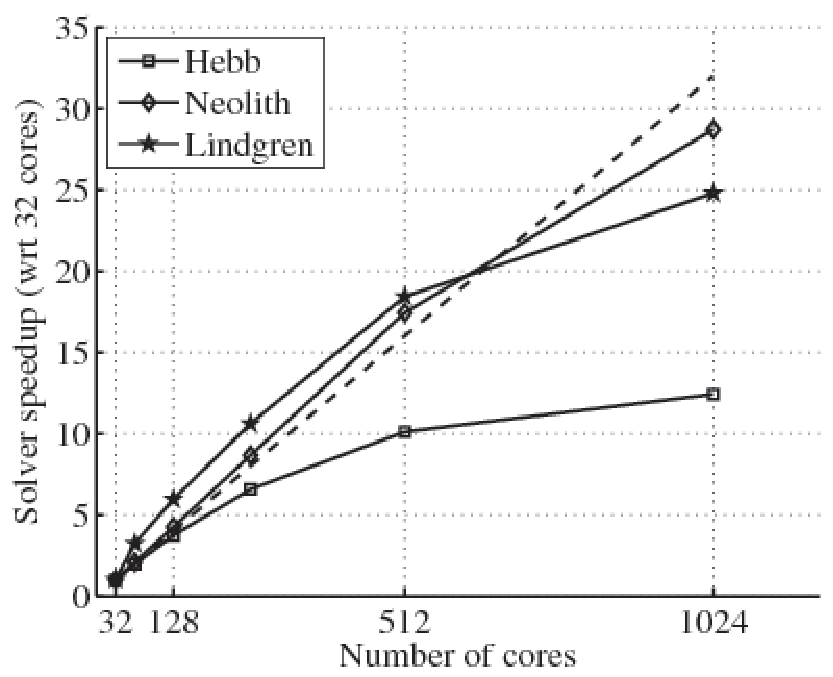
\includegraphics[height=5.5cm]{unfinished/hoffman-2/pdf/speedup_solve.pdf}
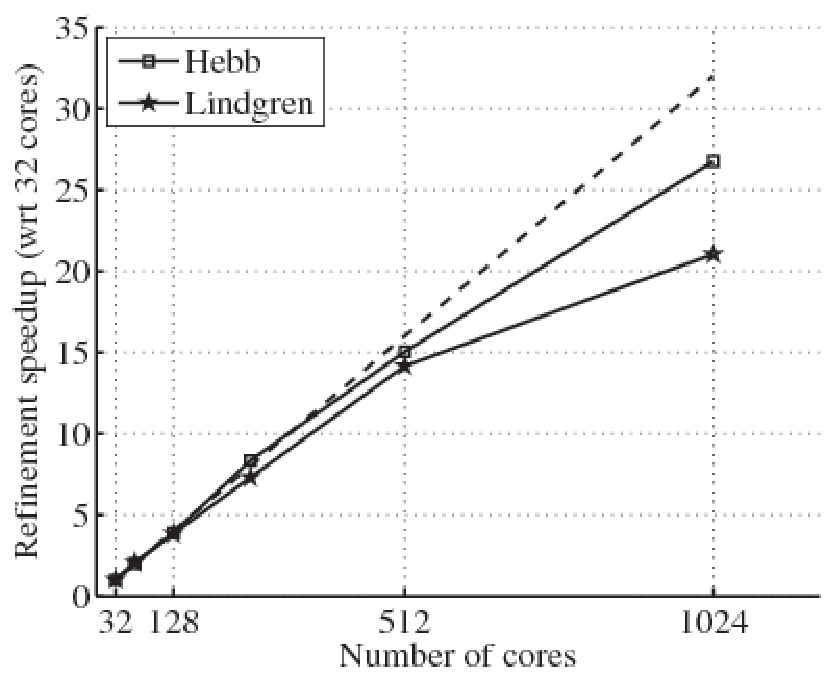
\includegraphics[height=5.5cm]{unfinished/hoffman-2/pdf/speedup_unrivara.pdf}
\caption{\label{fig:hoffman-2:sp} Strong scaling results for mesh refinement and entire solver on several different architectures, \textit{Lindgren} a Cray XT6m, \textit{Hebb} a BlueGene/L and \textit{Neolith} a regular Linux cluster with InfiniBand. The dashed line refers to ideal speedup}
\end{figure}


A compressible variant of the {\tt UCSolver} exists as the {\tt
  CNSSolver} for adaptive G2 for compressible Euler flow. The general
method and algorithm is very close to that of the {\tt UCSolver},
aside from the incompressibility. The long term goal is a unification
of the incompressible/compressible formulations as well. We refer to
\cite{Nazarov2009} for implementation details of the compressible {\tt
  CNSSolver}.

There also exists variants of the UC solver as part of the Unicorn
source code representing older formulations of the method, or pure
incompressible fluid formulations. These are used to verify that the
general {\tt UCSolver} does not introduce performance overhead or
implementation errors.

\begin{figure}[!p]
\begin{c++}
/// Unicorn implementation for the inc. UC model
class UCSolver :
  public TimeDependentPDE, public MeshAdaptInterface
{
public:
  /// Constructor: give boundary conditions,
  /// coefficients
  UCSolver(Function& U, Function& U0,
           Function** bisect, Mesh& mesh,
           Array <BoundaryCondition*>& bc_mom,
           Array <BoundaryCondition*>& bc_con,
           Function** f, real T, real nu,
           real mu, real rho_f, real rho_s,
           real u_bar, TimeDependent& t,
           PDEData* pdedata);

  /// Prescribe mesh size for MeshAdaptInterface
  virtual void updateSizeField();

  /// Allocate/deallocate PDE data for dynamic mesh
  /// adaptivity
  virtual void allocateAndComputeData();
  virtual void deallocateData();

  /// Compute mesh vertex coordinates and velocity
  void computeX();
  void computeW();

  /// Compute density, pressure, stress
  void computeRho();
  void computeP();
  void computeStress();

  /// Compute initial theta
  void computeTheta0();

  /// From TimeDependentPDE: time-stepping control
  void shift();
  bool update(real t, bool end);
  void preparestep();
  void prepareiteration();

  /// Assemble time step residual (L)/ right hand
  /// side of Newton
  void rhs(const Vector& x, Vector& dotx, real T);

  /// Compute initial value
  void u0(Vector& x); 

  /// Save solution/output quantities
  void save(Function& U, real t); 

  /// Compute least-squares stabilization parameters
  /// (delta)
  void computeStabilization(Mesh& mesh, Function& w,
                            real nu, real k, real t,
                            Vector& d1vector,
                            Vector& d2vector);

  /// Deform/move mesh
  void deform(Mesh& mesh, Function& W, Function& W0);

  /// Smooth/optimize quality of all or part of the
  /// mesh
  void smoothMesh(bool bAdaptive);
}
\end{c++}
\caption{
C++ class interface for the Unicorn solver: UCSolver.
}
\label{code:UCSolver}
\end{figure}



\begin{figure}[!p]
\begin{python}
(v1, v2, v3) = TestFunctions(TH) 
(rho, m, e) = TrialFunctions(TH)
(rho0, m0, e0) = Functions(TH)
...
# S prefix denotes stabilization:
# a1_a is Galerkin, S1_a is stabilization

# Bilinear form for density
a1_a = v1*rho*dx - k*0.5*dot(grad(v1),u)*rho*dx + \
 k*0.5*v1*rho*udotnormal*ds
S1_a = k*0.5*delta*dot(grad(v1),U)* \
 dot(U, grad(rho))*dx + \
 k*0.5*nu_rho*dot(grad(v1),grad(rho))*dx

# Linear form for the density
a1_L = v1*rho0*dx + k*0.5*dot(grad(v1),u)*rho0*dx - \
 k*0.5*v1*rho0*udotnormal*ds
S1_L = - k*0.5*delta*dot(grad(v1),U)* \
 dot(U, grad(rho0))*dx - \
 k*0.5*nu_rho*dot(grad(v1),grad(rho0))*dx

a2_a, S2_a, a2_L, S2_L = 0, 0, 0, 0

for i in range(0, d):
 # Bilinear form for momentum m_i
 a2_a += v2[i]*m[i]*dx - \
  k*0.5*dot(grad(v2[i]),u)*m[i]*dx + \
  k*0.5*v2[i]*m[i]*udotnormal*ds
 S2_a += k*0.5*delta*dot(grad(v2[i]),U)* \
  dot(U, grad(m[i]))*dx + \
  k*0.5*nu_m[i]*dot(grad(v2[i]),grad(m[i]))*dx
    
 # Linear form for the momentum
 a2_L += v2[i]*m0[i]*dx + \
  k*0.5*dot(grad(v2[i]),u)*m0[i]*dx + \
  k*v2[i].dx(i)*P*dx - \
  k*0.5*v2[i]*m0[i]*udotnormal*ds
 S2_L += -k*0.5*delta* \
  dot(grad(v2[i]),U)*dot(U, grad(m0[i]))*dx - \
  k*0.5*nu_m[i]*dot(grad(v2[i]),grad(m0[i]))*dx

# Bilinear form for energy
a3_a = v3*e*dx - k*0.5*dot(grad(v3),u)*e*dx + \
 k*0.5*v3*e*udotnormal*ds
S3_a = k*0.5*delta*dot(grad(v3),U)* \
 dot(U, grad(e))*dx + \
 k*0.5*nu_e*dot(grad(v3),grad(e))*dx

# Linear form for energy
a3_L = v3*e0*dx + k*0.5*dot(grad(v3),u)*e0*dx + \
 k*dot(grad(v3),u)*P*dx - k*0.5*v3*e0*udotnormal*ds
S3_L = - k*0.5*delta*dot(grad(v3),U)* \
 dot(U,grad(e0))*dx - \
 k*0.5*nu_e*dot(grad(v3),grad(e0))*dx

# Weak form of G2 for the Euler equations:
a = a1_a + S1_a + a2_a + S2_a + a3_a + S3_a
L = a1_L + S1_L + a2_L + S2_L + a3_L + S3_L
\end{python}
\caption{
Source code for bilinear and linear forms for G2 for compressible Euler one
time step with a Picard fixed-point iteration.  }
\label{code:form_compressible}
\end{figure}


\section{Unicorn library classes: data types and algorithms}

\subsection{Unicorn software design}

In software engineering there is a critical need to control software
complexity \cite{Brooks1995}. To achieve this, Unicorn follows two
basic design principles:

\begin{description}
\item[Prioritize simplicity of interfaces and implementation]
\ \\
We can rephrase this as the KISS principle: Keep It Simple and Stupid
\item[Avoid premature optimization]
\ \\
``Premature optimization is the root of all evil'' (Donald Knuth)]
\end{description}

Together, these two principles enforce generality and
understandability of interfaces and implementations. Unicorn re-uses
other existing implementations and chooses straightforward,
sufficiently efficient (optimize bottlenecks) standard algorithms for
solving problems. This leads to small, simple and maintainable
implementations. High performance is achieved by reducing the
computational load on the method level (adaptivity and fixed-point
iteration). 

\subsection{Unicorn classes/interfaces}

Unicorn consists of key concepts abstracted in the following
classes/interfaces:

\begin{description}
\item[{\tt TimeDependentPDE}: \ time-stepping]
\ \\
In each time-step a non-linear algebraic system is solved by
fixed-point iteration.
\item[{\tt ErrorEstimate}: \ adaptive error control]
\ \\
The adaptive algorithm is based on computing local {\em error
indicators} of the form $\epsilon_K = \|h R(U)\|_K \|D \phi\|_K$.

\item[{\tt SpaceTimeFunction}: \ space-time coefficient]
\ \\
Storage and evaluation of a space-time function/coefficient.
\item[{\tt SlipBC}: \ friction boundary condition]
\ \\
Efficient computation of turbulent flow in Unicorn is based on
modeling of turbulent boundary layers by a friction model, where the
normal condition: $u \cdot n = 0, x \in \Gamma$, is implemented as a
strong boundary condition in the algebraic system.
\item[{\tt ElasticSmoother}: \ elastic mesh smoothing/optimization]
\ \\
Optimization of cell quality according to an elastic analogy.
\item[{\tt MeshAdaptInterface}: \ mesh adaptation interface]
\ \\
Abstraction of the interface to the MAdLib package for mesh adaptation
using local mesh operations.
\end{description}

\subsection{\tt TimeDependentPDE}

We consider time-dependent equations of the type $f(u) = -D_t u + g(u)
= 0$ where $g$ can include differential operators in space, where
specifically the UC model is of this type. In weak form the equation
type looks like$(f(u), v) = (-D_t u + g(u), v) = 0$, possibly with
partial integration of terms

We want to define a class (datatype and algorithms) abstracting the
time-stepping of the G2 method, where we want to give the equation
(possibly in weak form) as input and generate the time-stepping
automatically. cG(1)cG(1) (Crank-Nicolson-type discretization in time)
gives the equation for the (possibly non-linear) algebraic system
$F(U)$ (in Python notation):


\begin{python}
# cG(1)
def F(u, u0, k, v):
    uc = 0.5 * (u + u0)
    return (-dot(u, v) + dot(u0, v) + mult(k, g(uc, v)))
\end{python}

By enforcing the above $\forall v \in V_h$ we generate the equation system.

We solve this system by Newton-type fixed-point iteration:

\begin{equation}
(F'(U_P) U_1, v) = (F'(U_P) - F(U_P), v)
\label{discrete_cg1}
\end{equation}

where $U_P$ denotes the value in the previous iterate and $F' = D_U F$
the Jacobian matrix or an approximation. Note that the choice of $F'$
only affects the convergence of the fixed-point iteration, and does
not introduce approximation error.

We define the bilinear form $a(U, v)$ and linear form $L(v)$
corresponding to the left and right hand sides respectively (in Python
notation):


{\small
\begin{python}
def dFdu(u, u0, k, v):
    uc = 0.5 * u
    return (-dot(u, v) + mult(k, dgdu(uc, k, v)))

a = (dFdu(U, U0, k, v)) * dx
L = (dFdu(UP, U0, k, v) - F(UP, U0, k, v)) * dx
\end{python}
}

Thus, in each time step we need to solve the system given in
eq. \ref{discrete_cg1} by fixed-point iteration by repeatedly
computing $a$ and $L$, solving a linear system and updating $U$.

We now encapsulate this in a C++ class interface in
fig. \ref{code:TimeDependentPDE} called {\tt TimeDependentPDE} where
$a$ and $L$, an end time $T$, a mesh (defining $V_h$) and
boundary conditions are given.



\begin{figure}[!h]
\begin{c++}
/// Represent and solve time dependent PDE.
class TimeDependentPDE
{
  /// Public interface
public:
  TimeDependentPDE(
   // Computational mesh
   Mesh& mesh,
   // Bilinear form for Jacobian approx.
   Form& a,
   // Linear form for time-step residual
   Form& L,
   // List of boundary conditions
   Array <BoundaryCondition*>& bcs,
   // End time
   real T);

  /// Solve PDE
  virtual uint solve();

protected:
  /// Compute initial value
  virtual void u0(Vector& u);
  /// Called before each time step
  virtual void preparestep();
  /// Called before each fixed-point iteration
  virtual void prepareiteration();
  /// Return the bilinear form a
  Form& a();
  /// Return the linear form L
  Form& L();
  /// Return the mesh
  Mesh& mesh();
};
\end{c++}
\caption{
C++ class interface for TimeDependentPDE.
}
\label{code:TimeDependentPDE}
\end{figure}


The skeleton of the time-stepping with fixed-point iteration is
implemented in listing \ref{code:time-stepping}.


\begin{figure}[!h]
{\small
\begin{c++}
void TimeDependentPDE::solve()
{
  // Time-stepping
  while(t < T)
  {
    U = U0;
    preparestep();
    step();
  }
}

void TimeDependentPDE::step()
{
  // Fixed-point iteration
  for(int iter = 0; iter < maxiter; iter++)
  {
    prepareiteration();
    step_residual = iter();

    if(step_residual < tol)
    {
      // Iteration converged
      break;
    }
  }
}

void TimeDependentPDE::iter()
{
  // Compute one fixed-point iteration
  assemble(J, a());
  assemble(b, L());
  for (uint i = 0; i < bc().size(); i++)
    bc()[i]->apply(J, b, a());
  solve(J, x, b);

  // Compute residual for the time-step/fixed-point
  // equation
  J.mult(x, residual);
  residual -= b;

  return residual.norm(linf);
}
\end{c++}
}
\label{code:time-stepping}
\caption{
Skeleton implementation in Unicorn of time-stepping with fixed-point
iteration.}
\end{figure}

To simplify the discussion, we consider Newton's method as a
linearization of the continuum model, where we then compute the
discretization of each successive iteration. A more general
formulation would be to compute Newton's method of the
discretization. For many cases this would be equivalent formulations,
since $D_U (F(U), v) = (D_U F(U), v)$, but for a stabilized method
these formulations may not be the same.

We use a block-diagonal quasi-Newton method, where we start by
formulating the full Newton method and then drop terms off the
diagonal blocks. We also use the constitutive law as an identity to
express $\sigma$ in terms of $U$, allowing larger time steps than
would be possibly otherwise by iterating between $\sigma$ and $U$. We
formulate Newton's method for the system $F(X) = (F_u(X), F_\sigma(X),
F_p(X))^\top = 0$, with $X = (U, \sigma, P)^\top$, where the three
components are decoupled.

See \cite{Jansson2009} for a dicussion about
the efficiency of the fixed-point iteration and its implementation.

\subsection{\tt ErrorEstimate}

The duality-based adaptive error control algorithm requires the
following primitives:

\begin{description}
\item[Residual computation]
We compute the mean-value in each cell of the continuous residual
$R(U) = f(U) = -D_t U + g(U)$, this is computed as the
$L_2$-projection into the space of piecewise constants $W_h$: $(R(U),
v) = (-D_t U + g(U), v), \forall v \in W_h$ (the mean value in each
cell) as a form representing the continuous residual.
\item[Dual solution]
We compute the solution of the dual problem using the same technology
as the primal problem. The dual problem is solved backward in time,
but with the time coordinate transform $s = T - t$ we can use the
standard {\tt TimeDependentPDE} interface and step the dual time $s$
forward.
\item[Space-time function storage/evaluation]
We compute error indicators while solving the dual problem as
space-time integrals over cells: $\epsilon_K = (R(U),
D_x \Phi)_{L_2(K \times T)}$, where we need to evaluate both the
primal solution $U$ and the dual solution $\Phi$. In addition, $U$ is
a coefficient in the dual equation. This requires storage and
evaluation of a space-time function, which is encapsulated in the {\tt
SpaceTimeFunction} class.
\item[Mesh adaptation]
After the computation of the error indicators we select the largest
$p\%$ of the indicators for refinement. The refinement is then
performed by recursive Rivara cell bisection or by general mesh
adaptation using Madlib \cite{Comp`ereRemacleJanssonEtAl2009}, which is
based on edge split, collapse and swap operations, and thus gives
the ability to coarsen a mesh, or more generally to control the mesh
size.
\end{description}

Using these primitives, we can construct an adaptive algorithm. The
adaptive algorithm is encapsulated in the C++ class interface in
fig. \ref{code:ErrorEstimate} which we call {\tt ErrorEstimate}.

\begin{figure}[!h]
{\small
\begin{c++}
/// Estimate error as local error indicators based
/// on duality
class ErrorEstimate
{
public:

  /// Constructor (give components of UC residual
  /// and dual solution)
  ErrorEstimate(Mesh& mesh,
		Form* Lres_1,
		Form* Lres_2,
		Form* Lres_3,
		Form* LDphi_1,
		Form* LDphi_2,
		Form* LDphi_3);

  // Compute error (norm estimate)
  void ComputeError(real& error);

  // Compute error indicator
  void ComputeErrorIndicator(real t, real k,
                             real T);

  // Compute largest indicators
  void ComputeLargestIndicators(
    std::vector<int>& cells,
    real percentage);
  
  // Refine based on indicators
  void AdaptiveRefinement(real percentage);
}
\end{c++}
}
\caption{
C++ class interface for {\tt ErrorEstimate}.
}
\label{code:ErrorEstimate}
\end{figure}

\subsection{\tt SpaceTimeFunction}

The error estimation algorithm requires, as part of solving the dual
problem, the evaluation of space-time coefficients (at time s in the
dual problem we need to evaluate the primal solution $U$ at time t = T
- s). This requires storage and evaluation of a space-time function,
which is encapsulated in the {\tt SpaceTimeFunction} class (see
listing \ref{code:SpaceTimeFunction}).

The space-time functionality is implemented as a list of space
functions at regular sample times, where evaluation is piecewise
linear interpolation in time of the values in the dofs.


\begin{figure}[!h]
{\small
\begin{c++}
/// Representation of space-time function (storage
/// and evaluation)
class SpaceTimeFunction
{
public:

  /// Create space-time function
  SpaceTimeFunction(Mesh& mesh, Function& Ut);

  /// Evaluate function at time t, giving result in
  /// Ut
  void eval(real t);

  // Add a space function at time t
  void addPoint(std::string Uname, real t);

  /// Return mesh associated with function
  Mesh& mesh();

  /// Return interpolant function
  Function& evaluant();
}
\end{c++}
}
\caption{
C++ class interface for {\tt SpaceTimeFunction}.
}
\label{code:SpaceTimeFunction}
\end{figure}



\subsection{\tt SlipBC}

For high Reynolds numbers problems such as car aerodynamics or
airplane flight, it's not possible to resolve the turbulent boundary
layer. One possibility is to model turbulent boundary layers by a
friction model:

\begin{align}
u \cdot n &= 0\\
\beta u \cdot \tau_k + n^\top \sigma \tau_k &= 0, k = 1, 2
\end{align}

We implement the normal component condition (slip) boundary condition
strongly. By ``strongly'' we here mean an implementation of the
boundary condition after assembling the left hand side matrix and the
right hand side vector in the algebraic system, whereas the tangential
components (friction) are implemented ``weakly'' by adding boundary
integrals in the variational formulation.  The row of the matrix and
load vector corresponding to a degree of freedom is found and replaced
by a new row according to the boundary condition.

The idea is as follows: Initially, the test function $v$ is expressed
in the Cartesian standard basis $(e_1, e_2, e_3)$.  Now, the test
function is mapped locally to normal-tangent coordinates with the
basis $(n, \tau_1, \tau_2)$, where $n = (n_1, n_2, n_3)$ is the
normal, and $\tau_1 = (\tau_{11}, \tau_{12}, \tau_{13})$, $\tau_2 =
(\tau_{21}, \tau_{22}, \tau_{23})$ are tangents to each node on the
boundary. This allows us to let the normal direction to be constrained
and the tangent directions be free:
\begin{equation}
     v = (v \cdot n)n + (v \cdot \tau_1) \tau_1 + (v \cdot \tau_2) \tau_2.
\end{equation}
For the matrix and vector this means that the rows corresponding to
the boundary need to be multiplied with $n,\tau_1,\tau_2$,
respectively, and then the normal component of the velocity should be
set to 0.

This concept is encapsulated in the class {\tt SlipBC} which is a
subclass of \\ {\tt dolfin::BoundaryCondition} for representing strong
boundary conditions. The implementation is based on multiplying
elements of the matrix with components of $n,\tau_1,\tau_2$.

For more details about the implementation of slip boundary conditions
we refer to \cite{Nazarov2009}.

\subsection{\tt ElasticSmoother}


\begin{figure}[!h]
{\small
\begin{python}
def tomatrix(q):
    return [ [q[d * i + j] for i in range(d)] for j in range(d) ]

Fmatrix = tomatrix(F)
Fm = tomatrix(F)
F0m = tomatrix(F0)
vm = tomatrix(v)

# icv is inverse cell volume

def f(U, F, v):
    return (-dot(mult(Fm, grad(U)), vm) - \
     dot(mult(transp(grad(U)), Fm), vm)))

a = (dot(dotF, v)) * dx
L = (mult(icv, dot(F0m, vm) + \
  mult(k, f(U, F, vm)))) * dx
\end{python}
}
\caption{Source code for forms representing one time step for the deformation gradient (F) evolution in the elastic smoother variant of the UC model. }
\label{code:FFC_ElasticSmoother}
\end{figure}


\begin{figure}[!h]
\begin{center}
\begin{tabular}{cc}
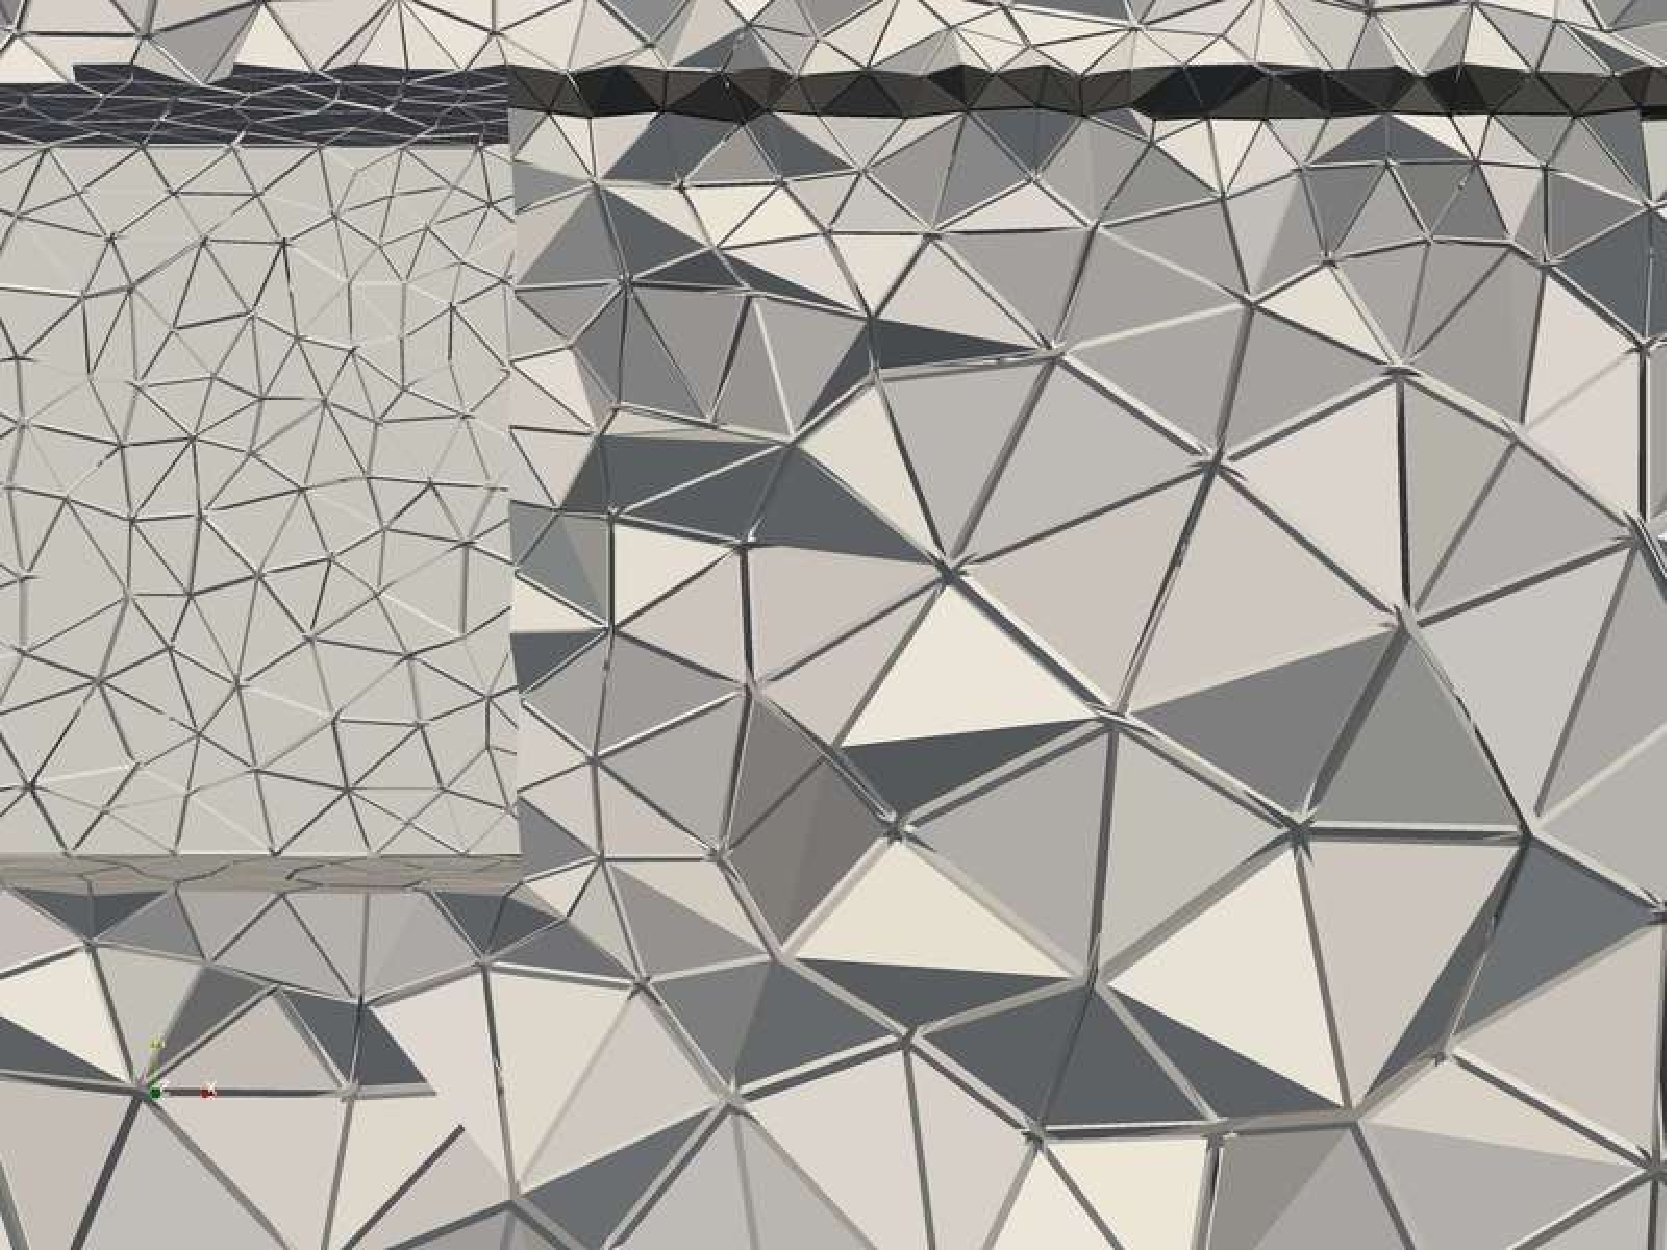
\includegraphics[height=0.24\linewidth]{unfinished/hoffman-2/pdf/force_smooth01.pdf} &
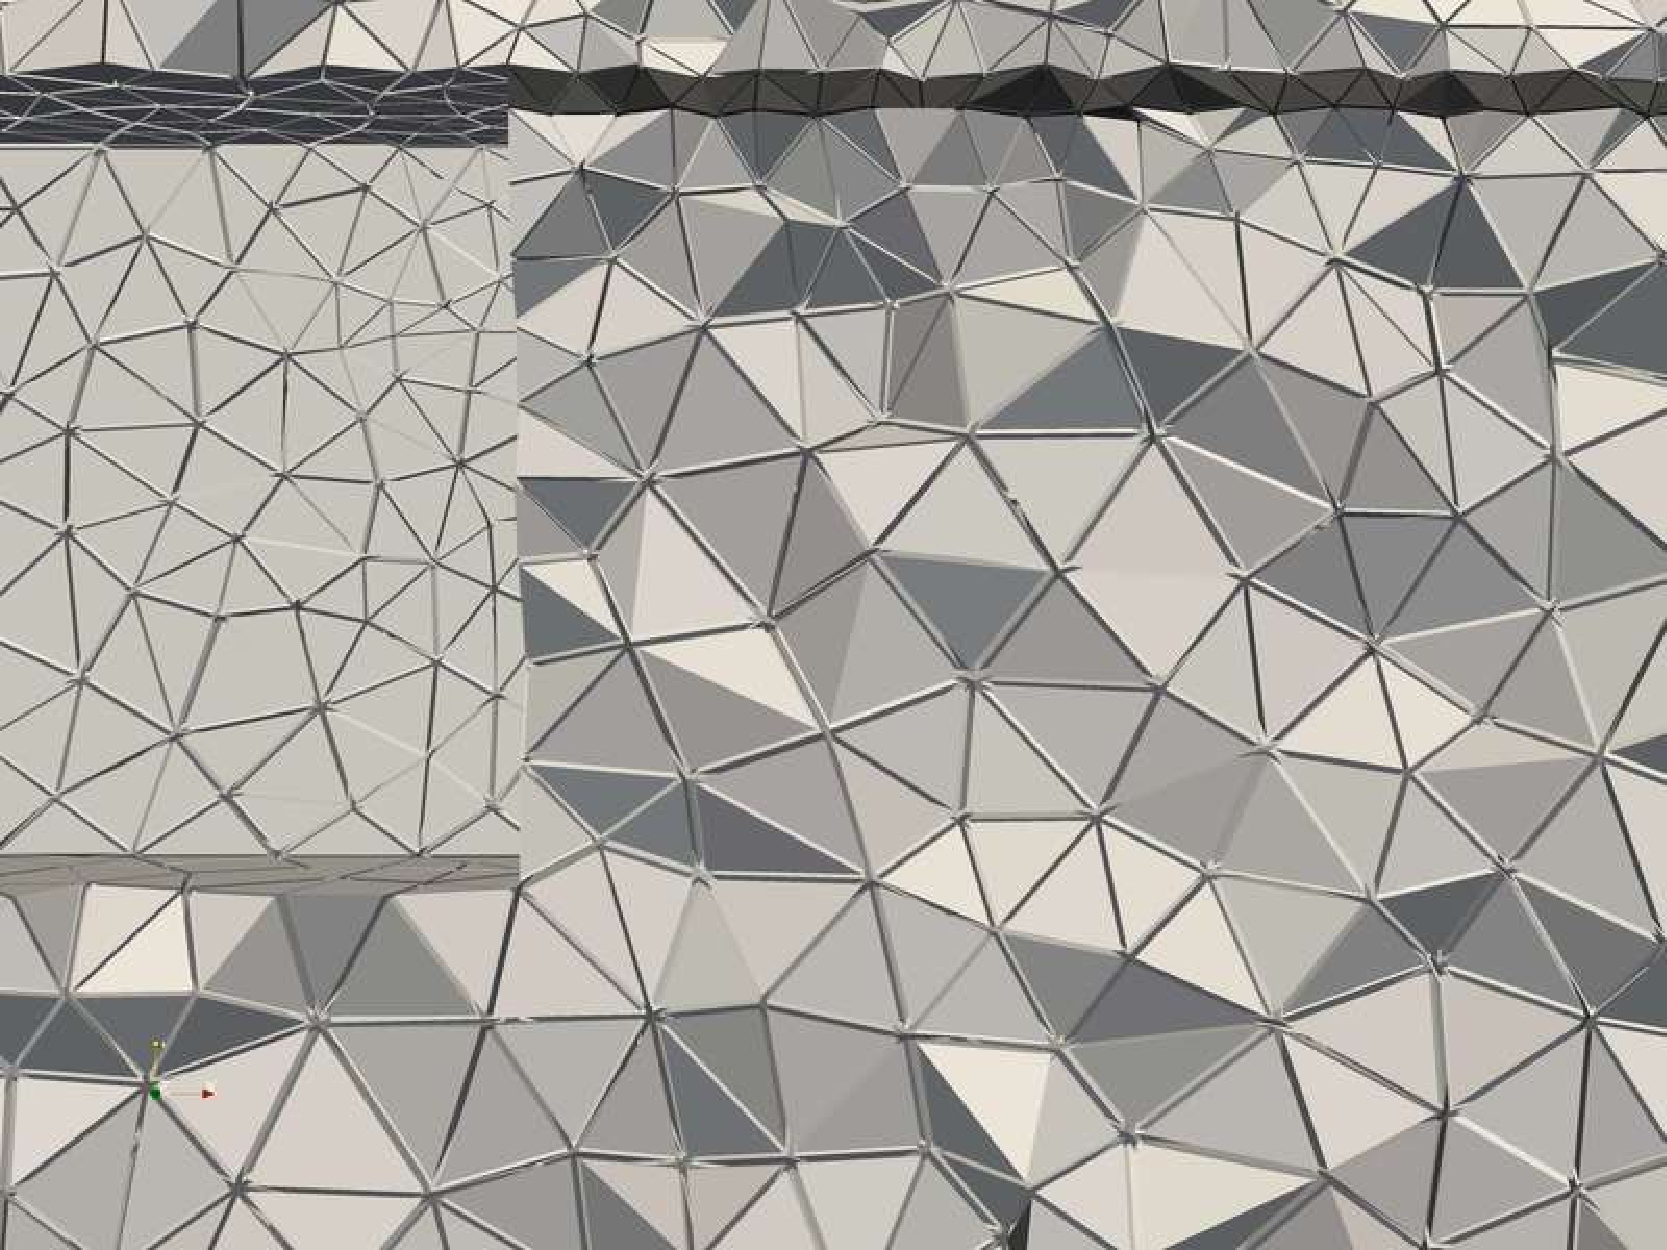
\includegraphics[height=0.24\linewidth]{unfinished/hoffman-2/pdf/force_hybrid01.pdf}\\
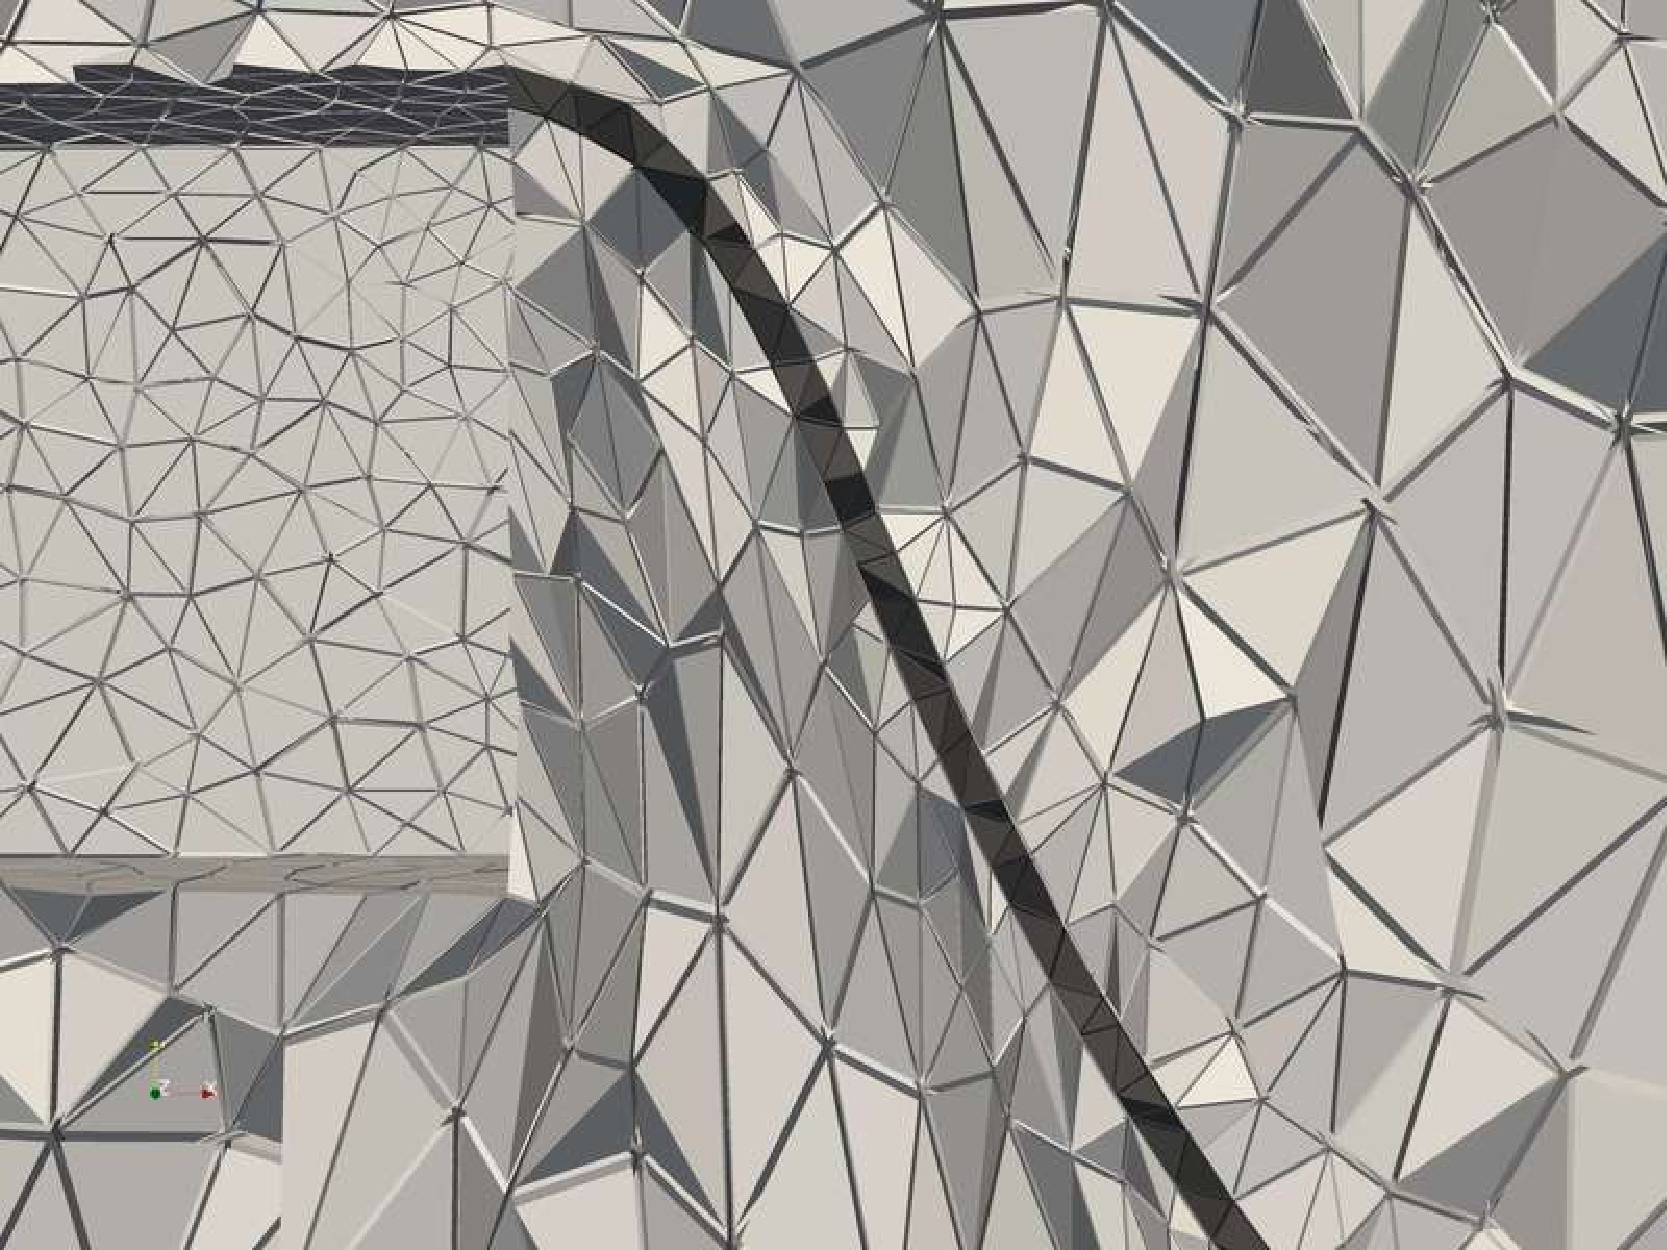
\includegraphics[height=0.24\linewidth]{unfinished/hoffman-2/pdf/force_smooth02.pdf} &
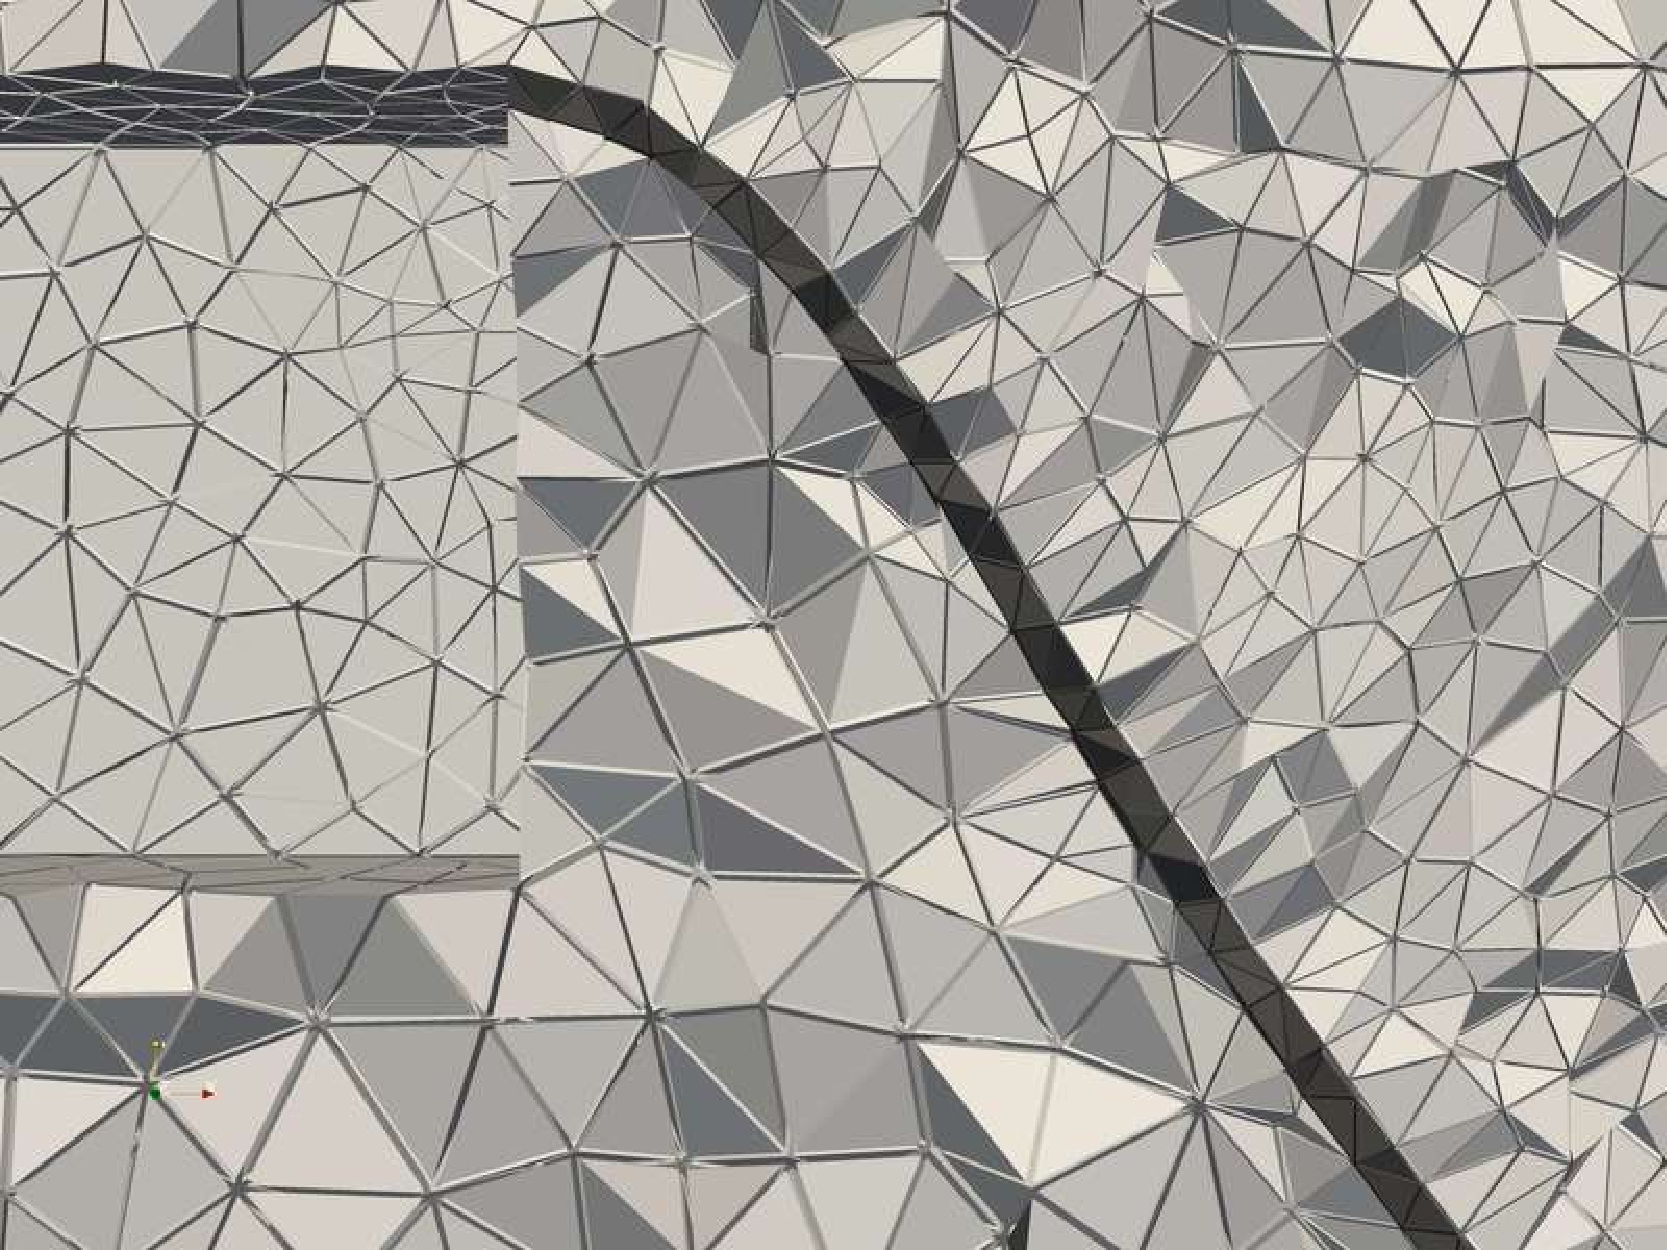
\includegraphics[height=0.24\linewidth]{unfinished/hoffman-2/pdf/force_hybrid02.pdf}\\
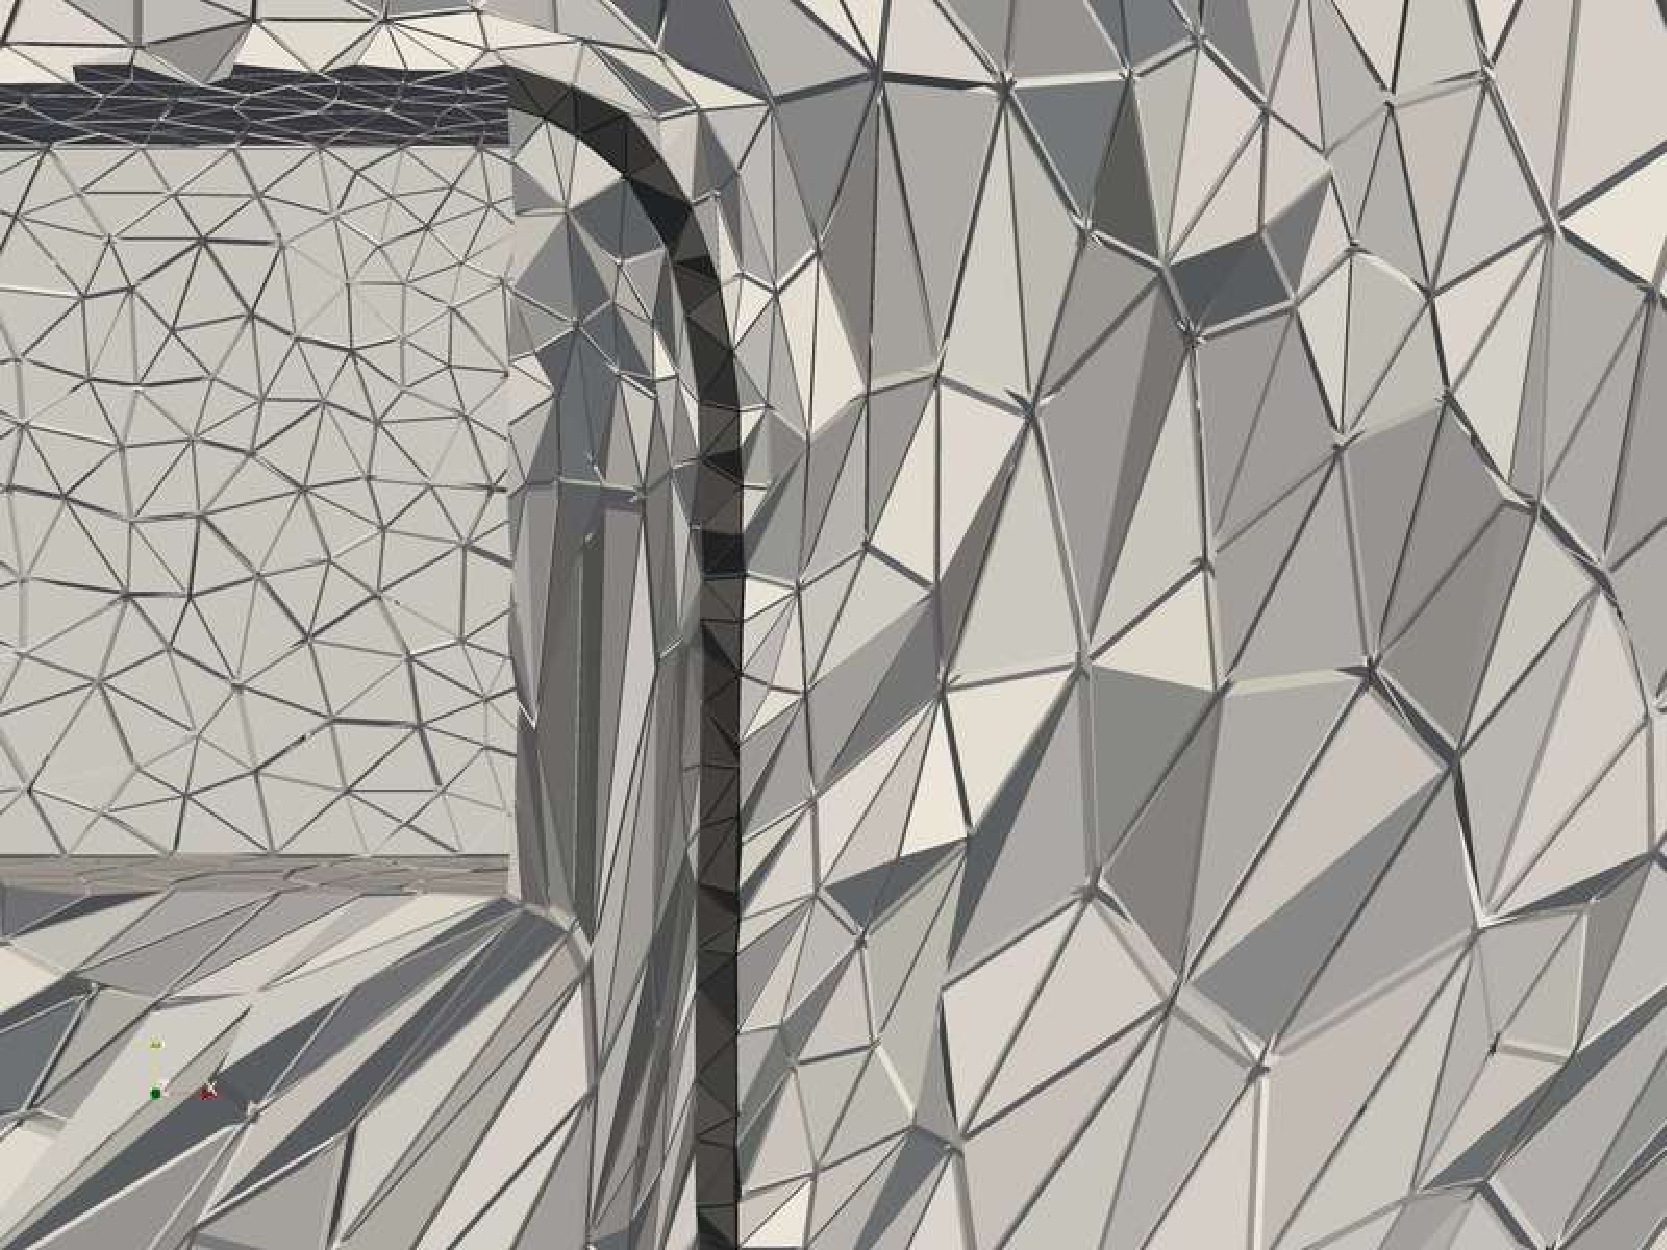
\includegraphics[height=0.24\linewidth]{unfinished/hoffman-2/pdf/force_smooth03.pdf} &
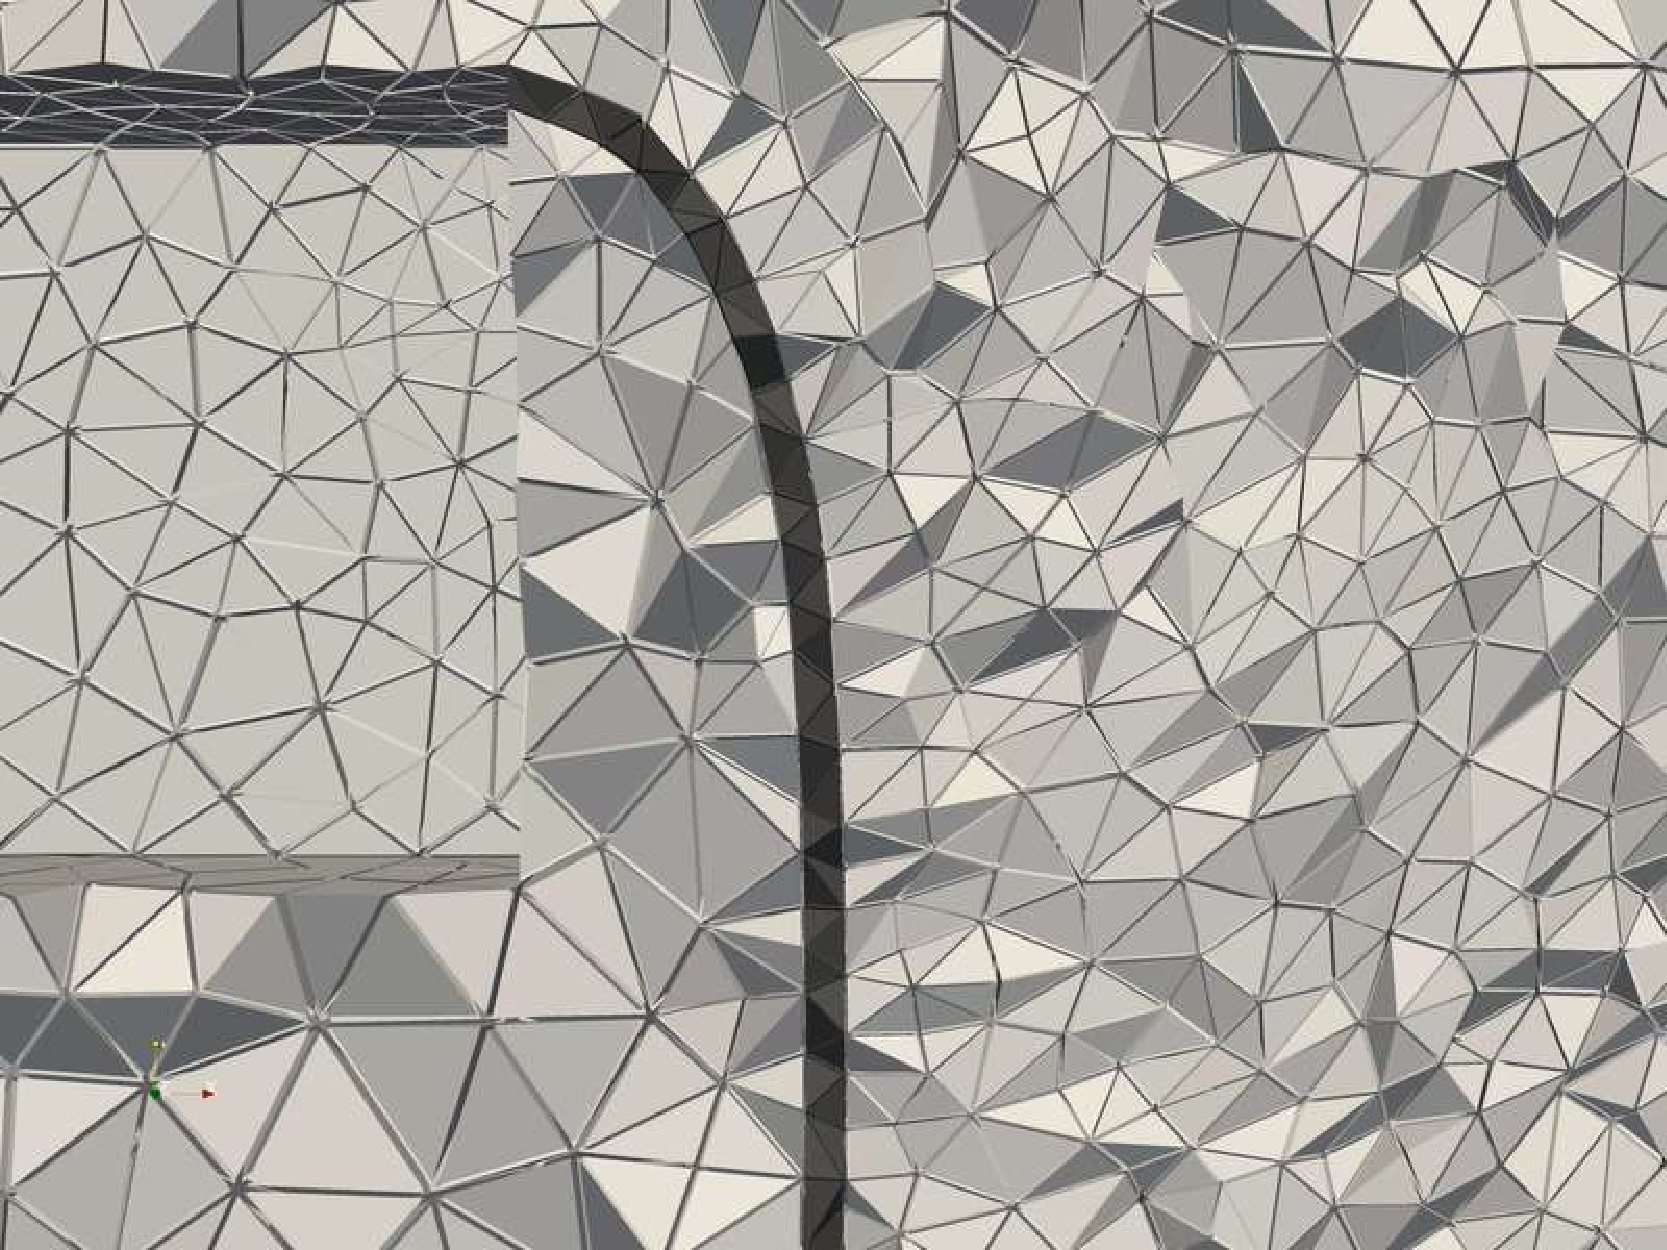
\includegraphics[height=0.24\linewidth]{unfinished/hoffman-2/pdf/force_hybrid03.pdf}\\
(a) & (b)
\end{tabular}
\end{center}
\caption{Robustness test with (a) elastic smoothing and (b) mesh adaptation. Note the badly shaped cells squeezed between the cube and flag.}
\label{fig:flag_robustness}
\end{figure}

\begin{figure}[!h]
{\scriptsize
\begin{c++}
/// Optimize cell quality according to elastic
/// variant of UC model
class ElasticSmoother
{
public:

  ElasticSmoother(Mesh& mesh);

  /// Smooth smoothed_cells giving mesh velocity W
  /// over time step k with h0 the prescribed cell
  /// size
  void smooth(MeshFunction<bool>& smoothed_cells,
              MeshFunction<bool>& masked_cells,
              MeshFunction<real>& h0,
              Function& W, real k);

  /// Extract submesh (for smoothing only marked cells)
  static void
  submesh(Mesh& mesh, Mesh& sub,
	  MeshFunction<bool>& smoothed_cells,
	  MeshFunction<int>& old2new_vertex,
	  MeshFunction<int>& old2new_cell);

}
\end{c++}
}
\caption{
C++ class interface for {\tt ElasticSmoother}.
}
\label{code:ElasticSmoother}
\end{figure}

To maintain a discontinuous phase interface in the UC with
fluid-structure data, we define the mesh velocity $\beta_h$ as the
discrete velocity $U$ in the solid phase (specifically on the
interface). The mesh velocity in the fluid can be chosen more
arbitrarily, but has to satisfy mesh quality and size criteria. We
construct a cell quality optimization/smoothing method based on a pure
elastic variant of the UC.

We define the following requirements for the mesh velocity $\beta_h$:

\begin{enumerate}
\item
$\beta_h = U$ in the solid phase part of the mesh.
\item
Bounded mesh quality $$Q = \frac{d \| F \|_F^2}{det(F)^{\frac{2}{d}}}$$  with $d$ the spatial dimension, in
the fluid part of the mesh. Preferably the mesh smoothing should
improve $Q$ if possible.
\item
Maintain mesh size $h(x)$ close to a desired $\hat{h}(x)$ given by a
posteriori error estimation in an adaptive algorithm.
%\item
%$\nabla \beta_h$ and $D_t \beta_h$ must be bounded.
\end{enumerate}

We formulate a simplistic variant of the UC model where we only
consider a solid, and we omit the incompressibility equation (see
listing \ref{code:FFC_ElasticSmoother}). We use a constitutive law
$\sigma = \mu(I - (FF^\top)^{-1})$ where we recall $F$ as the
deformation gradient. We use the update law: $D_t F^{-1} =
-F^{-1} \nabla u$ where we thus need an initial condition for $F$. We
set the initial condition $F_0 = \bar{F}$ where $\bar{F}$ is the
deformation gradient with regard to a scaled equilateral reference
cell, representing the optimal shape with quality $Q = 1$.

Solving the elastic model can thus be seen as optimizing for the
highest global quality $Q$ in the mesh. We also introduce a weight on
the Young's modulus $\mu$ for cells with low quality, penalizing high
average, but low local quality over mediocre global quality. We refer
to the source code for more details.

As an alternative to mesh smoothing we can consider using local mesh
modification operations (refinement, coarsening, swapping) on the mesh
to maintain the quality \cite{Comp`ereRemacleJanssonEtAl2009}
through {\tt MeshAdaptInterface}.

Unicorn provides the {\tt ElasticSmoother} class (see
listing \ref{code:ElasticSmoother}, which can be used to
smooth/optimize for quality in all or part of the mesh.

We perform a robustness test of the elastic smoothing and the mesh
adaptivity shown in \ref{fig:flag_robustness} where we use the same
geometry as the turbulent 3D flag problem, but define 0 inflow
velocity and instead add a gravity body force to the flag to create a
very large deformation with the flag pointing straight down. Both the
elastic smoothing and the mesh adaptvity compute solutions, but as
expected, the elastic mesh smoothing eventually cannot control the
cell quality (there does not exist a mesh motion which can handle
large rigid body rotations while bounding the cell quality).

\subsection{\tt MeshAdaptInterface}

A critical component in the adaptive algorithm as described above is
{\em Mesh adaptivity}, which we define as constructing a mesh
satisfying a given mesh size function $h(x)$.

We start by presenting the Rivara recursive bisection
algorithm \cite{Rivara1992} as a basic choice for mesh adaptivity
(currently the only available choice for parallel mesh adaptivity),
but which can only refine and not coarsen. Then the more general
MAdLib is presented, which enables the full mesh adaptation to the
prescribed $h(x)$ through local mesh operations: edge split, edge
collapse and edge swap.

\paragraph{Rivara recursive bisection}

The Rivara algorithm bisects (splits) the longest edge of a cell, thus
replacing the cell with two new cells, and uses recursive bisection to
eliminate non-conforming cells with hanging nodes. A non-conforming
cell $K_1$ has a neighbor (incident) cell $K_2$ that has a vertex on
an edge of cell $K_1$.

\begin{algorithm}
\caption{The Rivara recursive bisection algorithm}
\label{alg:rivara}
\begin{algorithmic}
\Procedure{bisect}{$K$}
\State Split longest edge $e$
\While{$K_i(e)$ is non-conforming}
\State BISECT($K_i$)
\EndWhile
\EndProcedure
\end{algorithmic}
\end{algorithm}

The same algorithm holds in both 2D/3D (triangles/tetrahedra). In 2D,
it can be shown \cite{Rivara1992} that the algorithm terminates in a
finite number of steps, and that the minimum angle of the refined mesh
is at least half the minimum angle of the starting mesh. In practice
the algorithm produces excellent quality refined meshes both in 2D and
3D.

\paragraph{Local mesh operations: Madlib}

 \begin{figure}[!h]
 \begin{center}
 \begin{tabular}{cc}
 \centering
 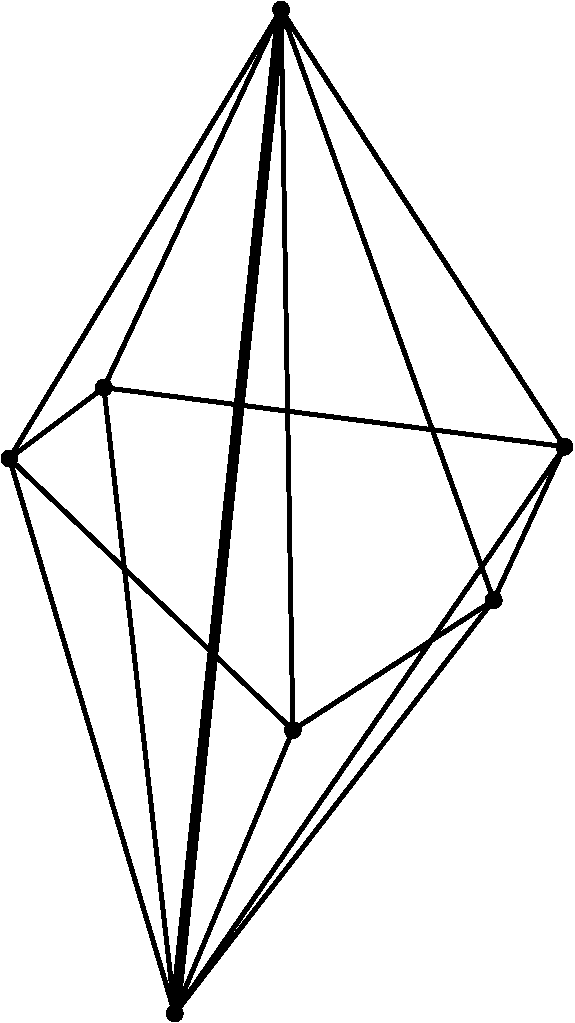
\includegraphics[height=3cm,width=6cm]{unfinished/hoffman-2/pdf/swap.pdf} &
 \hspace{0.3cm}
 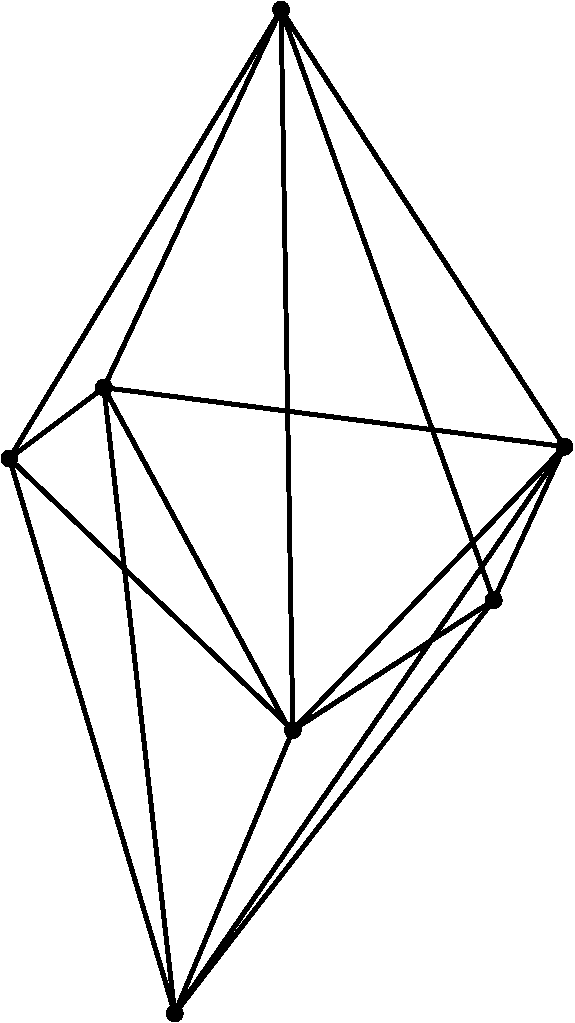
\includegraphics[height=3cm,width=6cm]{unfinished/hoffman-2/pdf/swap_config1.pdf}
 \end{tabular}
 \end{center}
 \caption{Edge swap operation: (a) initial cavity with swap edge highlighted (b) possible configuration after the swap.}
 \label{fig:op:eswap}
 \end{figure}

Madlib incorporates an algorithm and implementation of {\bf mesh
adaptation} where a small set of local mesh modification operators are
defined such as edge split, edge collapse and edge swap. A mesh
adaptation algorithm is defined which uses this set of local operators
in a control loop to satisfy a prescribed size field $h(x)$ and
quality tolerance. Edge swapping is the key operator for improving
quality of cells, for example around a vertex with a large number of
connected edges.

In the formulation of finite element methods it is typically assumed
that the cell size of a computational mesh can be freely modified to
satisfy a desired size field $h(x)$ or to allow mesh motion. In
state-of-the-art finite element software implementations this is
seldom the case, where typically only limited operations are allowed
\cite{BangerthHartmannKanschat2007, COMSOL2009}, (local mesh refinement),
or a separate often complex, closed and ad-hoc mesh generation
implementation is used to re-generate meshes.

The mesh adaptation algorithm in Madlib gives the freedom to adapt to
a specified size field using local mesh operations. The implementation
is published as free software/open source allowing other research to
build on the results and scientific repeatability of numerical
experiments.

Unicorn provides the {\tt MeshAdaptInterface} class (see
listing \ref{code:MeshAdaptInterface}, where one can subclass and
implement virtual functions to control the mesh adaptation.

We perform a robustness test of the elastic smoothing and the mesh
adaptivity shown in \ref{fig:flag_robustness}, see a more detailed
description in the elastic smoothing section.

\begin{figure}[!h]
\begin{c++}
/// Interface to MAdLib for mesh adaptation using
/// local operations Subclass and implement the
/// virtual functions
class MeshAdaptInterface
{
public:
  MeshAdaptInterface(Mesh *);
  
protected:
  /// Start mesh adaptation algorithm
  void adaptMesh();
  
  /// Give cell size field
  virtual void updateSizeField() = 0;
  
  /// Allocate and deallocate solver data
  virtual void deallocateData() = 0;
  virtual void allocateAndComputeData() = 0;
  
  /// Constrain entities not to be adapted
  void constrainExternalBoundaries();
  void constrainInternalBoundaries();
  
  /// Add functions to be automatically interpolated
  void addFunction(string name, Function** f);
  void clearFunctions();
};
\end{c++}
\caption{
C++ class interface for {\tt MeshAdaptInterface}.
}
\label{code:MeshAdaptInterface}
\end{figure}



\section{Solving continuum mechanics problems}

In this section we give use cases for modeling and solving continuum
mechanics problems using the Unicorn technology. We start with a use
case for solving a fluid-structure problem without adaptivity, where
we cover modeling of geometry and subdomains, coefficients, dynamic
allocation of PDE data for mesh adaptivity and specification of main
program (interface to running the solver). Next, we present a use case
for solving a turbulent pure fluid problem with adaptivity, where we
cover modeling of data for the dual problem, the adaptive loop, and
specifying slip/friction boundary conditions for modeling turbulent
boundary layers.


\subsection{Fluid-structure}

We here give a use case of solving a fluid-structure continuum
mechanics problem, where the user specifies data for modeling the
problem, and illustrates interfaces and expected outcomes. We divide
the use case into 4 parts:

\begin{description}
\item[Geometry and subdomains]
\ \\
The user specifies possible geometrical parameters and defines
subdomains. We note that for complex geometries the user may omit
geometry information and specify subdomain markers as data files.
\item[Coefficients]
\ \\
Known coefficients such as a force function and boundary conditions
are declared.
\item[PDE data]
\ \\
The user subclasses a PDEData class and specifies how the PDE data is
constructed and destroyed. This construction/destruction may happen
during the simulation if the mesh is adapted.
\item[main program]
\ \\
The user implements the main program and declares and passes data to
to the solver.
\end{description}

\subsection{Adaptivity}

We continue with a use case for adaptive solution of a pure fluid
turbulent flow problem: flow around a 3D cylinder. The implementation
of the problem is very similar to the fluid-structure case (just with
pure fluid data), but with 3 important additions:
\begin{description}
\item[Dual problem]
\ \\
To compute the error estimate required by the adaptive algorithm, we
must solve a dual problem generated by the primal problem and an
output quantity $\psi$. Since the dual problem is similar in form to
the primal problem, we implement both as variants of the same solver.

In this case we are interested in computing drag, which gives $\psi$
as a boundary condition for the dual problem:

\begin{c++}
CylinderBoundary cb;
SubSystem xcomp(0);
Function minus_one(mesh, -1.0);

DirichletBC dual_bc0(minus_one, mesh, cb, xcomp);

Array <BoundaryCondition*> dual_bc_mom;
dual_bc_mom.push_back(&dual_bc0);
\end{c++}


\item[Adaptive loop]
\ \\
We construct the program to compute one iteration of the adaptive
loop: solve primal problem, solve dual problem, compute error estimate
and check if tolerance is satisfied, compute adapted mesh. We can then
run the adaptive loop simply by a loop which runs the program (here in
Python which we also use to move data according to iteration number):


\begin{python}
offset = 0
N = 20

for i in range(offset, N):
    dirname = ``iter_%2.2d'' % i
    mkdir(dirname)

    system(``./unicorn-cylinder > log'')
    for file in glob(``./*.vtu''):
    move(file, dirname)
    for file in glob(``./*.pvd''):
    move(file, dirname)
\end{python}


\item[Slip boundary condition]
\ \\
For turbulent flow we model the boundary layer as a friction boundary
condition. We specify the normal component as a string slip boundary
condition used just as a regular Dirichlet boundary condition. The
{\tt xcomp} variable denotes an offset for the first velocity
component in a system (for compressible Euler the system is [density,
velocity, energy], and we would thus give component 2 as offset).

\begin{c++}
SlipBoundary sb;
SubSystem xcomp(0);

SlipBC slip_bc(mesh, sb, xcomp);

Array <BoundaryCondition*> primal_bc_mom;
primal_bc_mom.push_back(&slip_bc);
\end{c++}


\end{description}


\begin{figure}[!h]
\begin{c++}
#include <dolfin.h>
#include <unicorn/FSIPDE.h>

using namespace dolfin;
using namespace dolfin::unicorn;

real bmarg = 1.0e-3 + DOLFIN_EPS;

namespace Geo
{
  // Geometry details
  real box_L = 3.0;
  real box_H = 2.0;
  real box_W = 2.0;

  real xmin = 0.0; real xmax = box_L;
  real ymin = 0.0; real ymax = box_H;
  real zmin = 0.0; real zmax = box_W;
}

// Sub domain for inflow
class InflowBoundary3D : public SubDomain
{
public:
  bool inside(const real* p, bool on_boundary) const
  {
    return on_boundary && (p[0] < Geo::xmax - bmarg);
  }
};

// Sub domain for outflow
class OutflowBoundary3D : public SubDomain
{
public:
  bool inside(const real* p, bool on_boundary) const
  {
    return on_boundary && (p[0] > Geo::xmax - bmarg);
  }
};
\end{c++}
\caption{Part 1 of Unicorn solver FSI use case: geometry and subdomains.}
\end{figure}

\begin{figure}[!h]
\begin{c++}
// Force term
class ForceFunction : public Function
{
public:
  ForceFunction(Mesh& mesh, TimeDependent& td) : Function(mesh), td(td) {}
  void eval(real* values, const real* x) const
  {
    int d = cell().dim();

    for(int i = 0; i < d; i++)
    {
      values[i] = 0.0;
    }
  }

  TimeDependent& td;
};

// Boundary condition for momentum equation
class BC_Momentum_3D : public Function
{
public:
  BC_Momentum_3D(Mesh& mesh, TimeDependent& td) :
    Function(mesh), td(td) {}
  void eval(real* values, const real* x) const
  {
    int d = cell().dim();

    for(int i = 0; i < d; i++)
    {
      values[i] = 0.0;
    }
    if (x[0] < (Geo::xmin + bmarg))
      values[0] = 100.0;
  }

  TimeDependent& td;
};


// Initial condition for phase variable
class BisectionFunction : public Function
{
public:
  BisectionFunction(Mesh& mesh) : Function(mesh) {}
  void eval(real* values, const real* p) const
  {
    // NB: We specify the phase variable as
    // xml data so this function is not used

    bool condition = true;

    if (condition)
      values[0] = 0.0;
    else
      values[0] = 1.0;
  }
};
\end{c++}
\caption{Part 2 of Unicorn solver FSI use case: coefficients.}
\end{figure}

\begin{figure}[!h]
\begin{c++}
int main()
{
  Mesh mesh("flag.xml");

  real nu = 0.0;
  real nus = 0.5;
  real rhof = 1.0;
  real rhos = 1.0;

  real E = 1.0e6;

  real T = 0.2;

  dolfin::set("ODE number of samples", 500);

  Function U, U0;

  real u_bar = 100.0;

  FlagData pdedata;

  ICNSPDE pde(U, U0, &(pdedata.bisect), mesh,
	      pdedata.bc_mom, pdedata.bc_con,
	      &(pdedata.f), T, nu, E, nus, rhof, rhos,
	      u_bar, pdedata.td, &pdedata);

  // Compute solution
  pde.solve(U, U0);

  return 0;
}
\end{c++}
\caption{Part 4 of FSI use case: main program, passing data to solver.}
\end{figure}

\subsection{Unicorn-HPC installation and basic test}

Unicorn-HPC is the high-performance computing branch of Unicorn,
showing strong linear scaling on massively parallel hardware as
described above.

To verify the correct installation and functionality of Unicorn-HPC,
follow the steps in the README file in the Unicorn-HPC distribution,
under ``Testing''. The test represents the turbulent flow past a cube
simulation described in chapter \ref{chap:hoffman-1}.

\section{Acknowledgement}

We acknowledge contributions to Unicorn, both software development as
well as ideas and scientific support from: Mattias Aechtner, Peter
Brune, Zilan Ciftci, G\"aetan Compere, Niyazi Cem Degirmenci, Claes
Johnson, Ashraful Kadir, Jeannette Sp\"uhler, Michael St\"ockli and
Rodrigo Vilela de Abreu.



%\fenicsinput{mardal-2}
%
%\part{Applications}
%
%%%%\fenicsinput{terrel}
%\fenicsinput{kvs-1}
%\fenicsinput{mortensen}
%%\fenicschapter{Turbulent Flow and Fluid-Structure Interaction}
              {Turbulent Flow and Fluid-Structure Interaction}
              {Johan Hoffman, Johan Jansson, Niclas Jansson, Claes Johnson and Rodrigo Vilela De Abreu}
              {hoffman-1}

The FEniCS project aims towards the goals of
generality, efficiency, and simplicity, concerning
mathematical methodology, implementation, and
application, and the Unicorn project is an
implementation aimed at FSI and high Re turbulent flow
guided by these principles. Unicorn is based on the
DOLFIN/FFC/FIAT suite and the linear algebra package
PETSc, and we here present some key elements of
Unicorn, and a set of computational results from
applications. The details of the Unicorn
implementation is described in
Chapter~\ref{chap:hoffman-2}.

\section{Background}

For many problems involving a fluid and a structure,
decoupling the computation of the two is not feasible
for accurate modeling of the phenomenon at hand,
instead the full fluid-structure interaction (FSI)
problem has to be solved together as a coupled
problem. This includes a multitude of important
problems in biology, medicine and industry, such as
the simulation of insect or bird flight, the human
cardiovascular and respiratory systems, the human
speech organ, the paper making process, acoustic noise
generation in exhaust systems, airplane wing flutter,
wind induced vibrations in bridges and wave loads on
offshore structures. Common for many of these problems
is that for various reasons they are very hard or
impossible to investigate experimentally, and thus
reliable computational simulation would open up for
detailed study and new insights, as well as for new
important design tools for construction.

Computational methods for FSI is a very active
research field today. In particular, major open
challenges of computational FSI include: (i)
robustness of the fluid-structure coupling, (ii) for
high Reynolds numbers (Re) the computation of
turbulent fluid flow, and (iii) efficiency and
reliability of the computations in the form of
adaptive methods and quantitative error estimation.

\section{Simulation of high Re turbulent flow}

The focus of Unicorn is high Re turbulent fluid flow, also including fluid-structure interaction. Direct numerical simulation (DNS) of turbulent flow is limited to moderate Re and simple geometry, due to the high computational cost of resolving all turbulent scales in the flow. The standard e.g. in the automotive industry is simulation based on Reynolds averaged Navier-Stokes equations (RANS), where time averages (or statistical averages) are computed to an affordable cost, with the drawback of introducing turbulence models based on parameters that have to be tuned for particular applications.

An alternative to DNS and RANS is Large eddy simulation (LES) \cite{Sagaut2005}, where a filter is applied to the Navier-Stokes equations to derive a new set of equations with a smallest scale given by the filter width, and where the effect of the filter is the introduction of so called subgrid stresses which need to be modeled in a subgrid model. A subgrid model can be motivated by physics theory or experiments, and the main effect of the subgrid model is to dissipate kinetic energy, for example in the form of turbulent viscosity.

Typically the numerical method used to approximate the LES equations also introduces dissipation, and thus there are two sources of kinetic energy dissipation; the subgrid model and the numerical method. One class of methods, Implicit LES (ILES), relies completely on the numerical method to act as subgrid model, without any additional explicit subgrid model \cite{Sagaut2005}. Turbulence simulation in Unicorn is based on ILES in the form a stabilized finite element method, referred to as a General Galerkin (G2) simulation \cite{HoffmanJohnson2007}, where a least squares stabilization based on the residual of the Navier-Stokes equations acts a an ILES subgrid model.

More specific, in the current G2/ILES implementation of Unicorn continuous piecewise linear approximation is used in space and time, together with a least squares stabilization based on the residual \cite{HoffmanJohnson2007}.

\section{Turbulent boundary layers}
\label{section:blayer}

The choice of boundary conditions at a solid wall is critical for accurate LES modeling of fluid flow, in particular to capture flow separation phenomena. In Unicorn, laminar boundary layers are fully resolved by the computational method by applying no slip (zero velocity) boundary conditions at the wall. On the other hand, computational resolution of turbulent boundary layers is only possible at limited Reynolds numbers and for simple geometries.

The standard way to model the effect of turbulent boundary layers is to divide the computational domain into: (i) an interior part $\Omega$, and (ii) a boundary layer region. In the boundary layer a simplified model of the flow is used to provide boundary conditions to the LES equations to be solved in the interior part $\Omega$. Boundary conditions are typically in the form of a wall shear stress, and the coupling between (i) and (ii) may be one-way from (ii) to (i), or more closely coupled. Wall shear stress models are developed based on experimental data, theory, or computation by a simplified model (e.g. a RANS model). For an overview of boundary layer modeling, see e.g. \cite{SagautDeckTerracol2006,PiomelliBalaras2002}.

The wall shear stress model in Unicorn takes a similar form as the simple Shumann model \cite{Schumann1975}, with the tangential velocity proportional to the local wall shear stress through a skin friction parameter (or function) $\beta$. That is, the following boundary conditions are used for the velocity $u$ and stress $\sigma$:
\begin{eqnarray}
&&u\cdot n=0, \label{slfra} \\
&&\beta u\cdot \tau _k + n^T\sigma \tau _k=0,\quad k=1,2, \label{slfrb}
\end{eqnarray}
for  $(x,t)\in \Gamma_{solid}\times [0,T]$, with $n=n(x)$ an outward unit normal vector, and $\tau_k=\tau_k(x)$ orthogonal unit tangent vectors of $\Gamma_{solid}$. Matrix notation is used, with all vectors $v$ being column vectors and the corresponding row vector is denoted $v^T$. The non-penetration boundary condition is applied strongly, whereas a weak implementation is used for the wall shear stress boundary condition.

\section{Adaptivity and a posteriori error estimation}

A posteriori error estimation involves only computable quantities, which opens for adaptive methods with quantitative error control. The basic idea of adaptive algorithms is to optimize the computational method with respect to the goal (output of interest) of the computation. Typical parameters of an adaptive finite element method include the local mesh size (h-adaptivity), local degree of the finite element approximation (p-adaptivity), local shape of the cells (r-adaptivity), or combinations thereof. Other possible parameters may be the time step size and the stabilization parameters.

In Unicorn, an approach to a posteriori error estimation is used where the error in a chosen output quantity can be estimated in terms of the solution of an associated linearized dual problem. The basic framework is described e.g. in the survey articles \cite{ErikssonEstepEtAl1995,BeckerRannacher2001,GilesSuli2002}.

Using standard techniques of a posteriori error analysis, an a posteriori error estimate for G2 can be derived in the following form:
\begin{equation}
\vert M(u) - M(U) \vert \leq \sum_K {\cal E}_K
\end{equation}
with $M(u)$ the target output to compute and $M(U)$ the approximation, with $U$ a G2 solution, and ${\cal E}_K$ a local error indicator for cell $K$.
The error indicator ${\cal E}_K$ is constructed from the residual, measuring local errors,
weighted by the solution to a dual (adjoint) problem measuring the effect of local errors
on the output $M(\cdot)$. The implementation of the dual problem in Unicorn is based on the cG(1)cG(1) method described in \cite{HoffmanJohnson2007}. The computational mesh is then modified according to $ {\cal E}_K$, by mesh refinement, coarsening or smoothing.

Adaptive G2 methods (also referred to as Adaptive DNS/LES) have been used in a number of turbulent flow computations to a very low computational cost \cite{Hoffman2005,HoffmanJohnson2006b,Hoffman2006,Hoffman2009,HoffmanJansson2009,VilelaJanssonEtAl2010}, where convergence is obtained in output quantities such as drag, lift and pressure coefficients and Strouhal numbers, using orders of magnitude fewer numbers of mesh points than with LES methods based on ad hoc refined computational meshes in the literature.

\section{Robust fluid-structure coupling}

In a computational method based on so called weakly coupled FSI, separate solvers can be used for the fluid and the structure, with the benefit of being able to reuse existing dedicated fluid and structure solvers. To couple the fluid and the structure, boundary data such as displacements and stresses is exchanged over the fluid-structure interface, either as part of a fixed-point iteration or in a fully explicit fashion. To make the coupling more robust the equations for the fluid and the structure can be placed in the same algebraic system together with all coupling conditions, corresponding to a so called strong FSI coupling.

Another approach is to formulate the fluid and the structure as one single continuum model, which is then said to be a monolithic FSI method. In Unicorn a monolithic method is used referred to as Unified Continuum FSI (UC-FSI) \cite{HoffmanJanssonStockli2011}, where the fluid and the structure are discretized by the same finite element method over the combined fluid-structure continuum. A velocity formulation is used for the structure to make it consistent with the corresponding fluid equations, and the FSI problem thus takes the form of a multiphase flow problem, with the two phases, the fluid and the structure, described by different constitutive laws. In particular, coupling conditions for displacements and stresses are directly satisfied when using a continuous finite element discretization, which makes UC-FSI very robust.

The computational mesh is made to follow the deformation of the structure, and in the fluid part mesh smoothing is used to optimize the mesh quality, corresponding to an ALE method for the combined fluid-structure continuum.
In Unicorn, UC-FSI is implemented based on a continuous piecewise linear approximation in space and time, and a simple streamline diffusion stabilization is used, similar to the method in \cite{Hansbo2000}.
See \cite{HoffmanJanssonStockli2011} for details on the method.


\section{Applications}

In this section the capability of the Unicorn solver is illustrated by a set of simulation results, connecting to the main focus described above of high Re turbulent flow and robust fluid structure interaction. Quantitative results are presented for benchmark problems of turbulent flow and FSI, and qualitative results for a turbulent flow FSI problem is presented where no reference data is available. A sensitivity study is also presented, where the skin friction parameter of the boundary layer model is varied to observe the effect on flow separation.

\subsection{High Re turbulent flow}

Unicorn implements the computational method used for turbulent flow simulation in \cite{Hoffman2005,HoffmanJohnson2006b,Hoffman2006,Hoffman2009,HoffmanJansson2009,VilelaJanssonEtAl2010}.
To illustrate the basic features of this method we consider the simple benchmark problem to compute a time average of the drag force on a cube. Starting from a very coarse tetrahedral mesh with 17~952 vertices, the mesh is adaptively refined 17 times, in each iteration marking 10\% of the tetrahedrons in the mesh for refinement by bisection. In Fig.\ref{fig:cube1} the corresponding drag coefficient is shown as the mesh is refined, converging to a value of $c_D\approx 1.25\pm 5\%$ over the time interval chosen in the computation. Computing the drag coefficient over a longer time interval would give better confidence in the mean value, at a higher computational cost. In \cite{Mccormick1995} an interval of $1.0-1.2$ is given for the drag coefficient $c_D$, although the detailed setup of the underlying experiments is not clear. We note that for this case when flow separation is given by the sharp corners of the geometry, $c_D$ is considered independent of the specific (high) Reynolds number \cite{Mccormick1995}.
We conclude that the Unicorn results are consistent with experimental findings.

In Fig.\ref{fig:cube2} snapshots of the solution is shown for the adaptively refined mesh, and in
Fig.\ref{fig:cube3} a snapshot of the gradient of the dual solution is shown which provides sensitivity information with respect to the computation of drag force. Where this gradient is large, local computational errors must be made small by refining the mesh, since the error in drag is given by the product of the gradient of the dual solution and local errors, expressed as residuals weighted by the local mesh size. I Fig.\ref{fig:cube3} a snapshot of such a local error is shown, where we note that this local error is reduced where the gradient of the dual solution is large but left large in other areas.

Two main features of the adaptive method are: (i) a converged approximation of the drag coefficient $c_D$ (within 5\%) is obtained using very few degrees of freedom, and (ii) the mesh is automatically constructed from a coarse mesh, thus bypassing the cost and challenge of ad hoc mesh design. A full discussion of these computations is available in \cite{HoffmanJansson2011}.


\begin{figure}
\centering
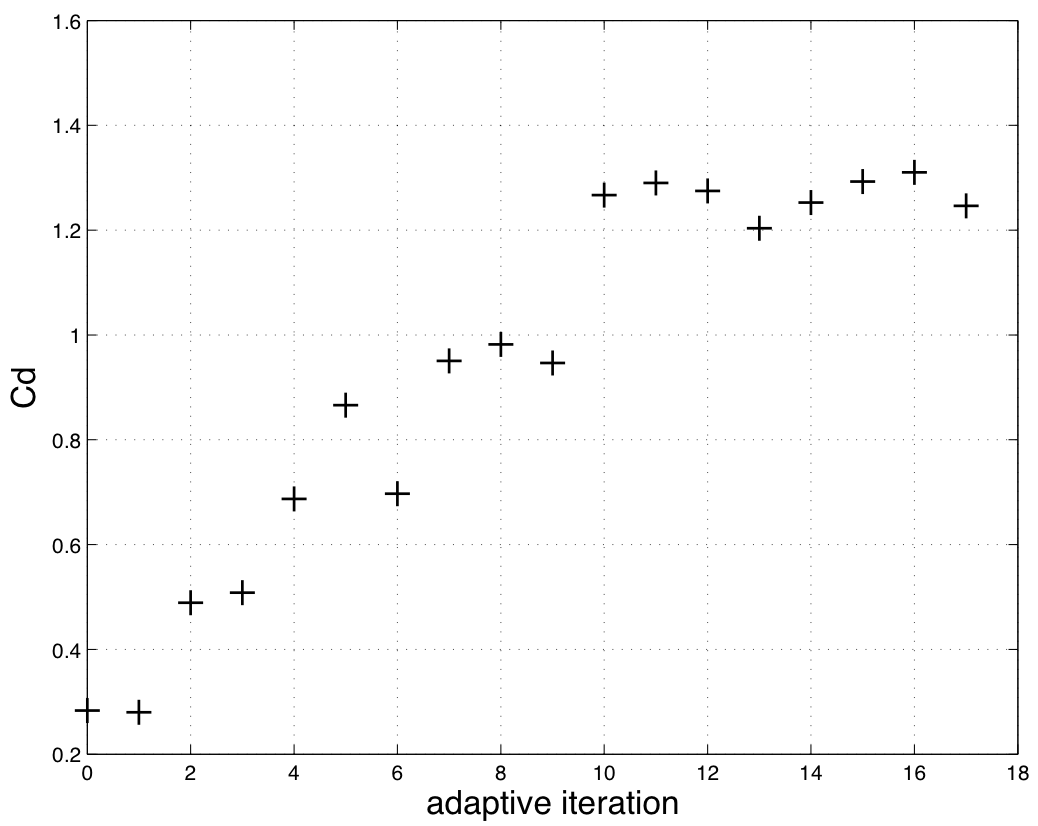
\includegraphics[height=5.4cm]{unfinished/hoffman-1/png/fig1a.png}
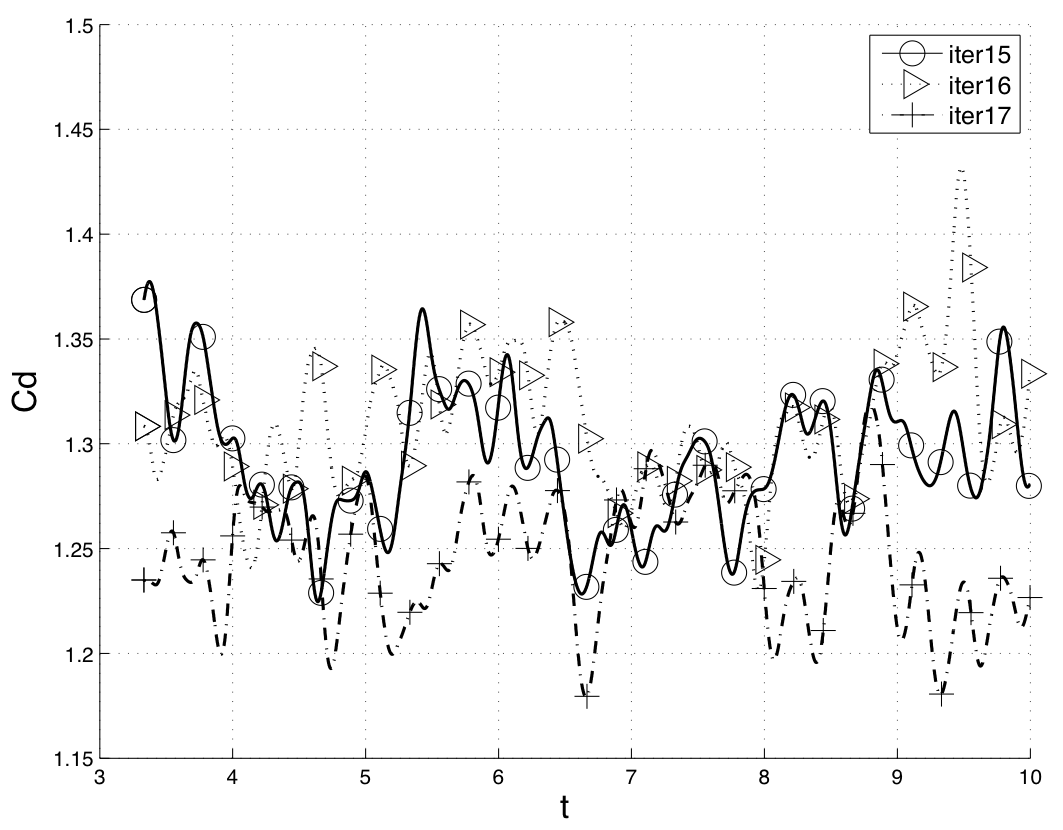
\includegraphics[height=5.4cm]{unfinished/hoffman-1/png/fig1b.png}
\caption{Flow around a cube: convergence of the drag coefficient under mesh refinement.}
\label{fig:cube1}
\end{figure}

\begin{figure}
\centering
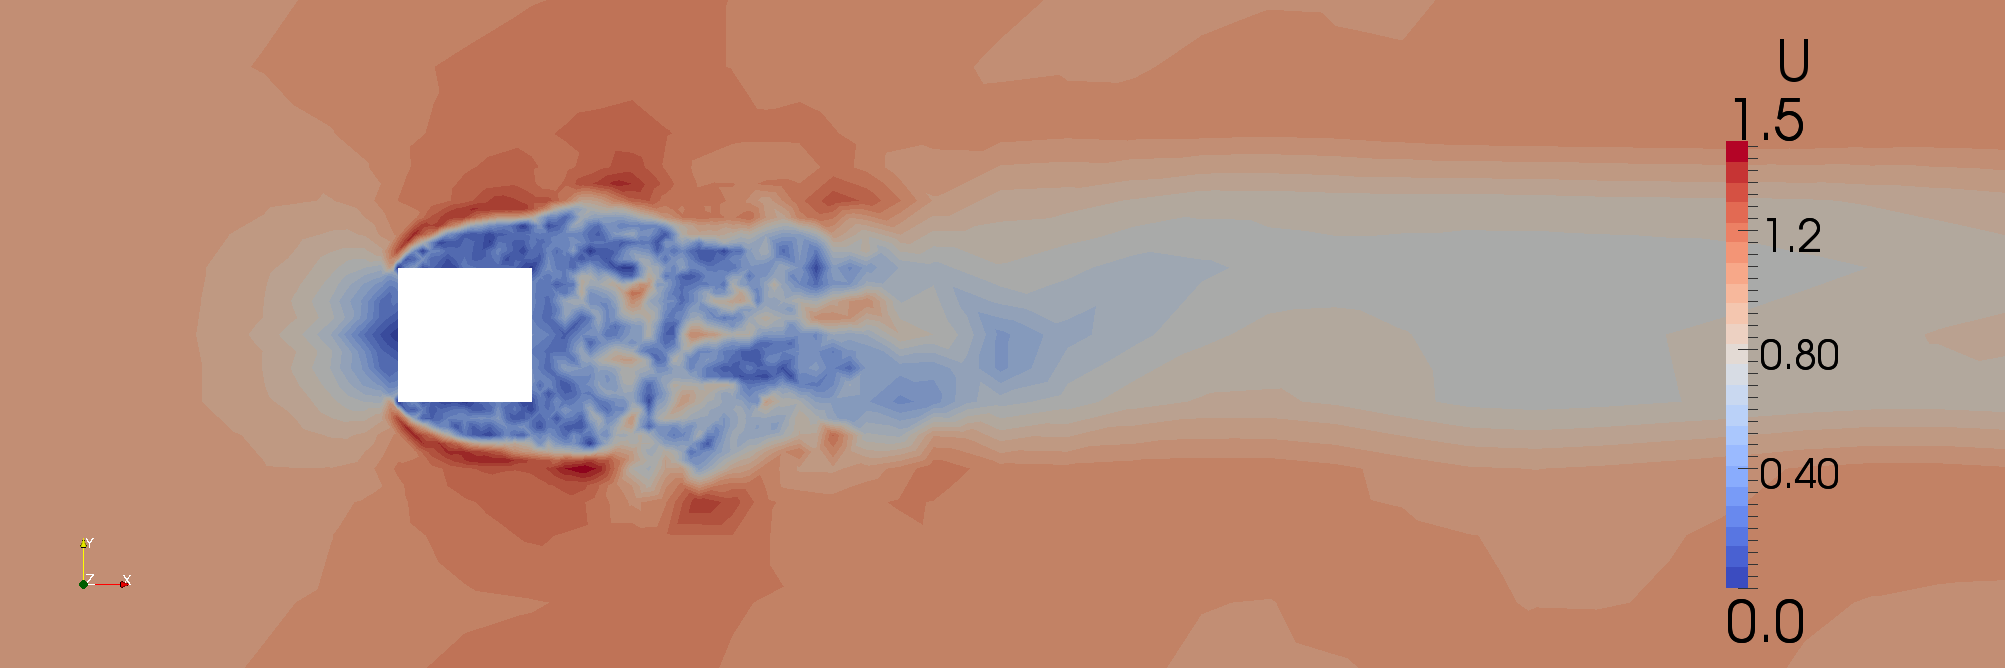
\includegraphics[width=11cm]{unfinished/hoffman-1/png/fig2b.png}

\medskip

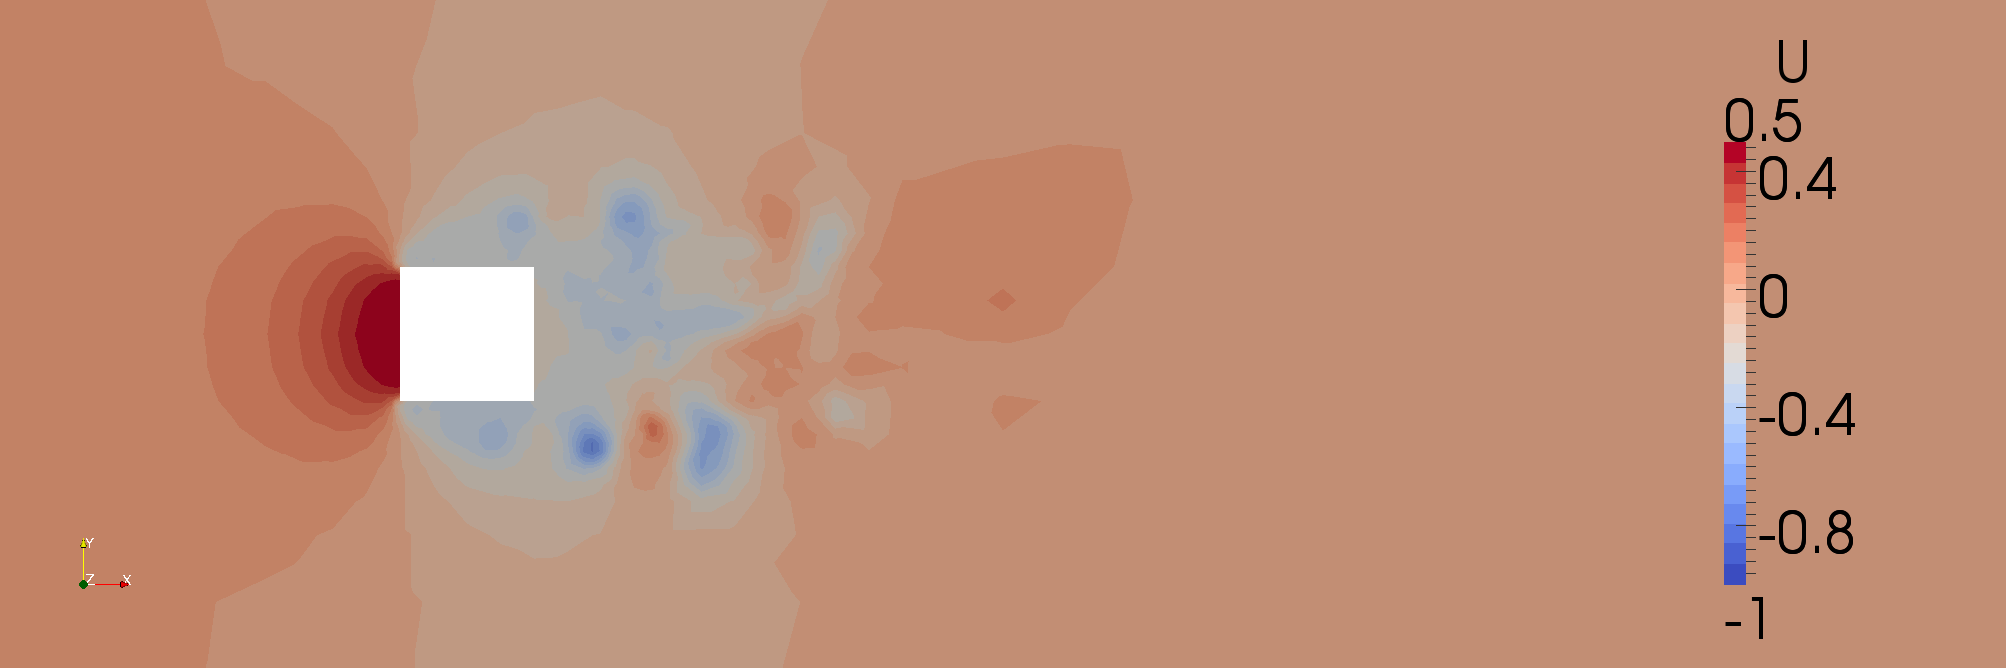
\includegraphics[width=11cm]{unfinished/hoffman-1/png/fig2c.png}
\caption{Flow around a cube: snapshots of velocity (upper) and pressure (lower) for the finest mesh.}
\label{fig:cube2}
\end{figure}

\begin{figure}
\centering
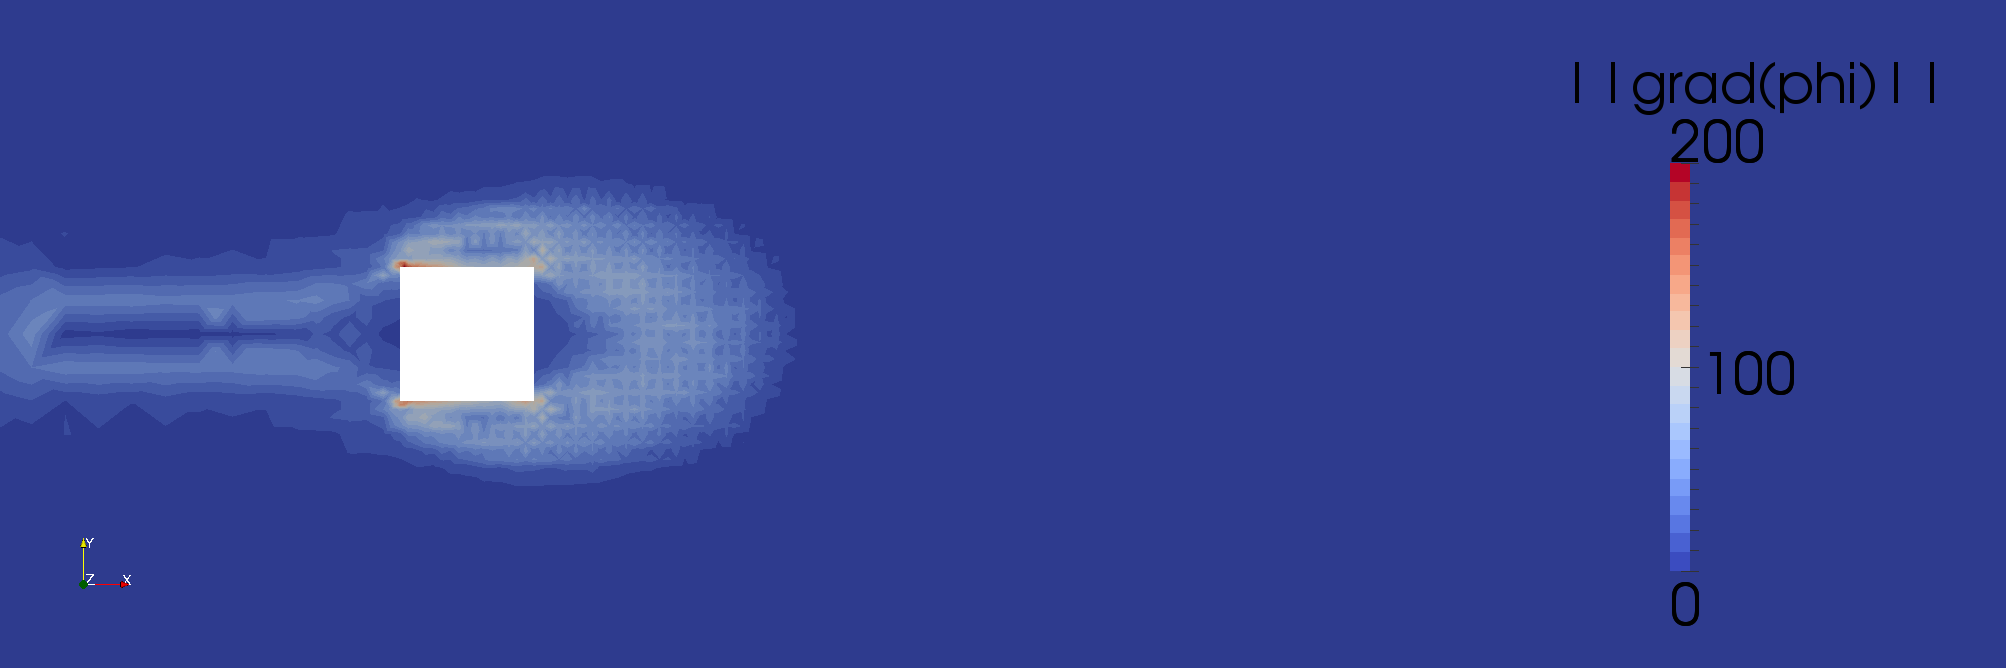
\includegraphics[width=11cm]{unfinished/hoffman-1/png/fig3a.png}

\medskip

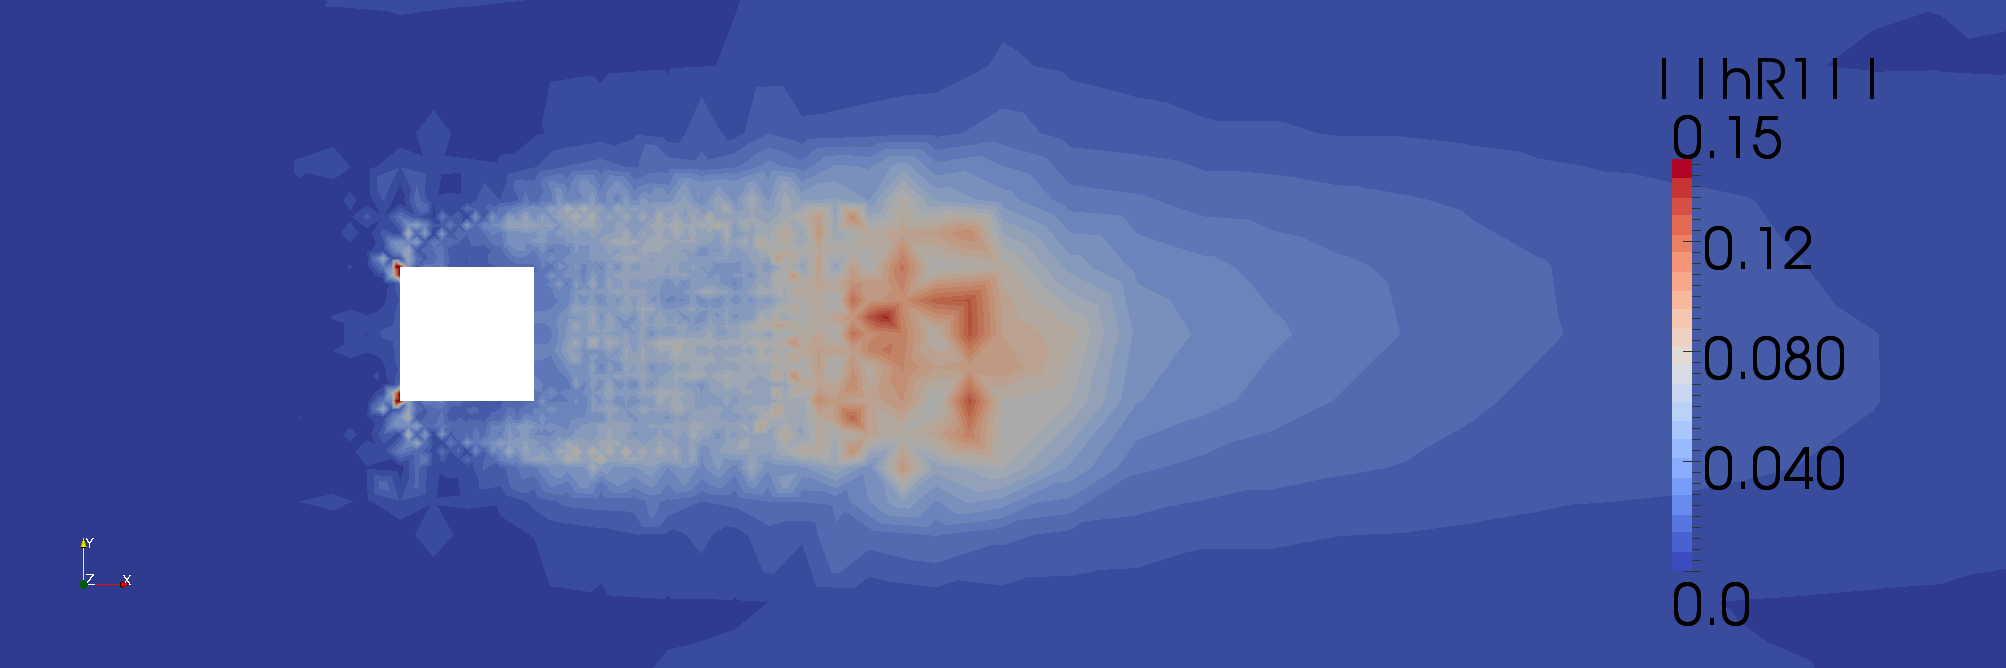
\includegraphics[width=11cm]{unfinished/hoffman-1/png/fig3b.png}
\caption{Flow around a cube: gradient of dual velocity (upper) and local error (lower), on a mesh after 16 adaptive mesh refinements.}
\label{fig:cube3}
\end{figure}


\subsection{Turbulent flow separation}

In Unicorn, the effect of turbulent boundary layers is modeled by a skin friction wall shear stress model, described above. This model has one parameter $\beta$, which is related to the skin friction stress (following \cite{Schumann1975} a skin friction stress normalized by a velocity). Higher Reynolds number is modeled by a smaller $\beta$, based on experimental observation that the skin friction (coefficient) decrease with increasing $Re$.

To estimate the dependence of the computational result on $\beta$, in \cite{HoffmanJansson2009} a computational study carried out using Unicorn, where the drag force of a circular cylinder is computed adaptively based on a posteriori error estimation. In particular, the phenomenon of drag crisis is targeted, characterized by a sudden drop in the non-dimensional drag coefficient for a cylinder for $Re$ increasing beyond a critical size of about $10^5$. By decreasing the skin friction parameter $\beta$, modeling an increasing $Re$, the drag crisis scenario is reproduced using Unicorn, in agreement with the high $Re$ experimental data available in the literature \cite{Zdravkovich2003}. In particular, the drag coefficient drops to a level found in experiments after drag crisis, and 3D so called cell structures develop in the form of streamwise vorticity, also reported in the literature \cite{Zdravkovich2003}.
For vanishing skin friction the flow approaches a state independent of the skin friction parameter, which thus corresponds to a free slip boundary condition, see Fig.\ref{fig:1}-\ref{fig:3}. Although controversial, this suggests a dominant inviscid separation mechanism independent of the boundary layer, investigated in \cite{HoffmanJohnson2008b,HoffmanJansson2009}.


\begin{figure}
\centering
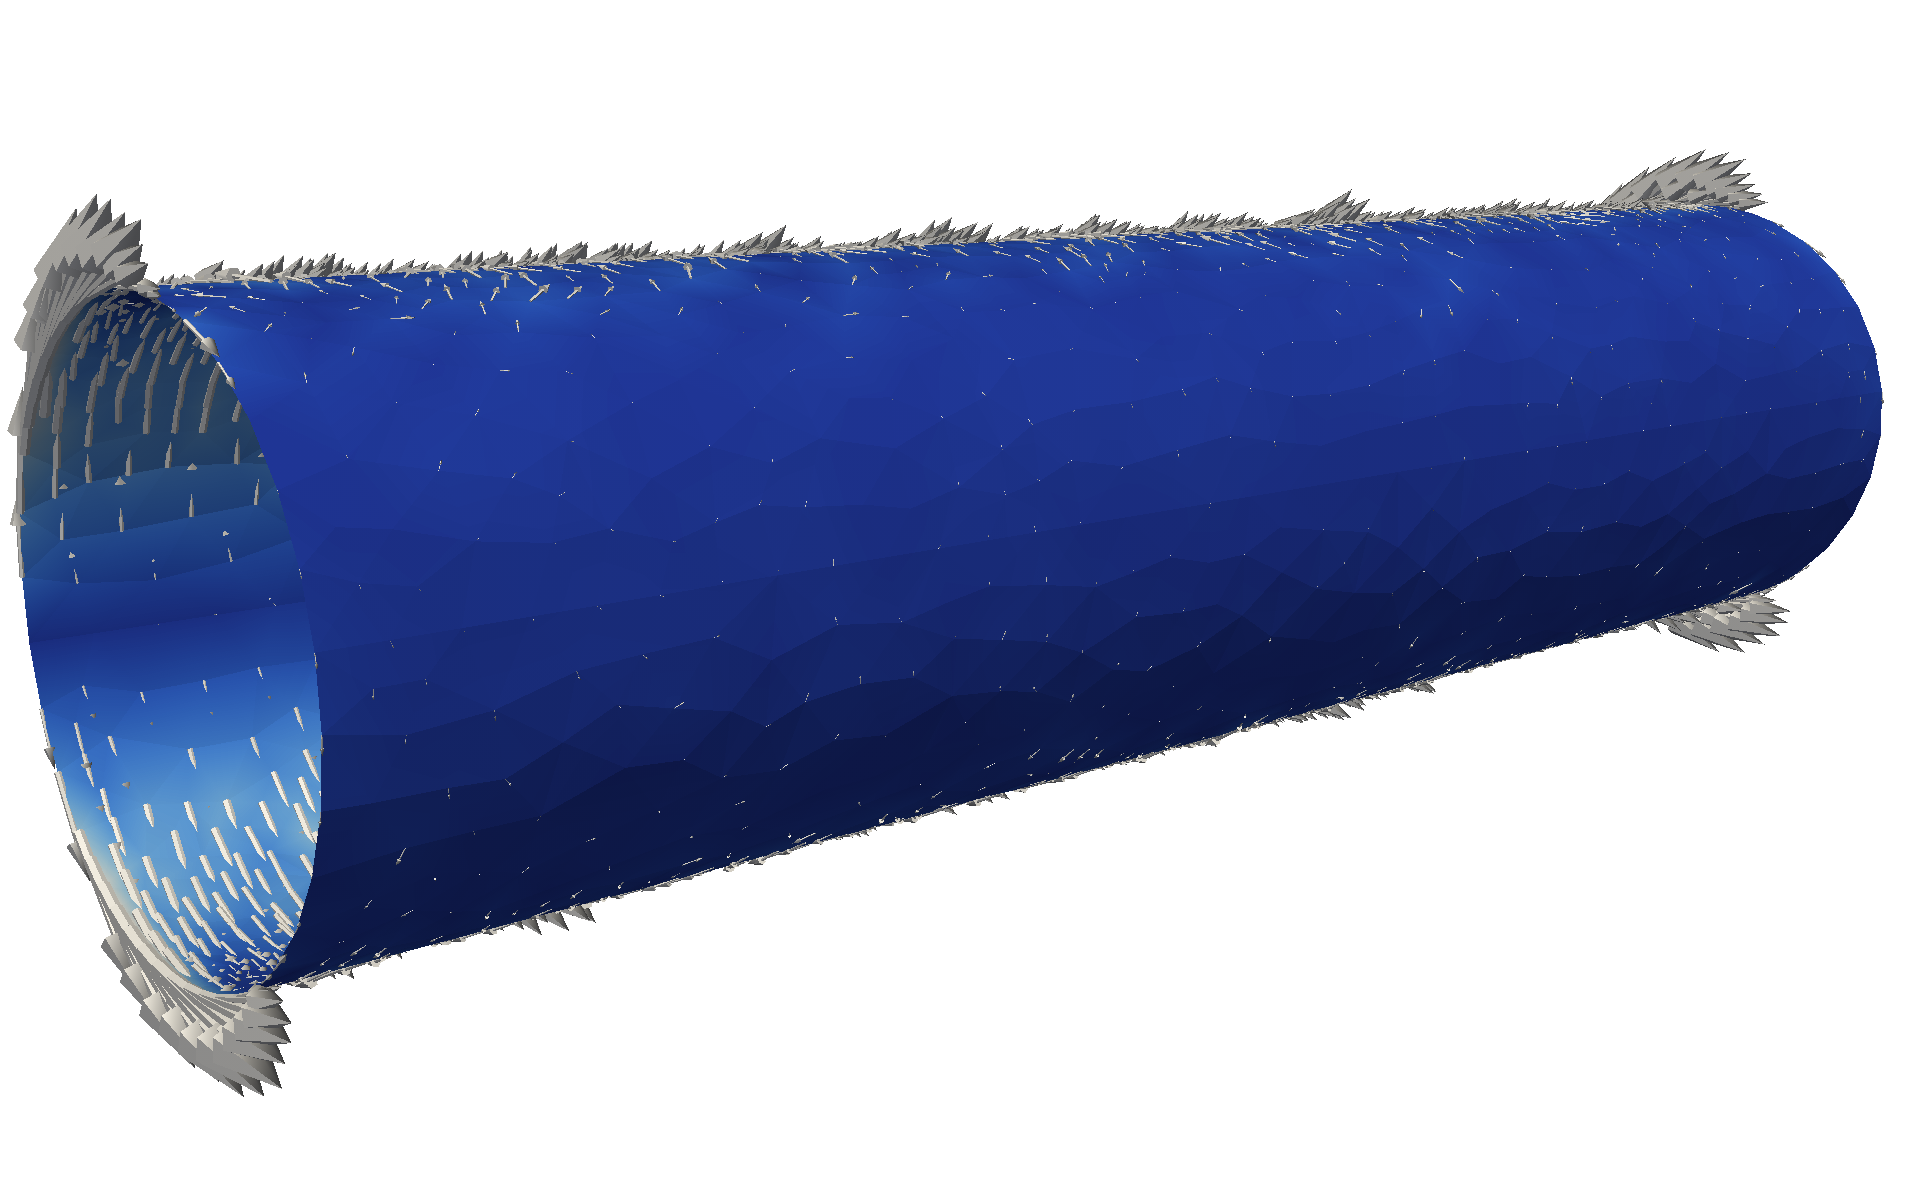
\includegraphics[height=4cm]{unfinished/hoffman-1/png/Hoffman_fig2a.png}
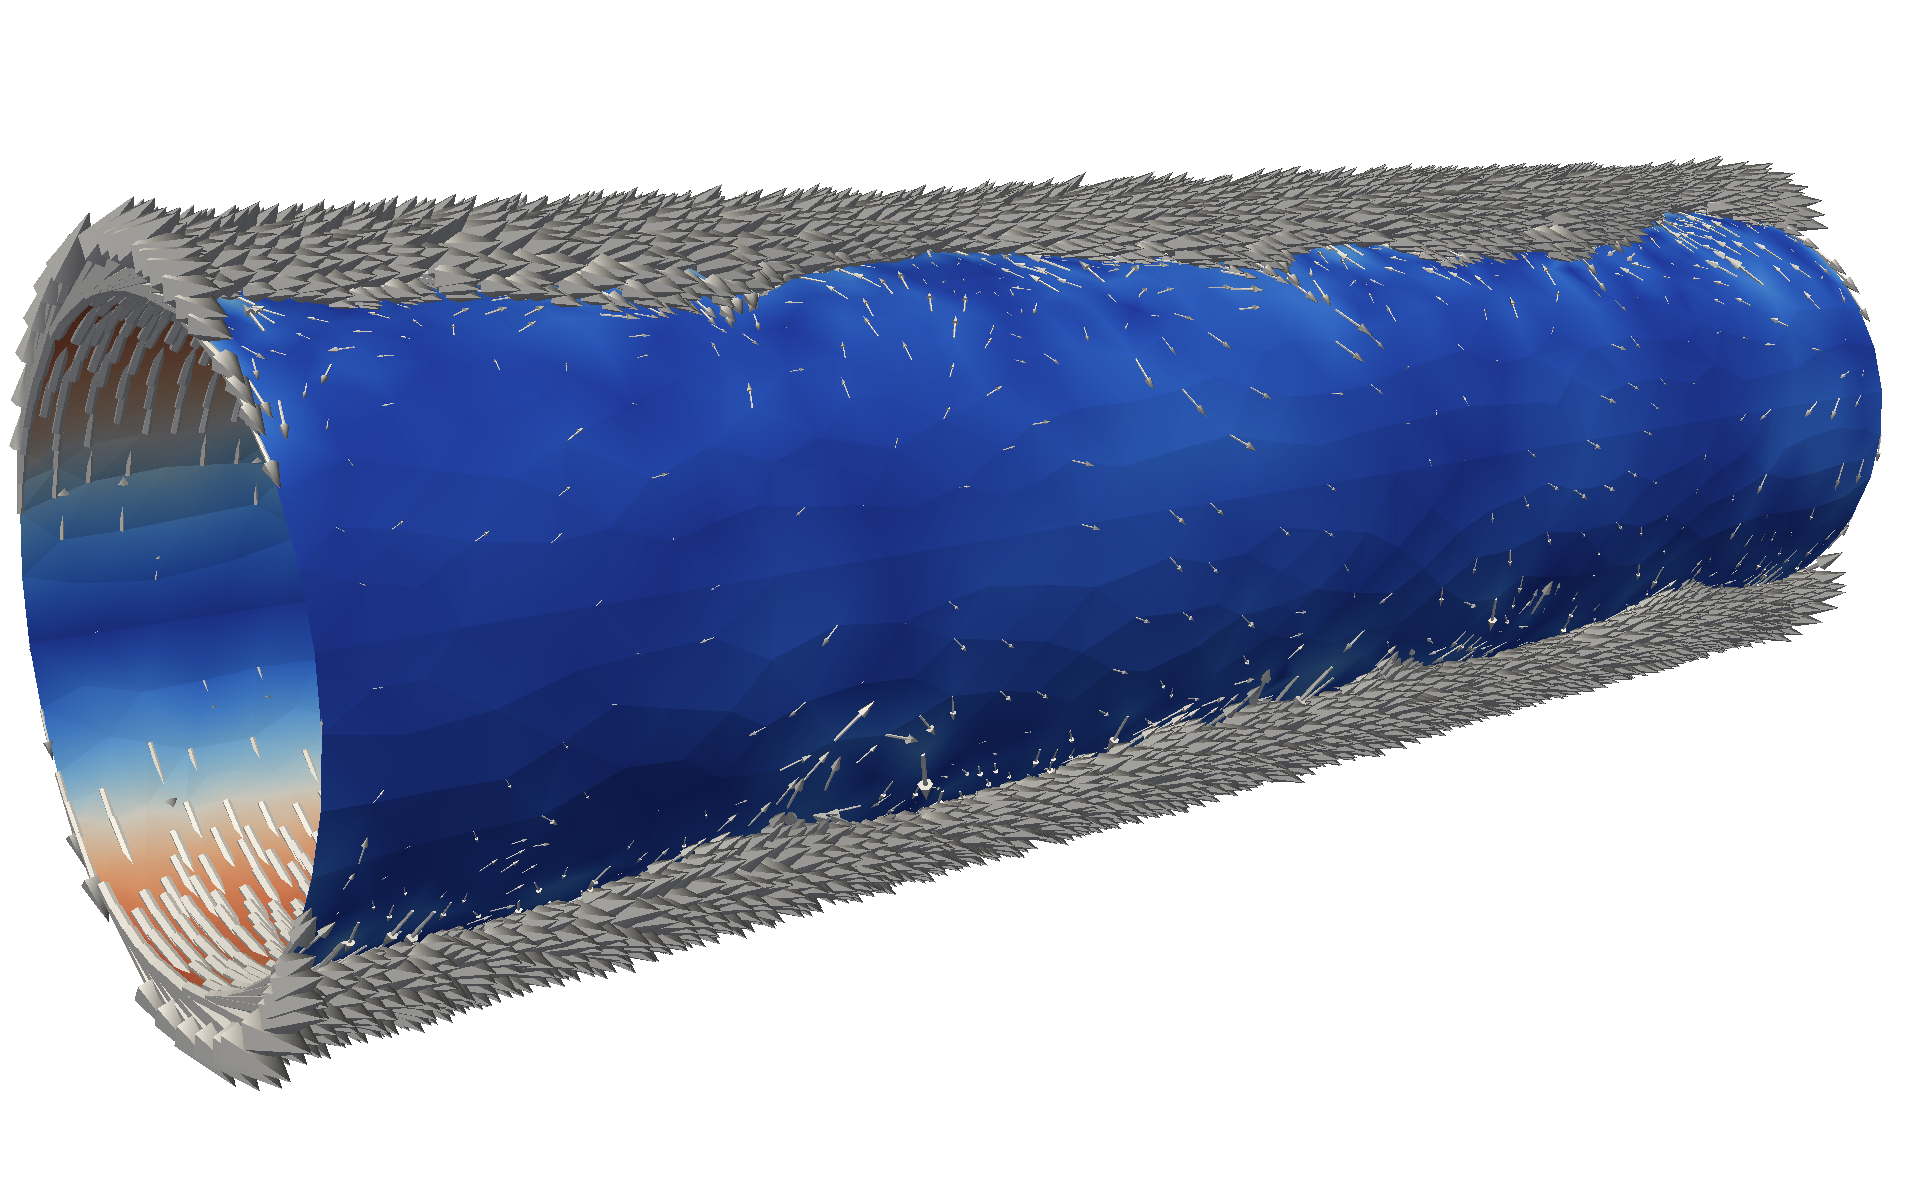
\includegraphics[height=4cm]{unfinished/hoffman-1/png/Hoffman_fig2b.png}
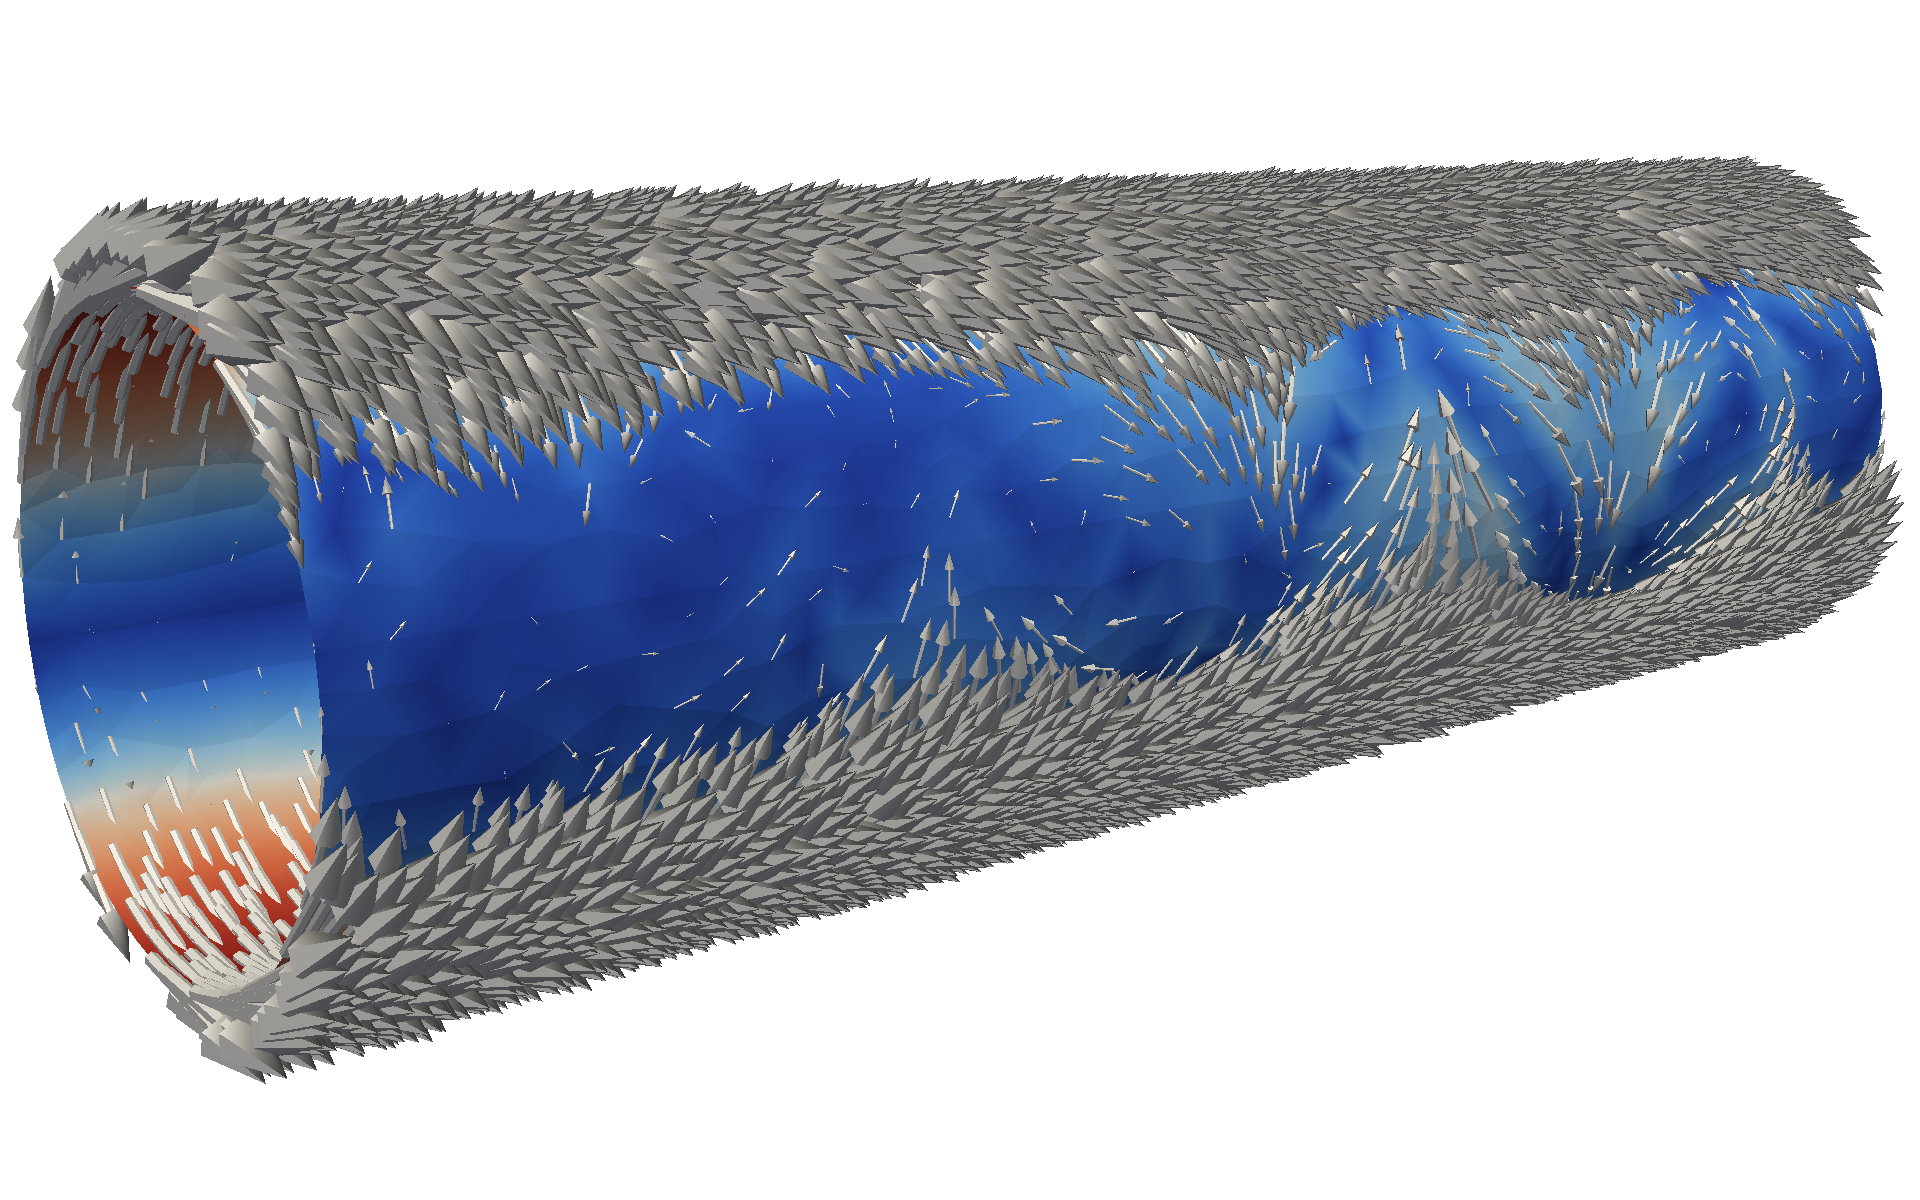
\includegraphics[height=4cm]{unfinished/hoffman-1/png/Hoffman_fig2c.png}
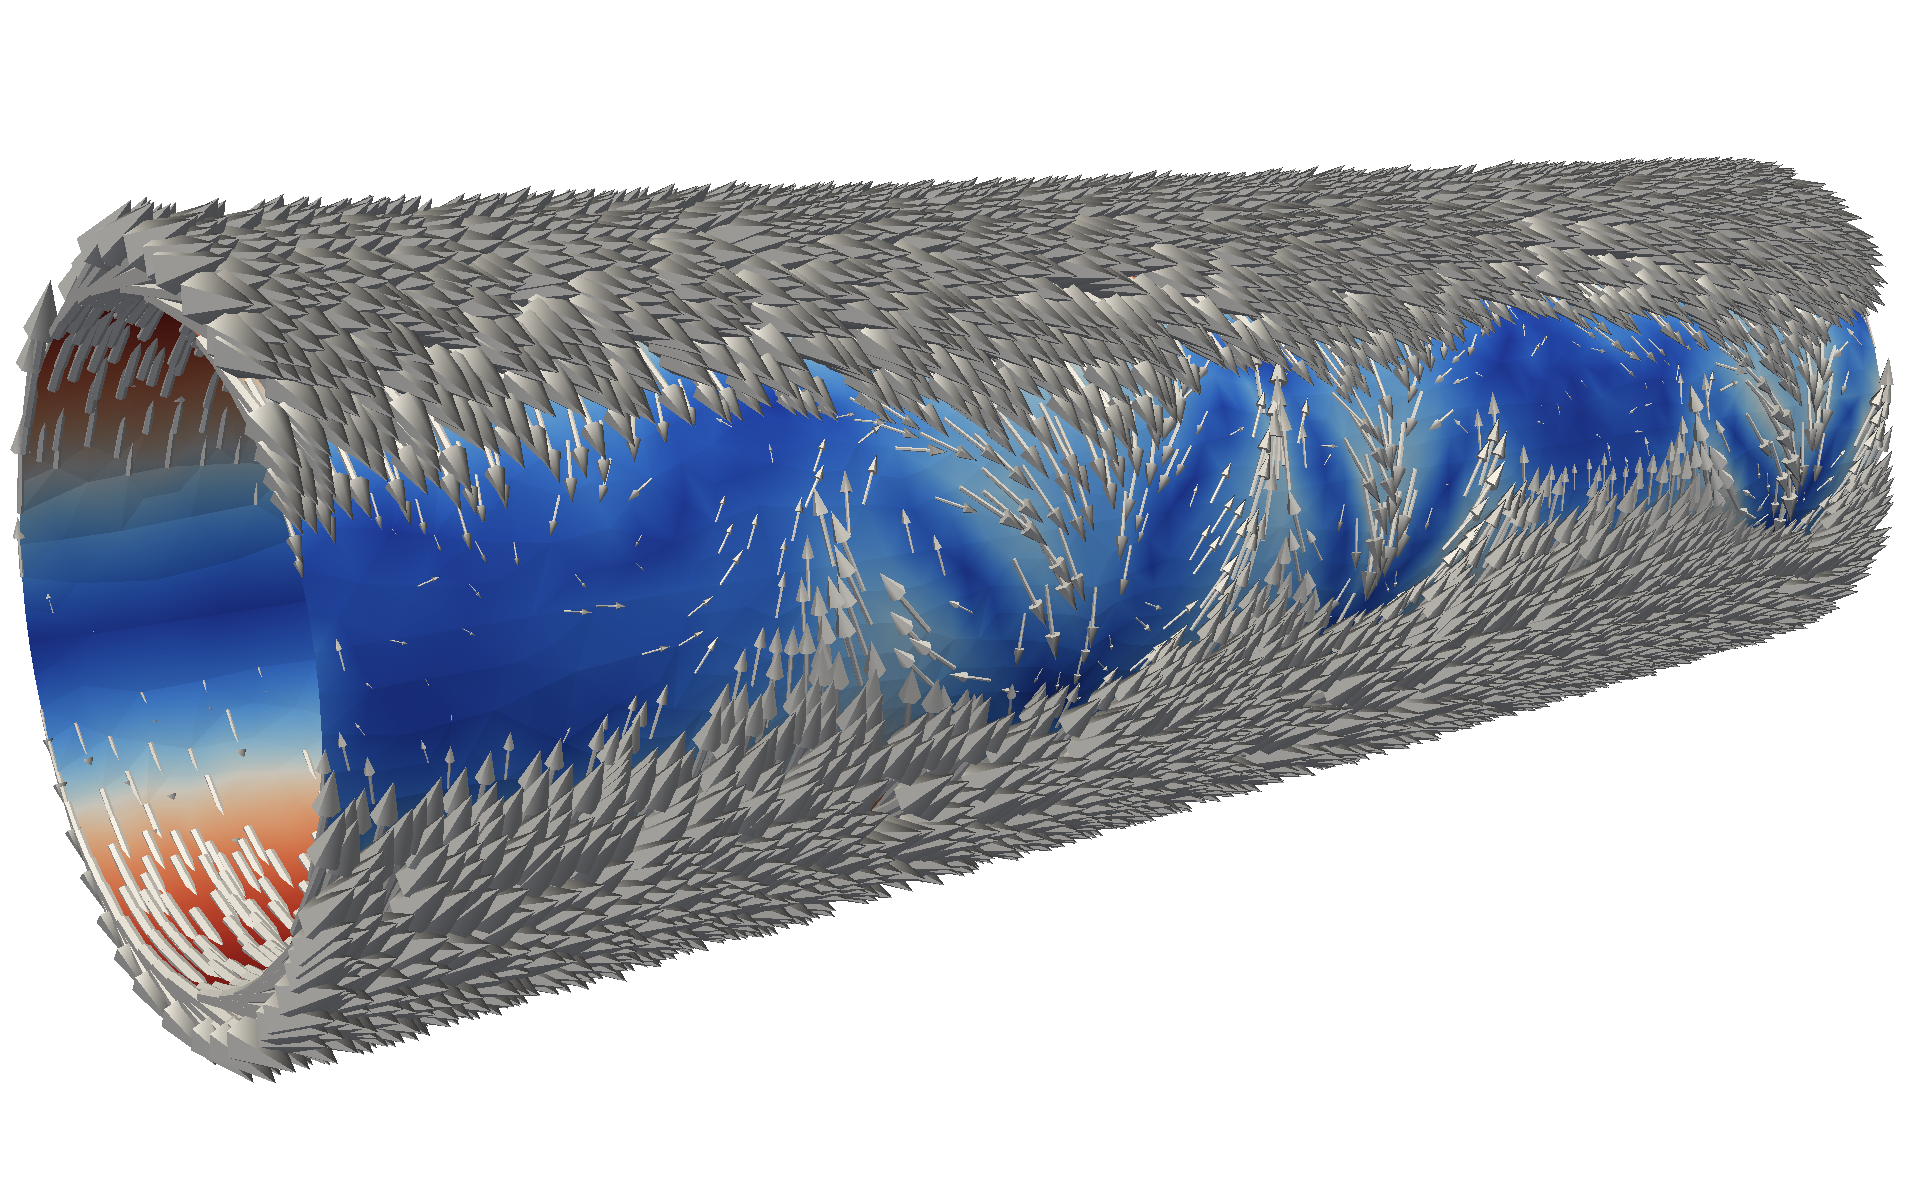
\includegraphics[height=4cm]{unfinished/hoffman-1/png/Hoffman_fig2d.png}
\caption{Turbulent flow separation  \cite{HoffmanJansson2009}: velocity vectors at surface of cylinder; for $\beta = 10^{-1}$, $\beta = 10^{-2}$, $\beta = 10^{-3}$ and $\beta = 0$ (from upper left to bottom right).}
\label{fig:1}
\end{figure}

\begin{figure}
\centering
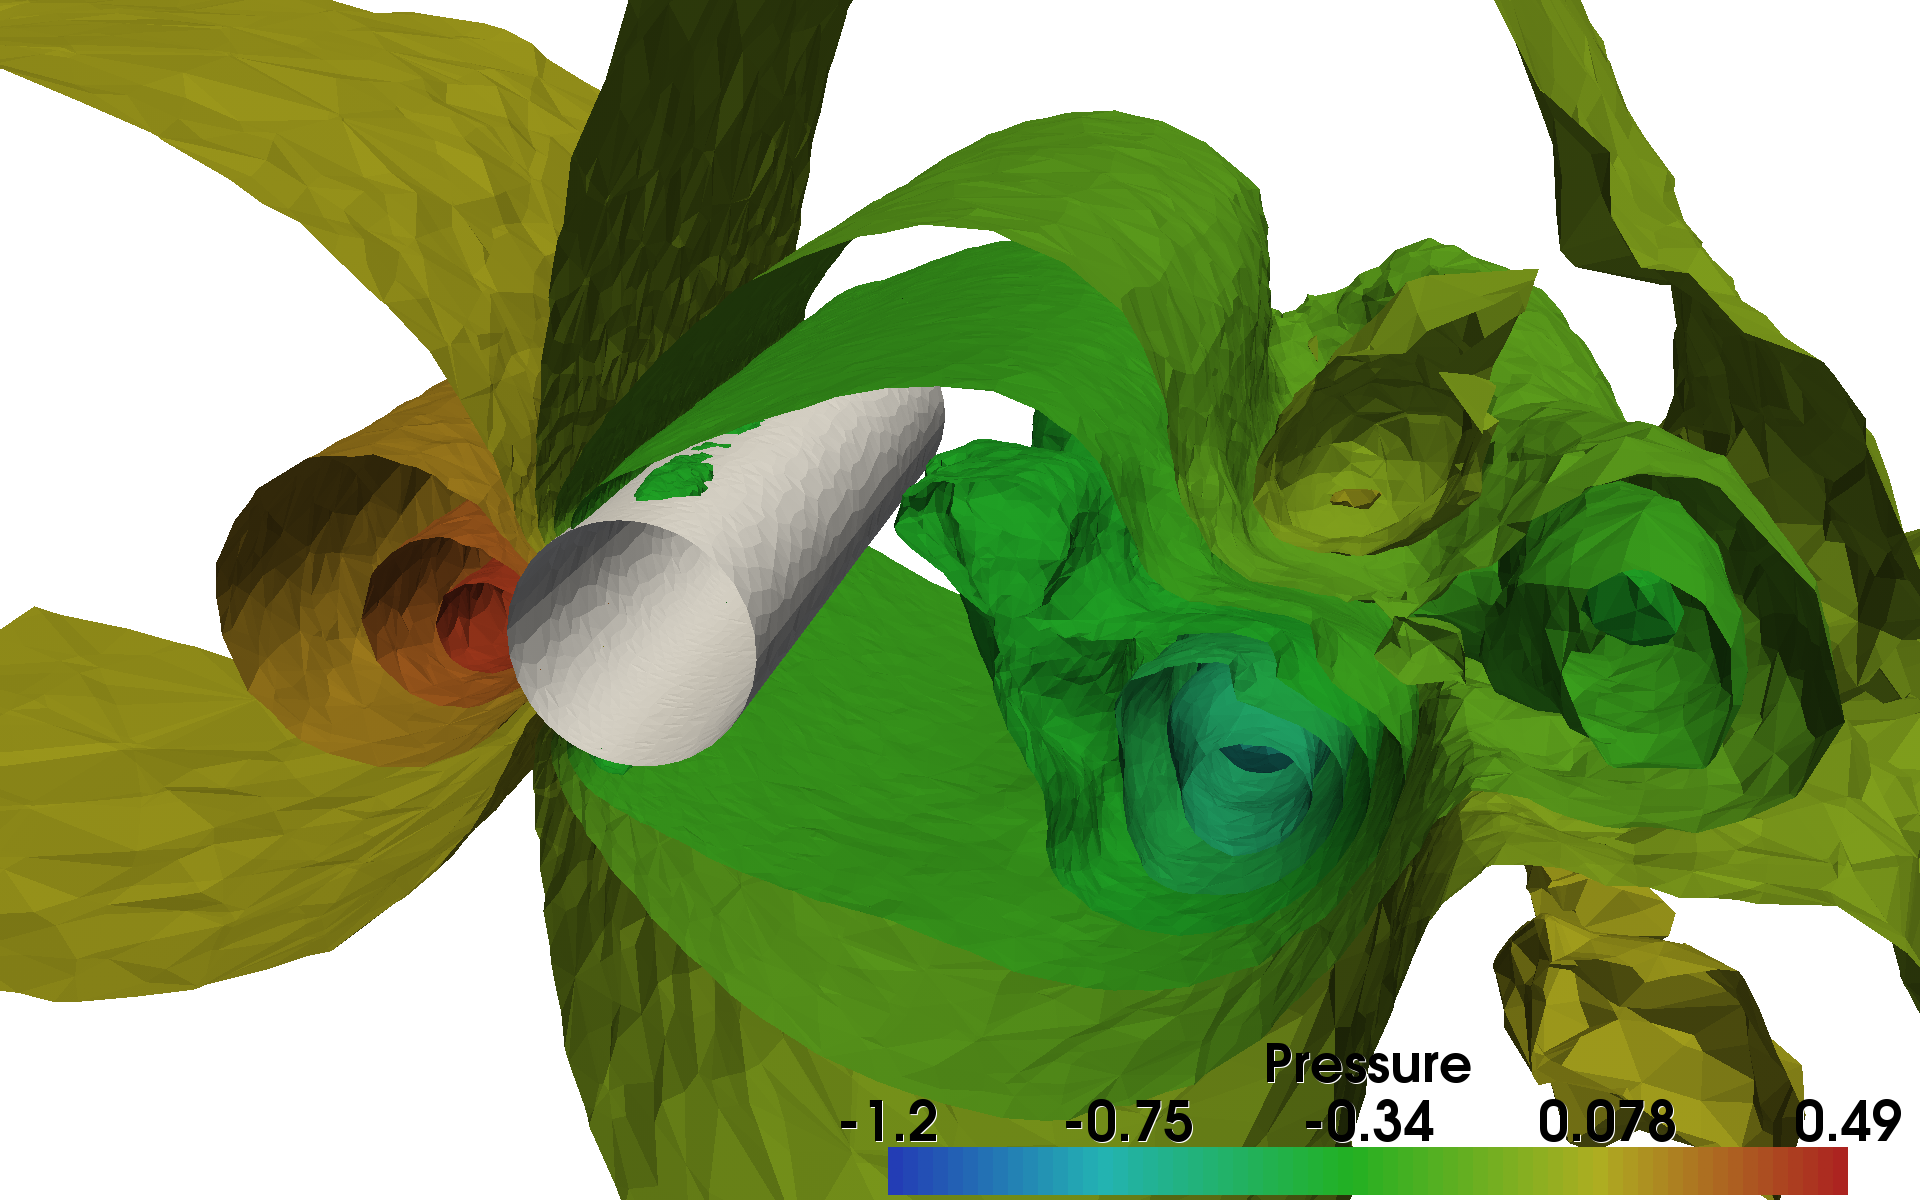
\includegraphics[height=4cm]{unfinished/hoffman-1/png/Hoffman_fig3a.png}
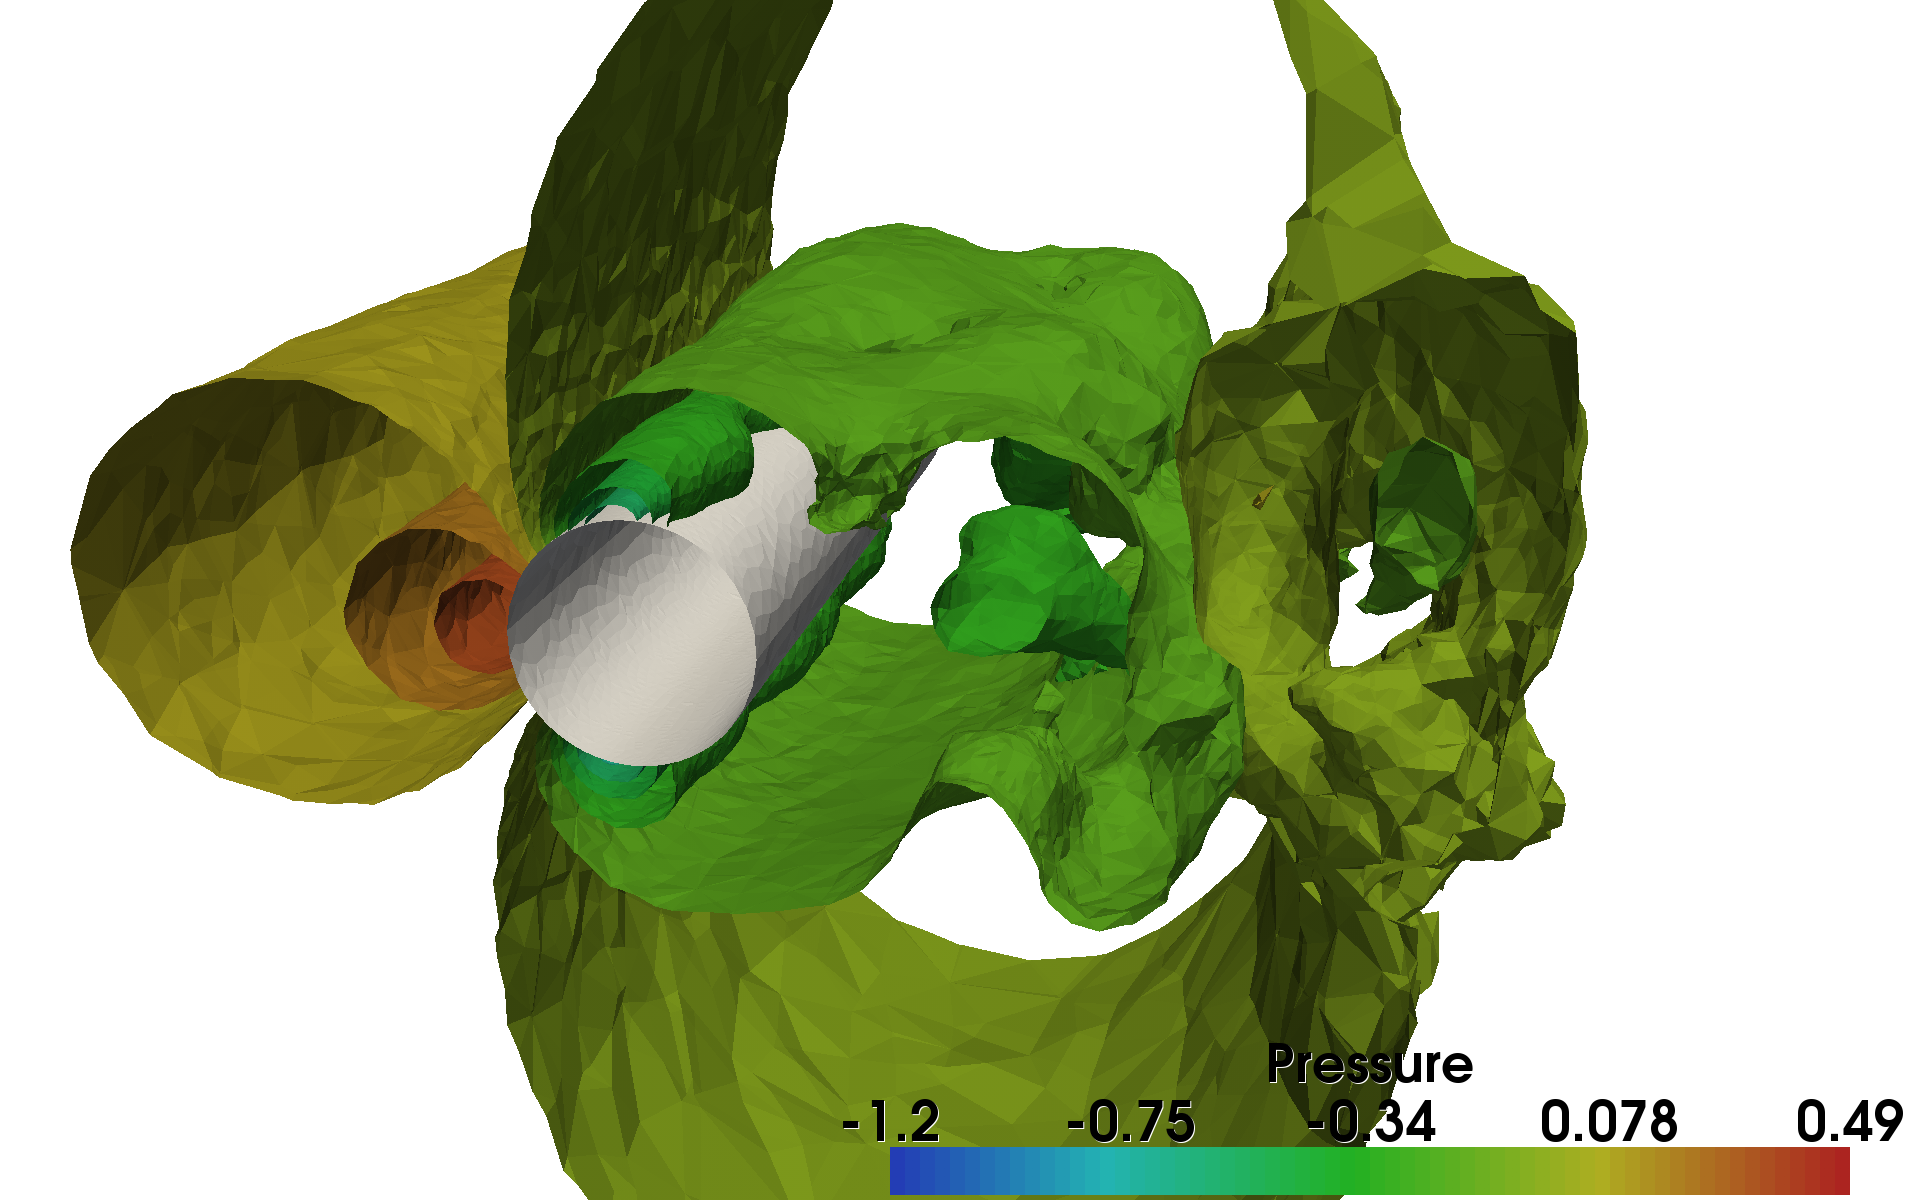
\includegraphics[height=4cm]{unfinished/hoffman-1/png/Hoffman_fig3b.png}
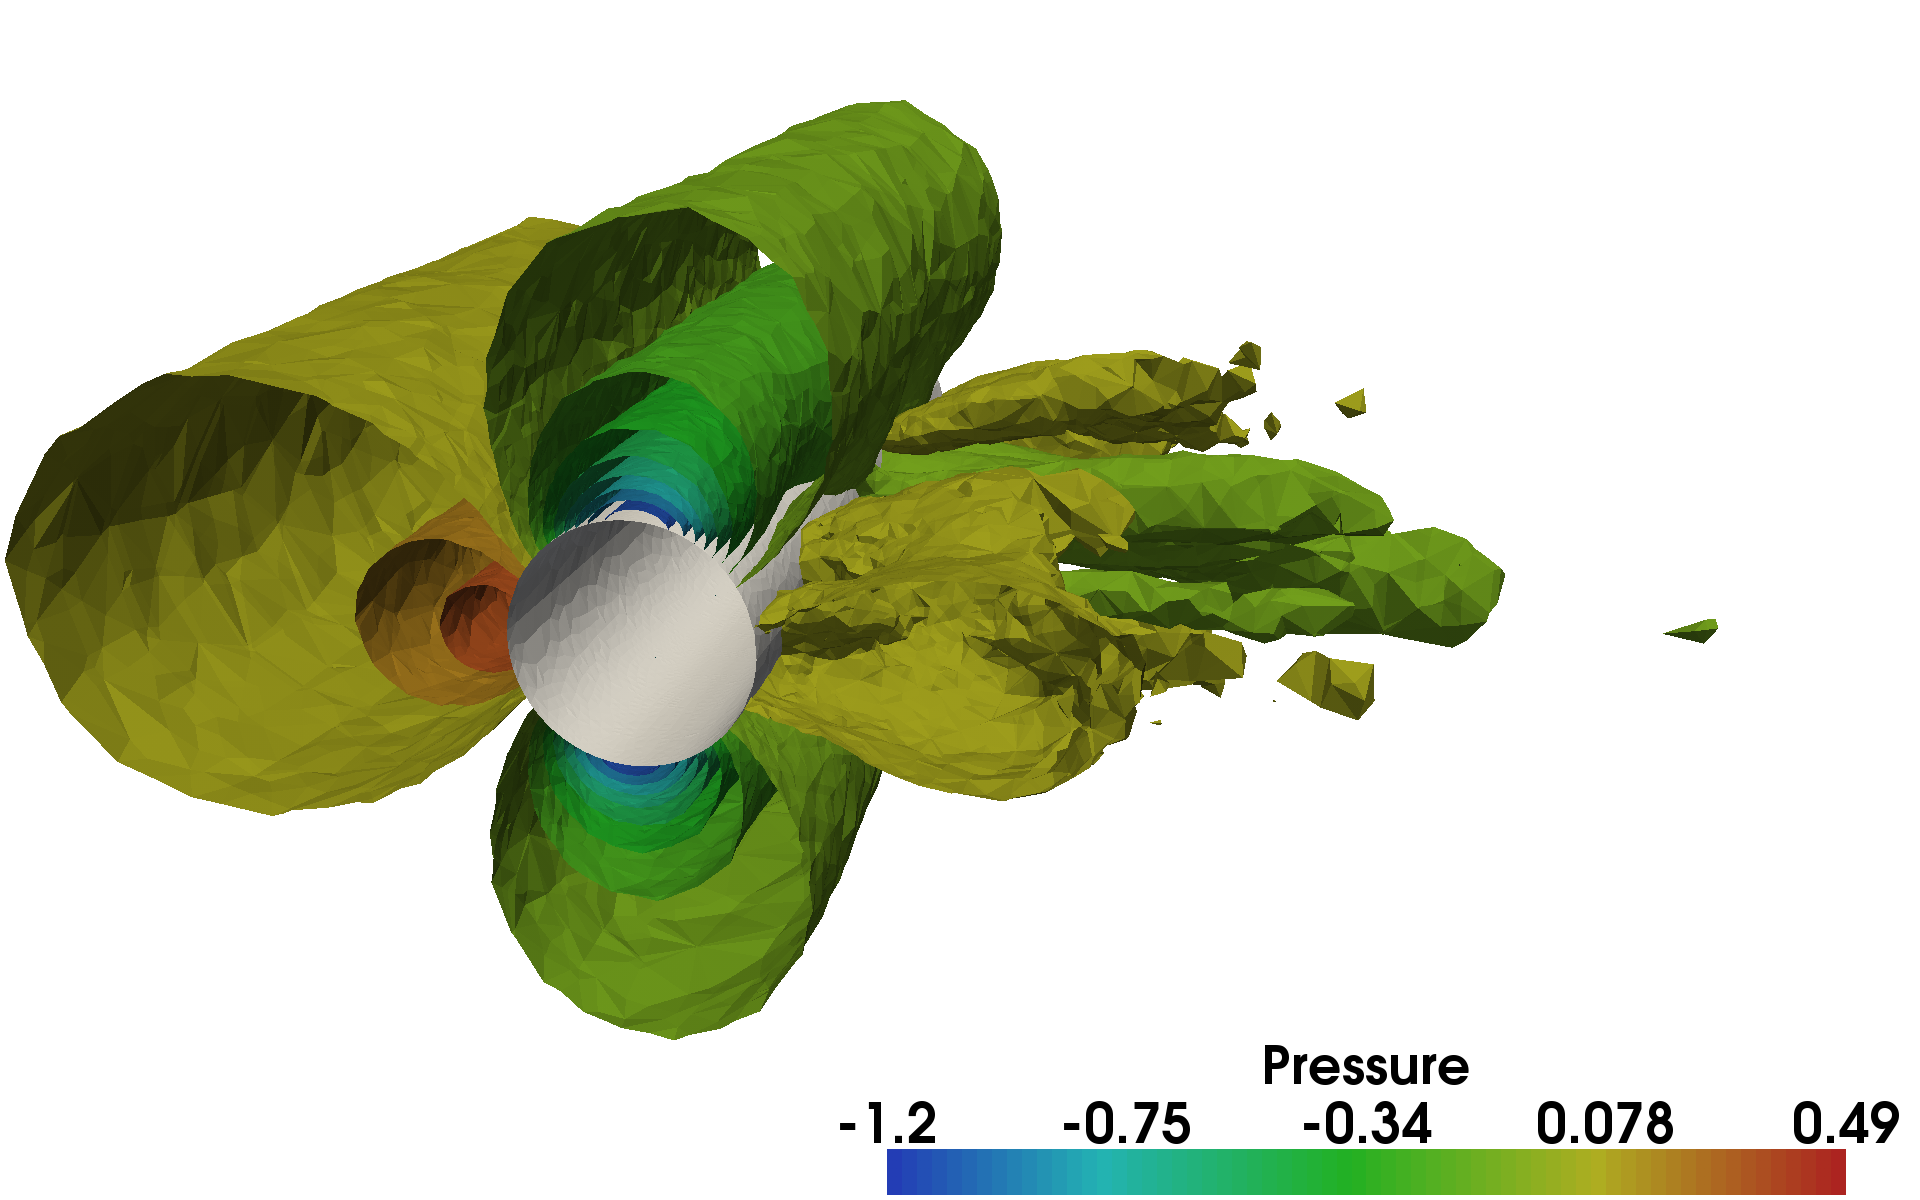
\includegraphics[height=4cm]{unfinished/hoffman-1/png/Hoffman_fig3c.png}
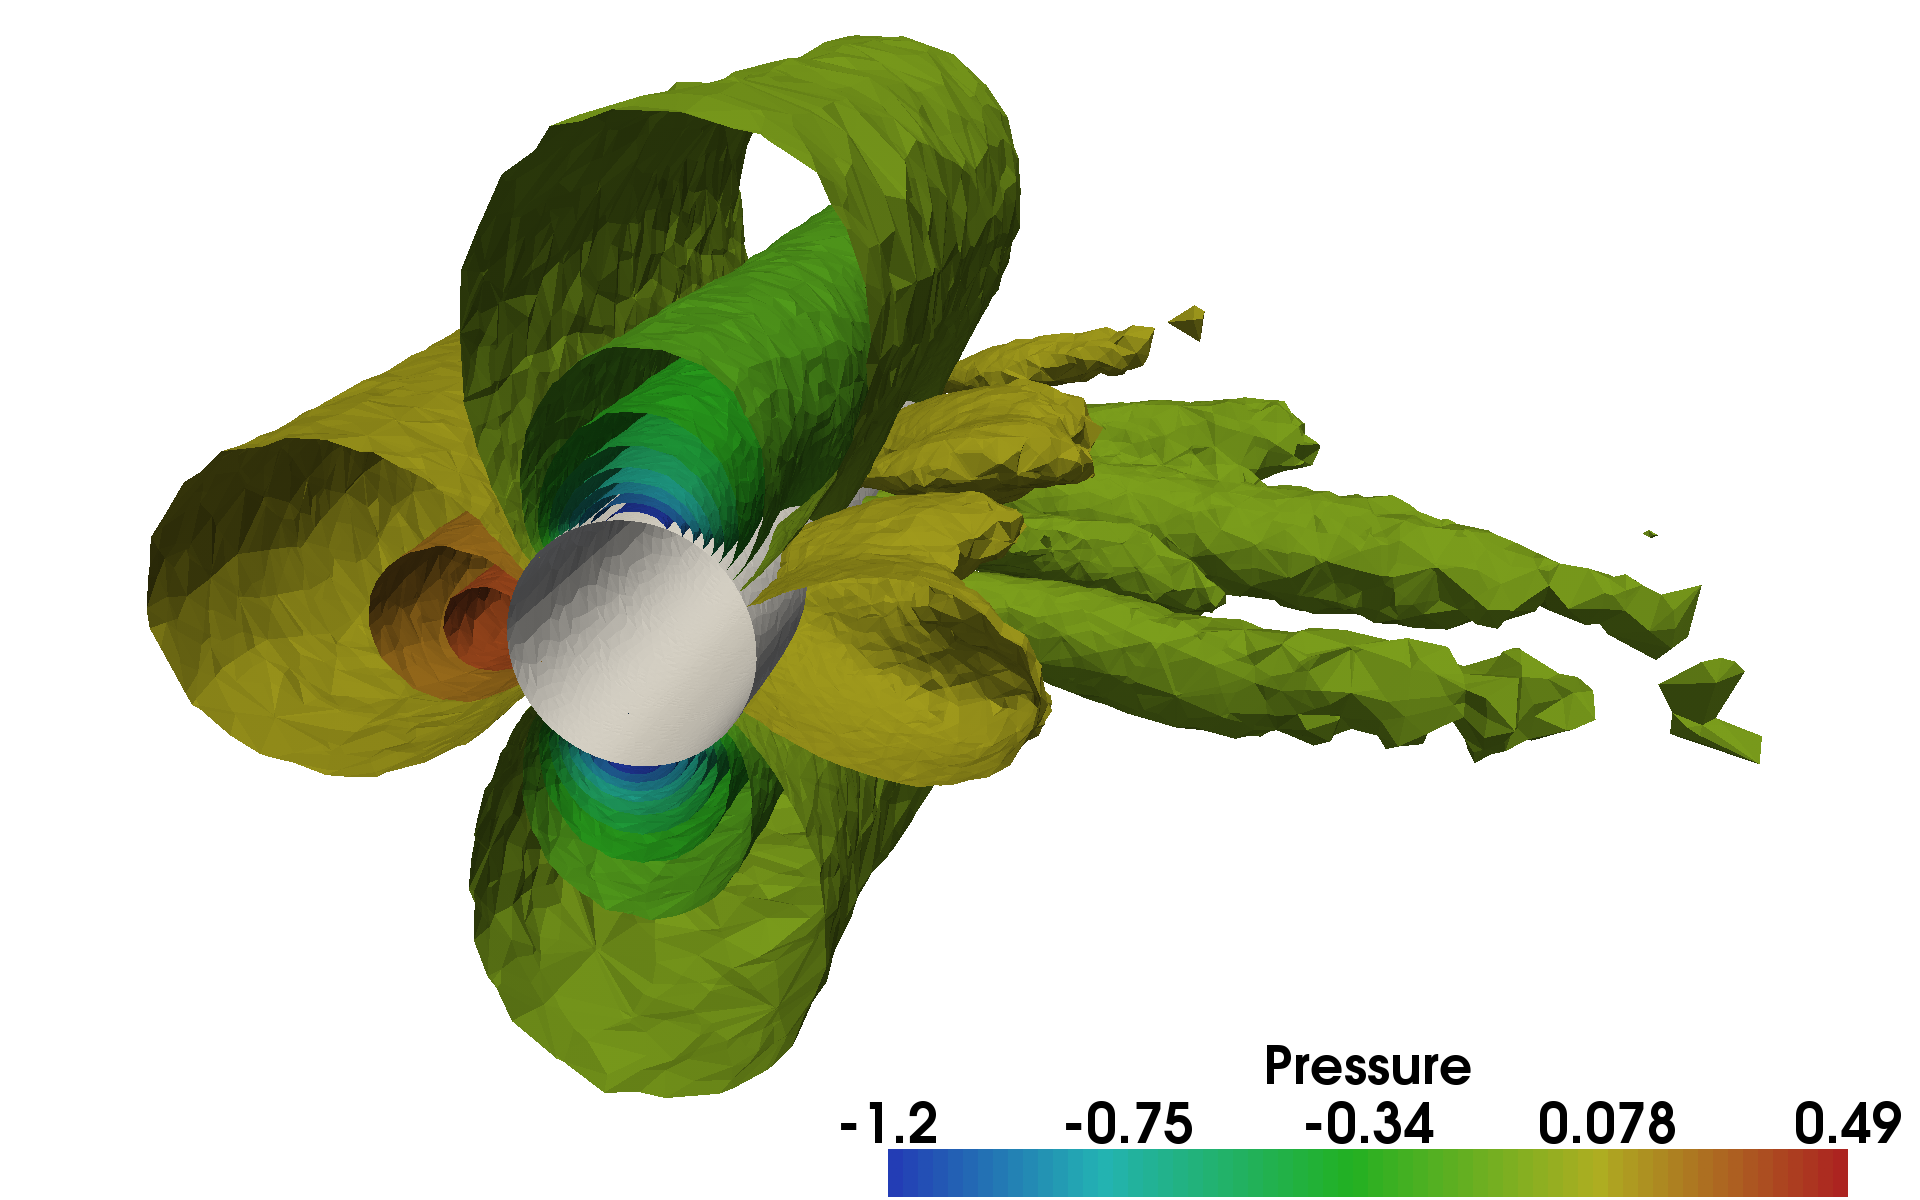
\includegraphics[height=4cm]{unfinished/hoffman-1/png/Hoffman_fig3d.png}
\caption{Turbulent flow separation \cite{HoffmanJansson2009}: pressure isosurfaces; for $\beta = 10^{-1}$, $\beta = 10^{-2}$, $\beta = 10^{-3}$ and $\beta = 0$ (from upper left to bottom right).}
\label{fig:2}
\end{figure}

\begin{figure}
\centering
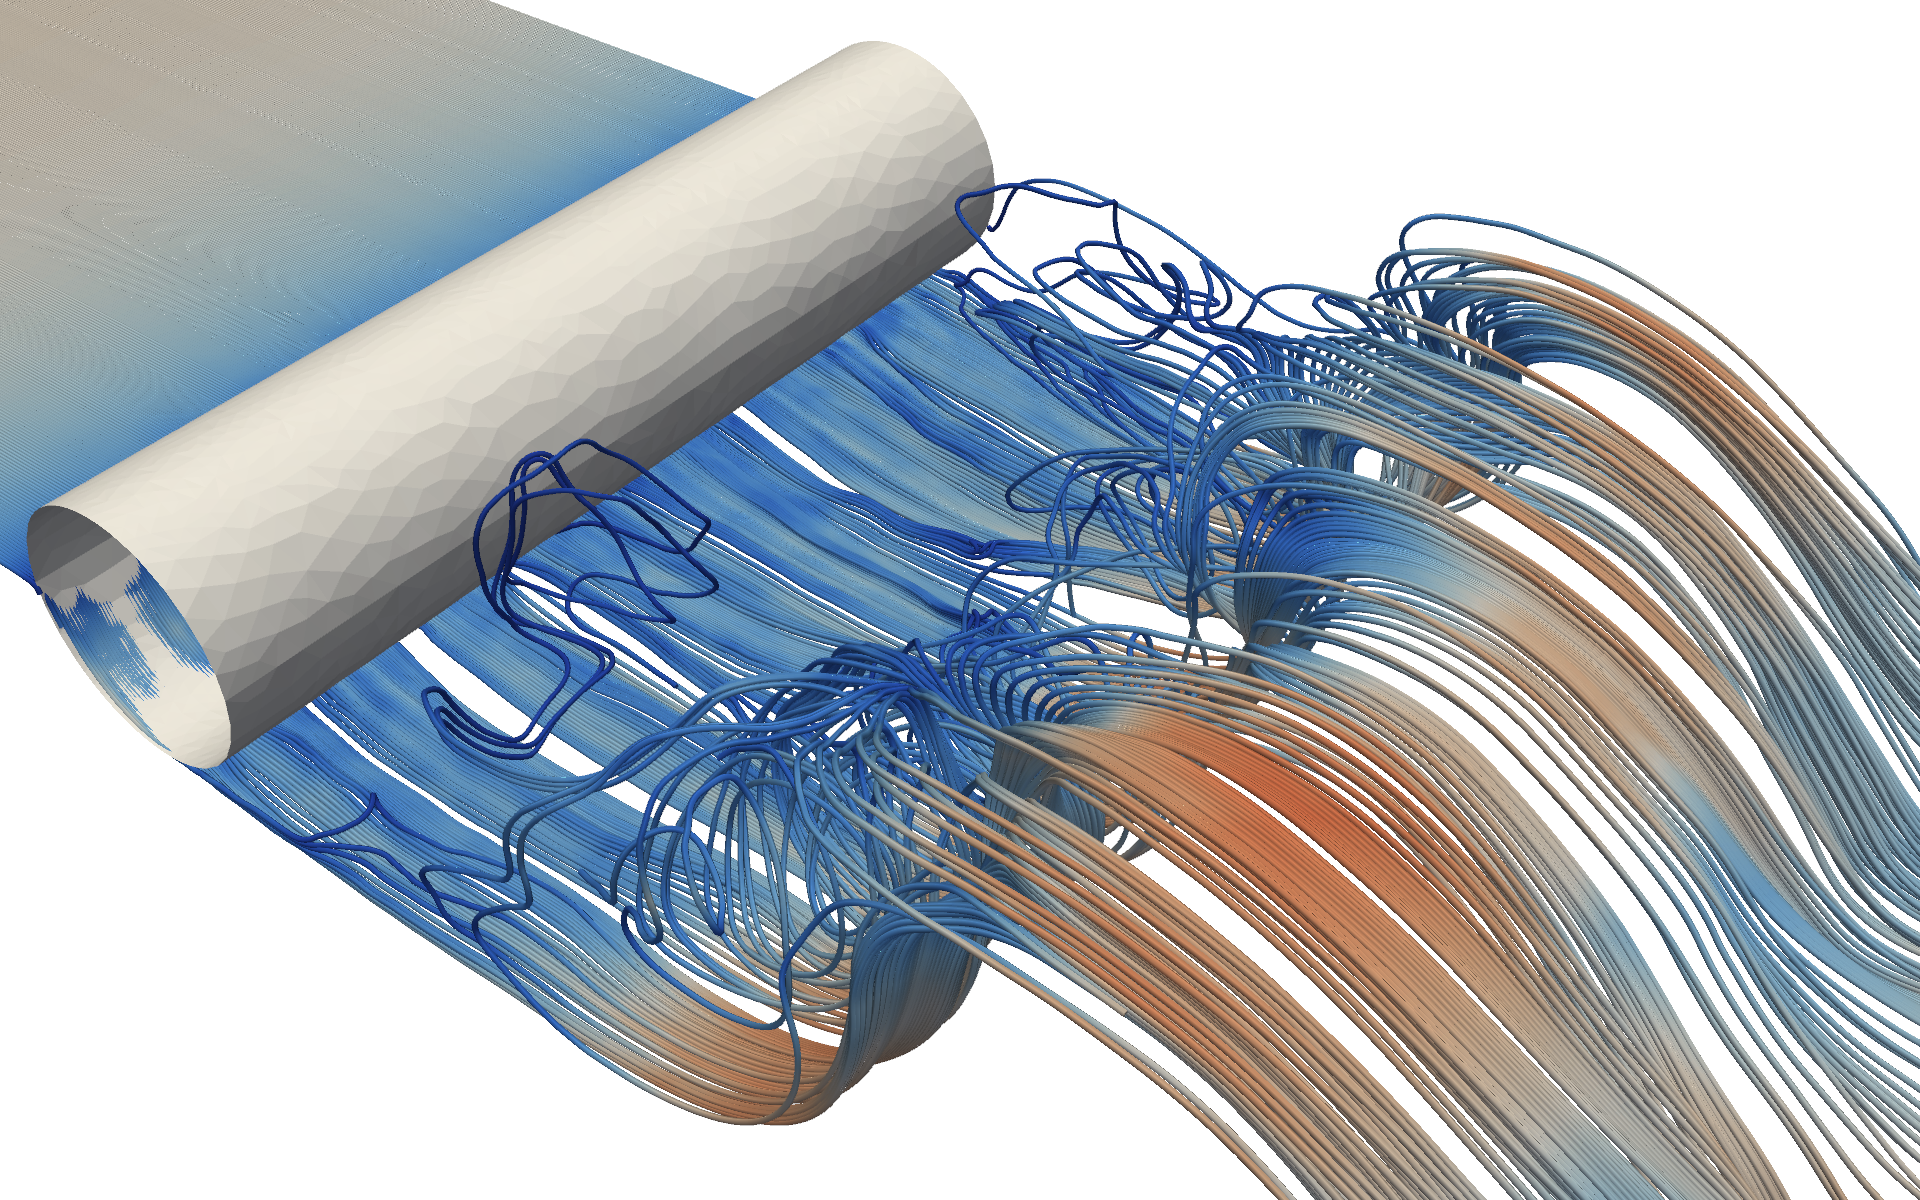
\includegraphics[height=4cm]{unfinished/hoffman-1/png/Hoffman_fig5a.png}
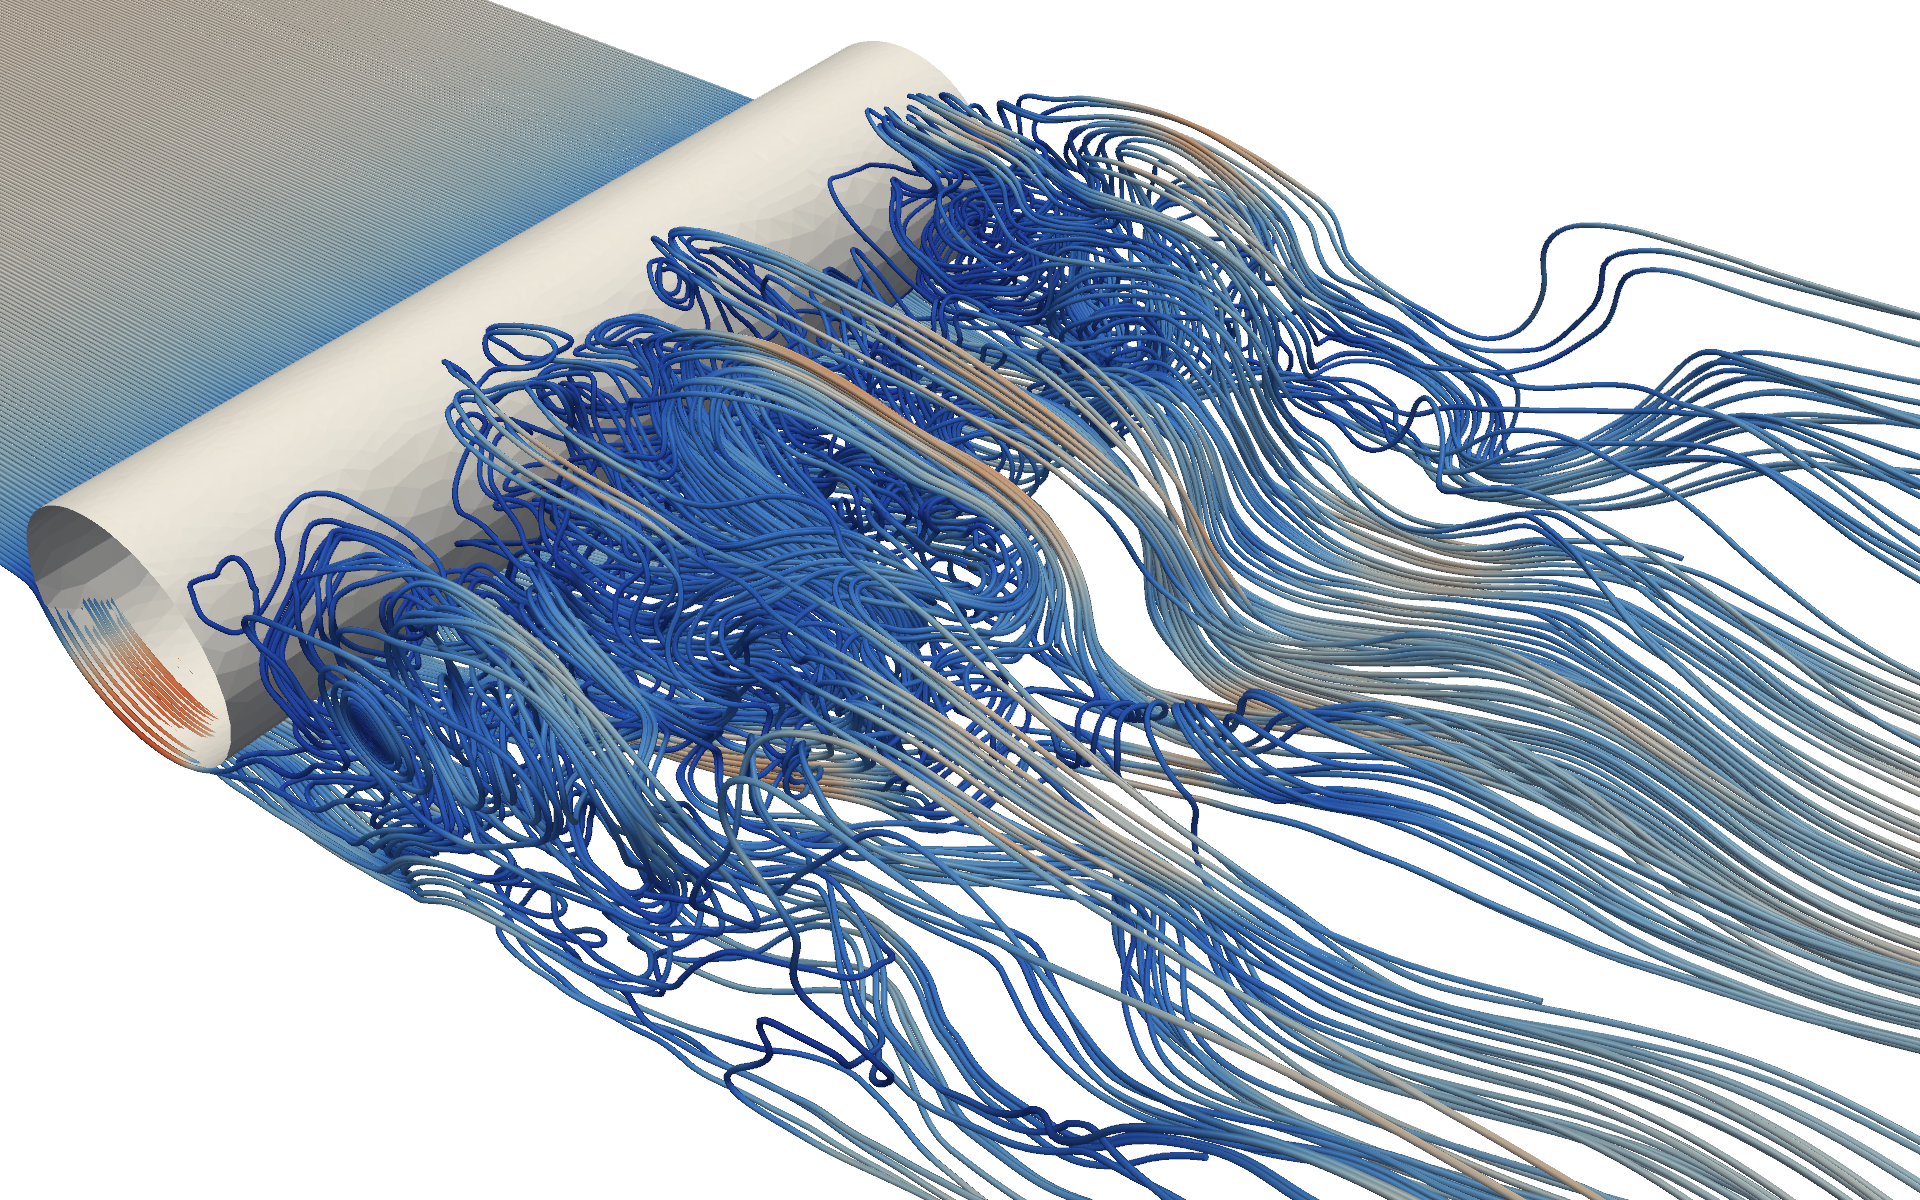
\includegraphics[height=4cm]{unfinished/hoffman-1/png/Hoffman_fig5b.png}
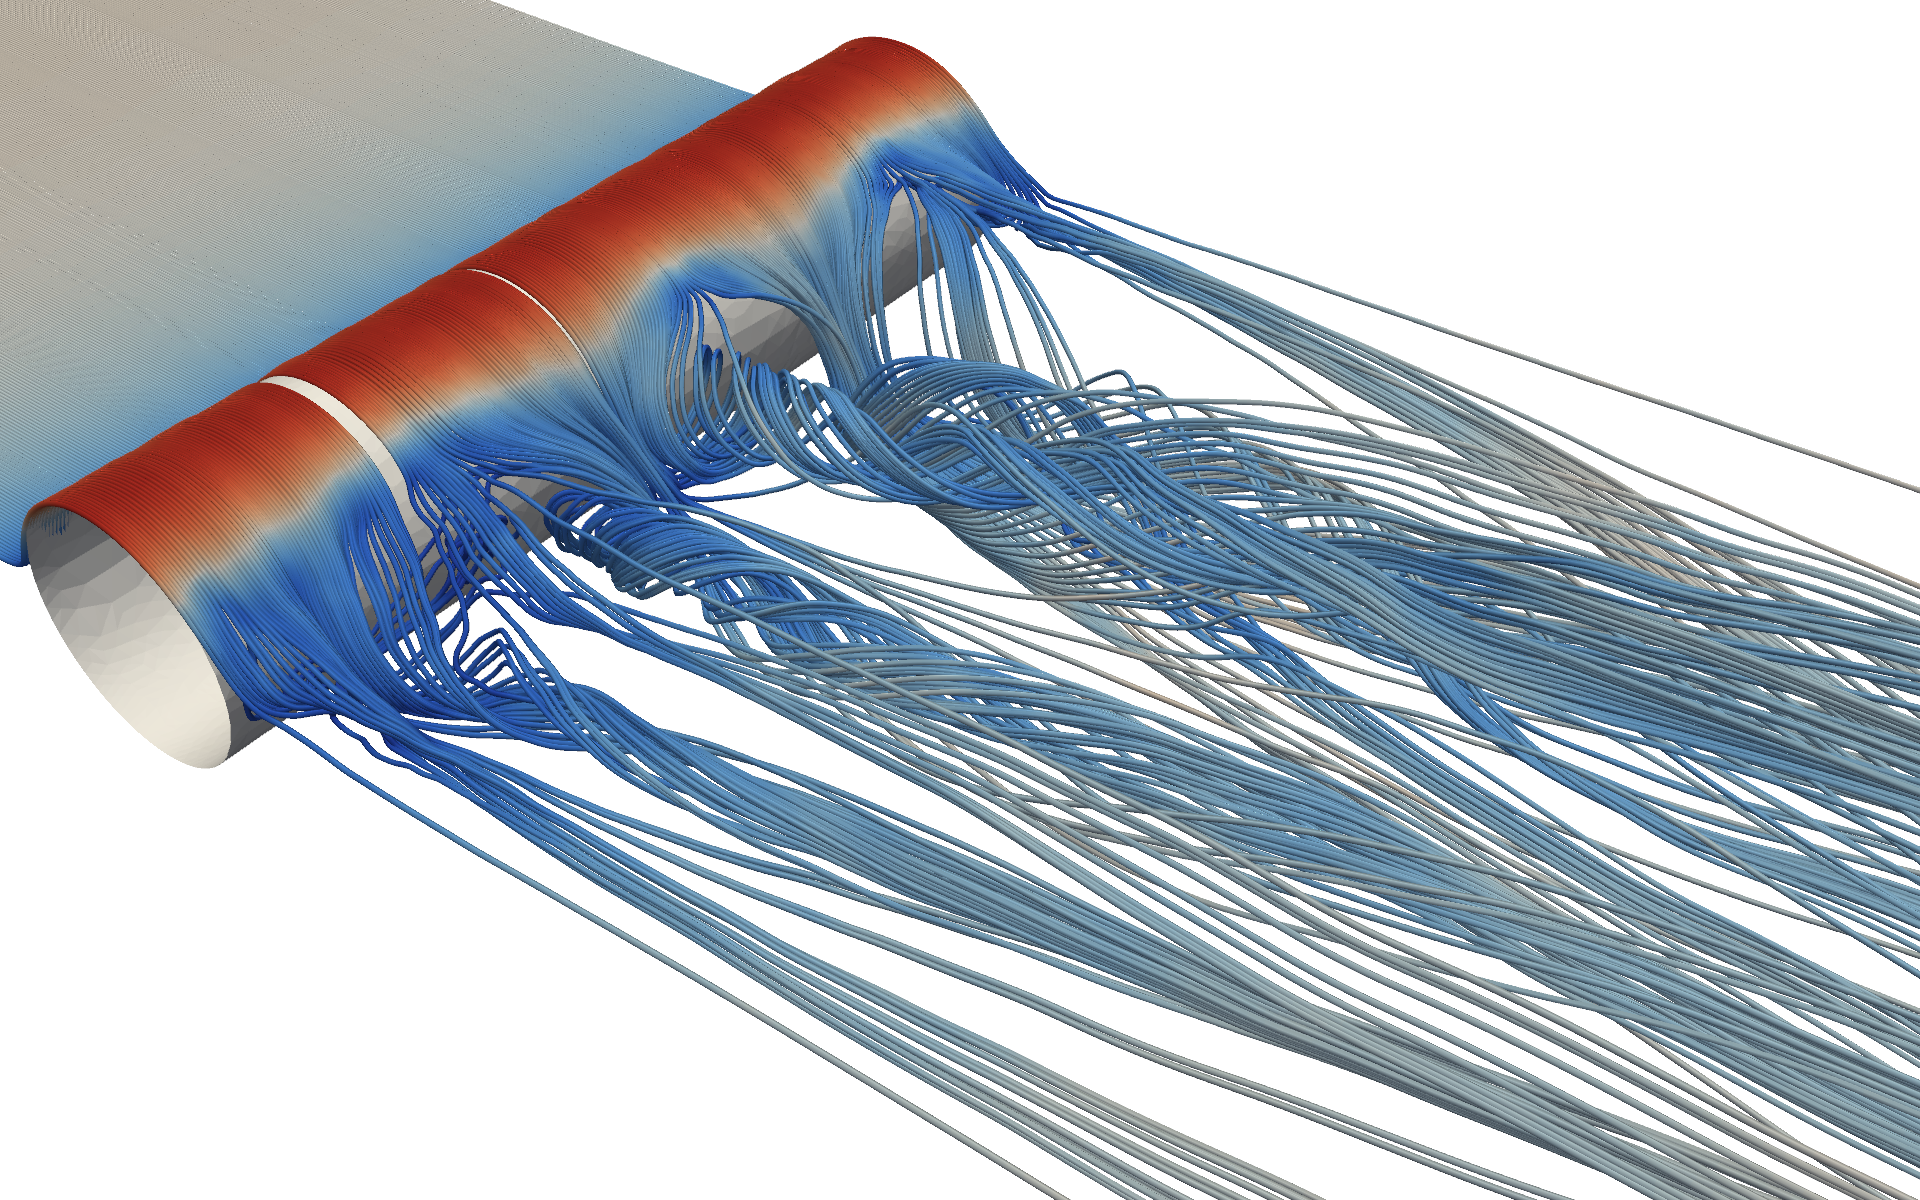
\includegraphics[height=4cm]{unfinished/hoffman-1/png/Hoffman_fig5c.png}
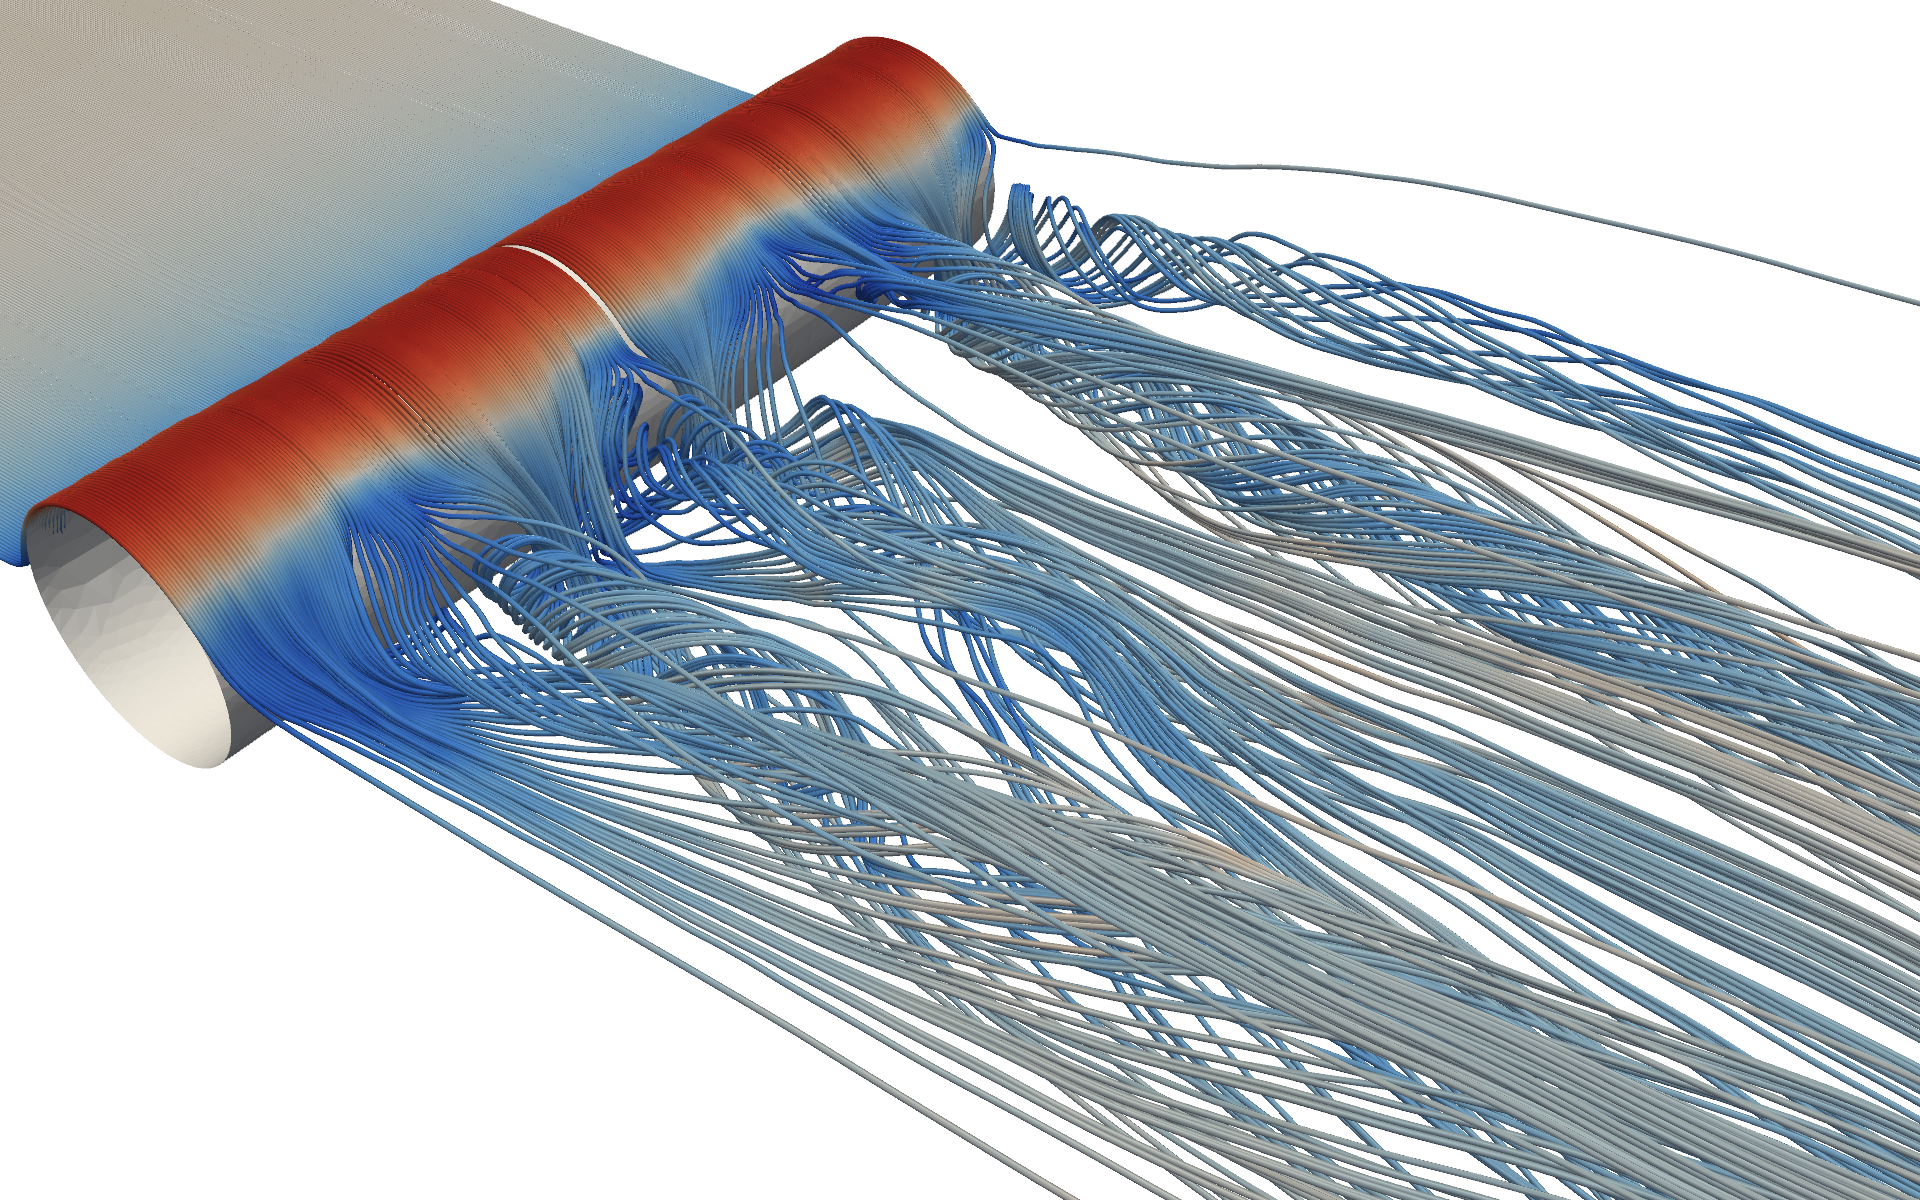
\includegraphics[height=4cm]{unfinished/hoffman-1/png/Hoffman_fig5d.png}
\caption{Turbulent flow separation \cite{HoffmanJansson2009}: velocity streamlines; for $\beta = 10^{-1}$, $\beta = 10^{-2}$, $\beta = 10^{-3}$ and $\beta = 0$ (from upper left to bottom right).}
\label{fig:3}
\end{figure}

\subsection{Turbulent flow past complex geometry}

With the parallel implementation of Unicorn, realistic problems of complex geometry and high Re turbulent flow can be addressed. As an example, we present simulation results from the NASA/AIAA workshop "Benchmark problems for Airframe Noise Computations" (BANC-1), held in conjunction with the 16$^{th}$ AIAA/CEAS Aeroacoustics Conference in Stockholm in 2010, where Unicorn was used for adaptive simulation of flow past a rudimentary landing gear configuration \cite{VilelaJanssonEtAl2010}. The landing gear configuration was designed by Boeing, and detailed experimental results were available, as well as internal comparison within the participating groups \cite{SpalartMejia2011}.

Starting from a coarse mesh of ca 70,000 mesh points, the mesh was adaptively refined 7 times with respect to the error in the drag force on the landing gear. The resulting final mesh had 1,000,000 mesh points, and the computation ran on the \textit{Akka} computer at HPC2N using 264 number of cores. The skin friction boundary layer model was used with $\beta=0$, thus corresponding to a slip boundary condition.

The Unicorn contribution to the workshop compared well with other participating groups, with overall little spread in the computation of aerodynamic forces, and mean sound pressure levels. Also mean flow patterns on the surface of the landing gear (see Fig.\ref{rlg}) showed good agreement with experimental results. Other quantities, such as frequencies, showed a wide spread among the participating groups, and cannot serve as a benchmark test of Unicorn in this setting.

Thanks to the adaptive mesh refinement and the cheap boundary layer model, the Unicorn results were obtained with very few mesh points, less than all other participating groups in the workshop, see Table \ref{tab:hoffman-1-rlg}.

\begin{figure}
\centering
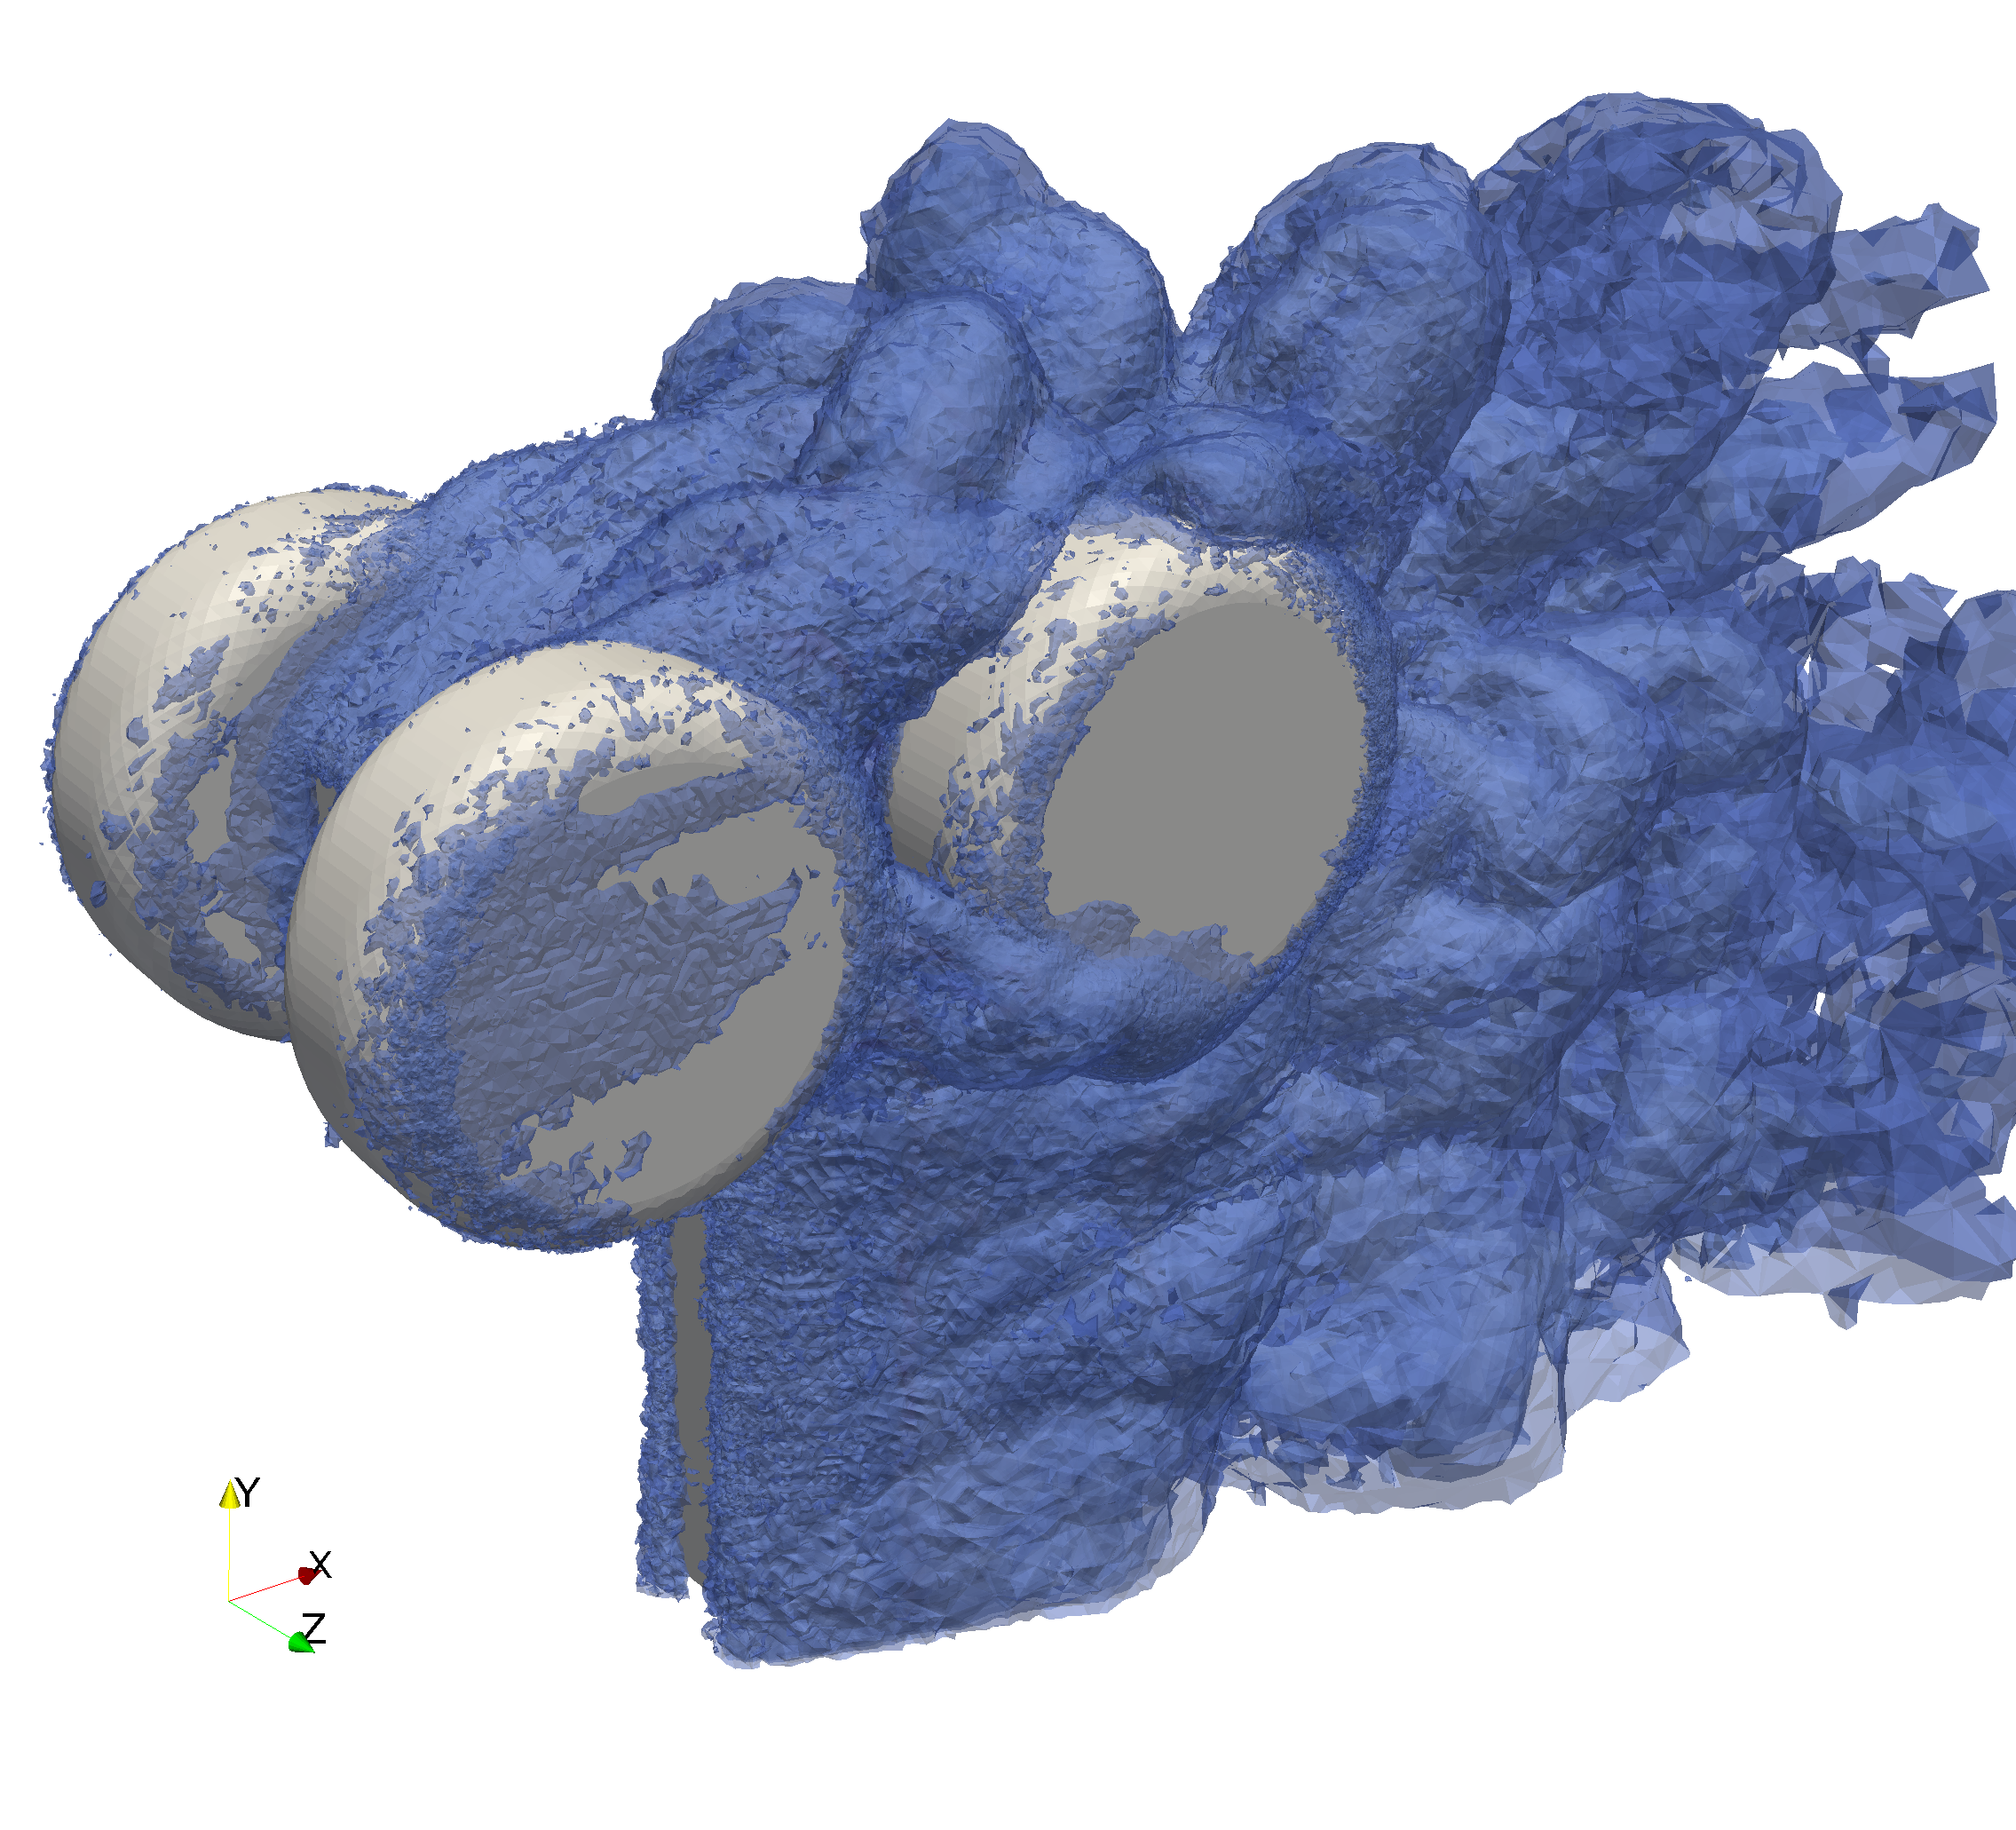
\includegraphics[height=6cm]{unfinished/hoffman-1/png/rlg_vorticity}
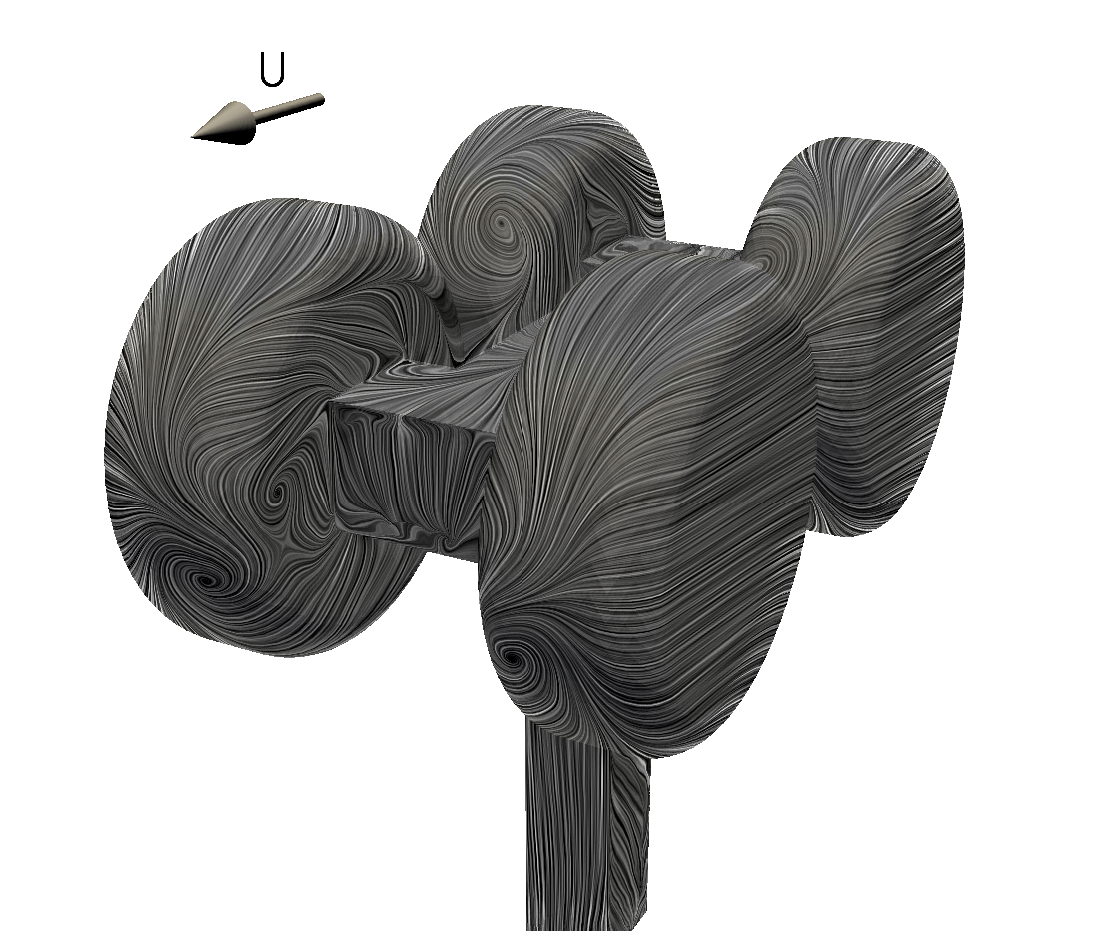
\includegraphics[height=6cm]{unfinished/hoffman-1/png/oilfilm_back_sim}
\caption{Rudimentary landing gear: plot of simulated vorticity (upper) and simulated oil film patterns (lower).}
\label{rlg}
\end{figure}

\begin{table}[hbt]
\begin{center}
\begin{tabular}{|c|cc|}
\hline
Team & $C_D$ & \#Cells \\
\hline
NTS &    1.70 &    10M \\
CDA  &   1.70  &   29M \\
\textbf{KTH}  &   \textbf{1.78}  &   \textbf{6M}\\
KHI  &   1.81  &   41M \\
EXA  &   1.77  &   36M \\
TUB  &   1.74  &   11M \\
\hline
\end{tabular}
\caption{\label{tab:hoffman-1-rlg} Drag coefficient and number of cells for each of the teams in BANC-1 \cite{SpalartMejia2011}. The Unicorn results are the ones by the KTH-team.}
\end{center}
\end{table}

\subsection{Robust fluid-structure interaction}

As a quantitative test of the Unicorn FSI solver we consider the benchmark problem FLUSTRUK-A, variant 3, which is defined in \cite{HronTurek2005}. This is a 2D flow in a channel past a fixed cylinder with a thin flexible bar attached to the downstream side of the cylinder. The Unicorn results are compared to the reference results of 2 other groups: Hron/Turek \cite{HronTurek2005} and Dunne/Rannacher \cite{DunneRannacher2006}.

The y-displacement in the oscillation regime varies between 0.0353m and -0.0332m (see Fig.\ref{fig:flustruk}), which is within 1-2\% of the Hron/Turek results, and within 11\% of the Dunne/Rannacher amplitude. The oscillation frequency is estimated to 5.3Hz from the graph, where the Hron/Turek frequency is estimated to 5.4Hz and the Dunne/Rannacher frequency is given as 5.48 Hz. The Unicorn results are thus within 1-2\% of both groups. See \cite{HoffmanJanssonStockli2011} for a full discussion of the results, where also additional basic benchmark results are presented.

\begin{figure}[!h]
\center{
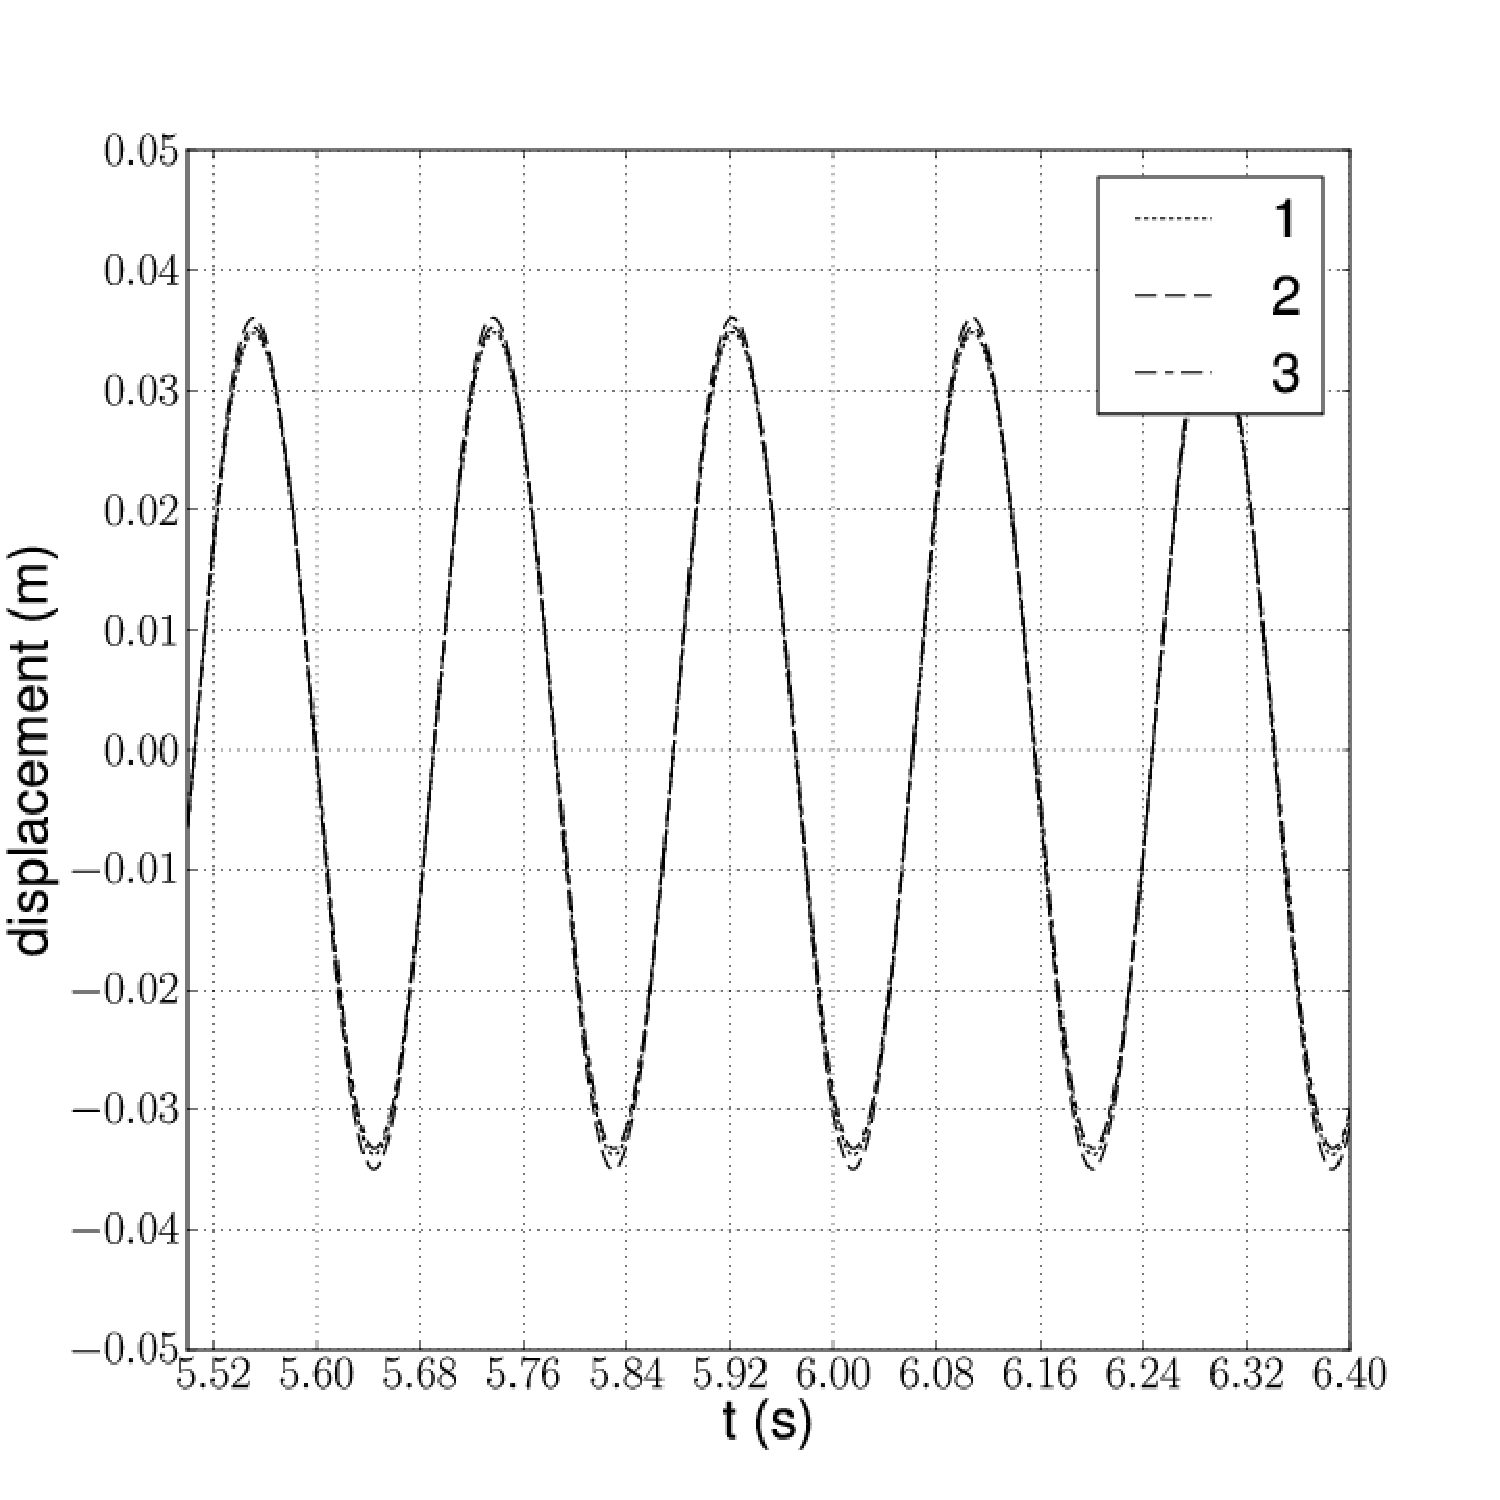
\includegraphics[width=10cm]{unfinished/hoffman-1/png/fsi_bench3D_displacement_aligned.pdf}
}
\caption{
The figure shows the displacement along $y$-axis of the reference point in 2D FSI-benchmark problem FLUSTRUK-A  \cite{HoffmanJanssonStockli2011}, phase aligned to avoid start-up effects, for a sequence of three uniformly refined meshes using Unicorn.
}
\label{fig:flustruk}
\end{figure}

Unicorn target large structure deformations interacting with turbulent fluid flow. In Fig.\ref{fig:flag} we present qualitative results for a model problem of a flexible structure interacting
with turbulent flow in 3D, in the form of a fixed cube in turbulent flow with a thin flexible flag mounted in the downstream wake.

We choose an inflow speed of 1.0e2 m/s, a cube of 1.0e-2 m side and a flag mounted at the top of the back face of the cube with a length of 3.0e-1 m and a thickness of 5.0e-2 m. The viscosity of the fluid of 1.0e-4 Pa s (density $\rho=1$) which gives a representative Reynold's number $Re$ = 1.0e5. We choose no-slip boundary conditions on the cube and flag with slip boundary conditions on the surrounding channel walls, and a zero pressure outflow condition.

Violent bending and torsion motion along the long axis of the flag is observed, and we note that the
method is robust for these large structure deformations and highly fluctuating flow.

\begin{figure}[!h]
\center{
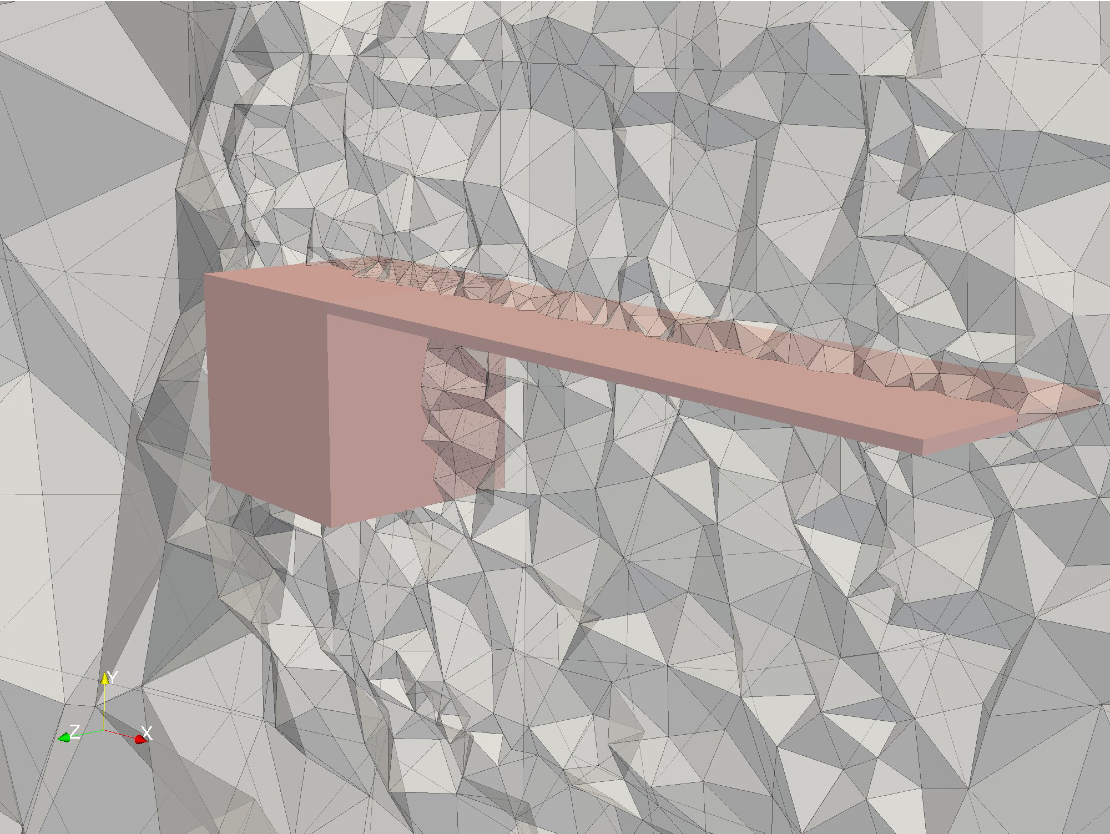
\includegraphics[width=5cm]{unfinished/hoffman-1/png/cube000.png}
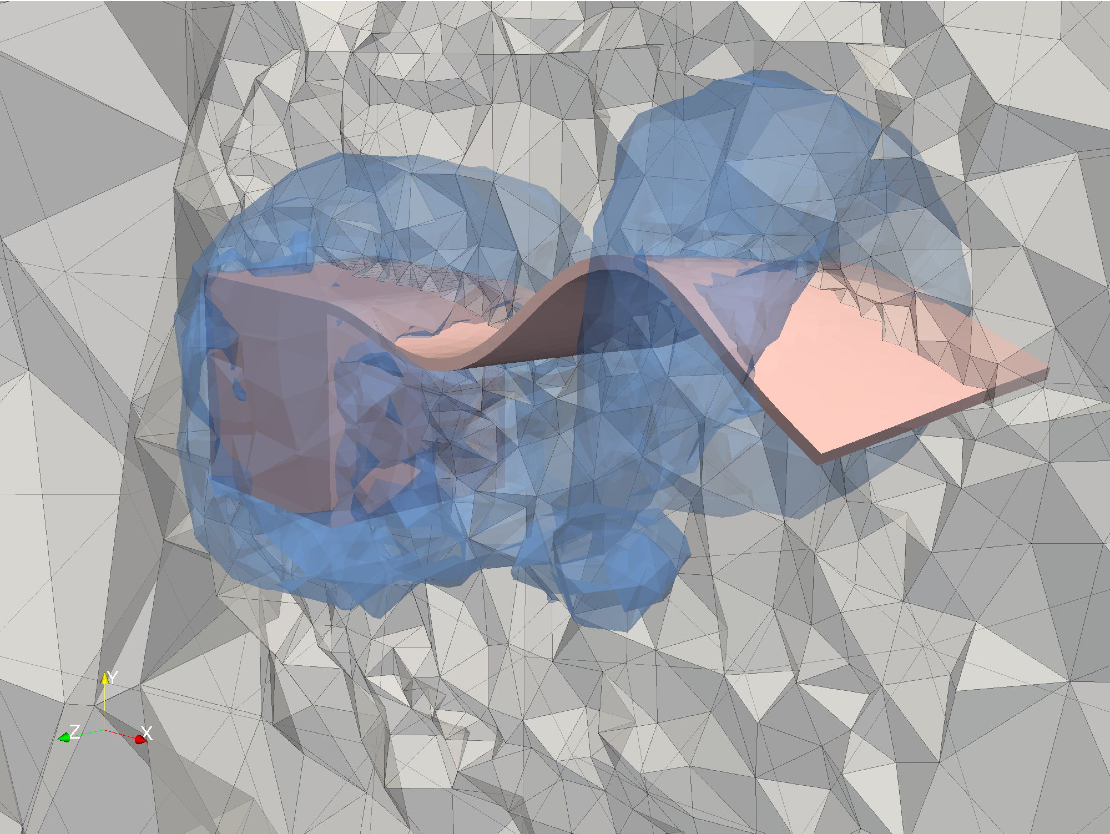
\includegraphics[width=5cm]{unfinished/hoffman-1/png/cube115.png}\\
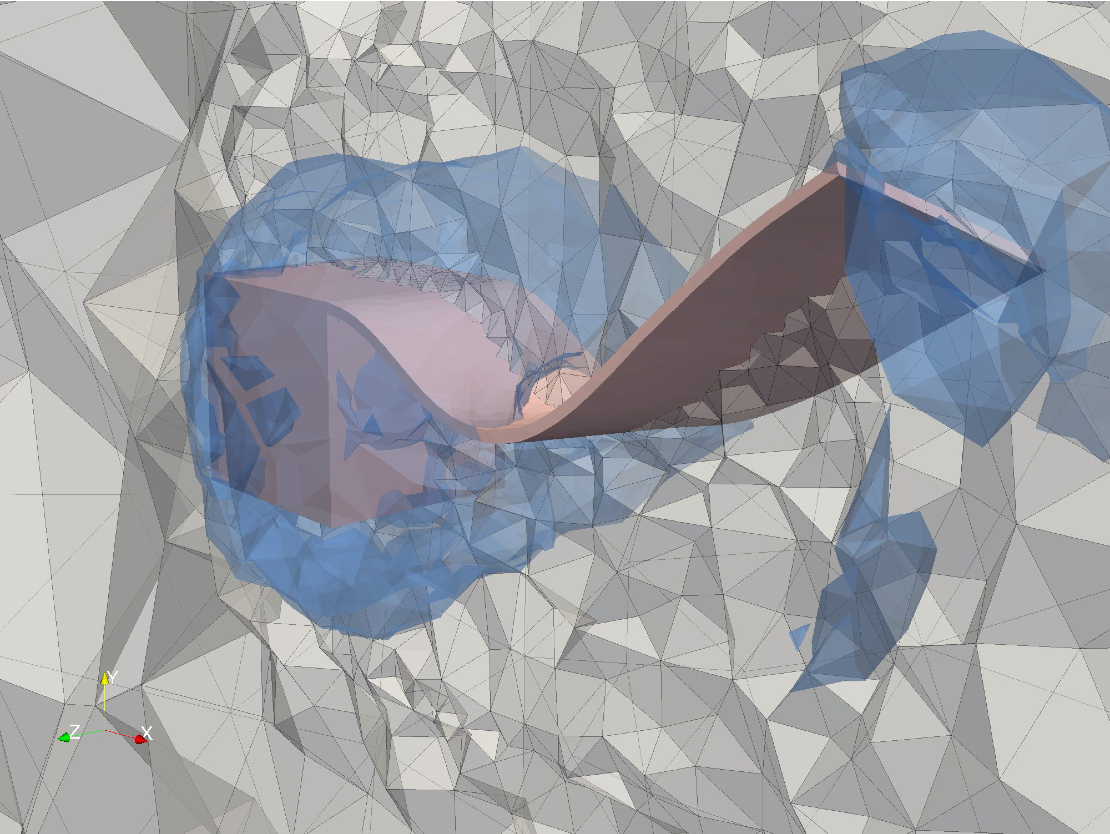
\includegraphics[width=5cm]{unfinished/hoffman-1/png/cube125.png}
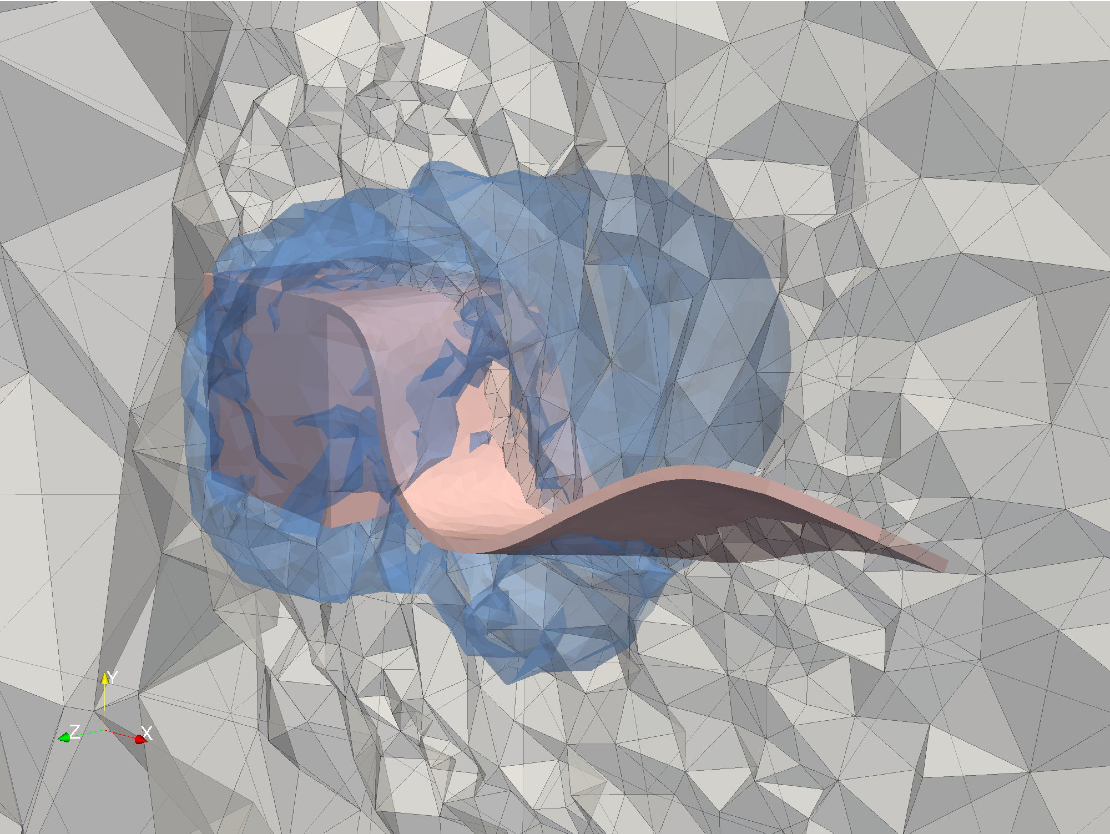
\includegraphics[width=5cm]{unfinished/hoffman-1/png/cube168.png}\\
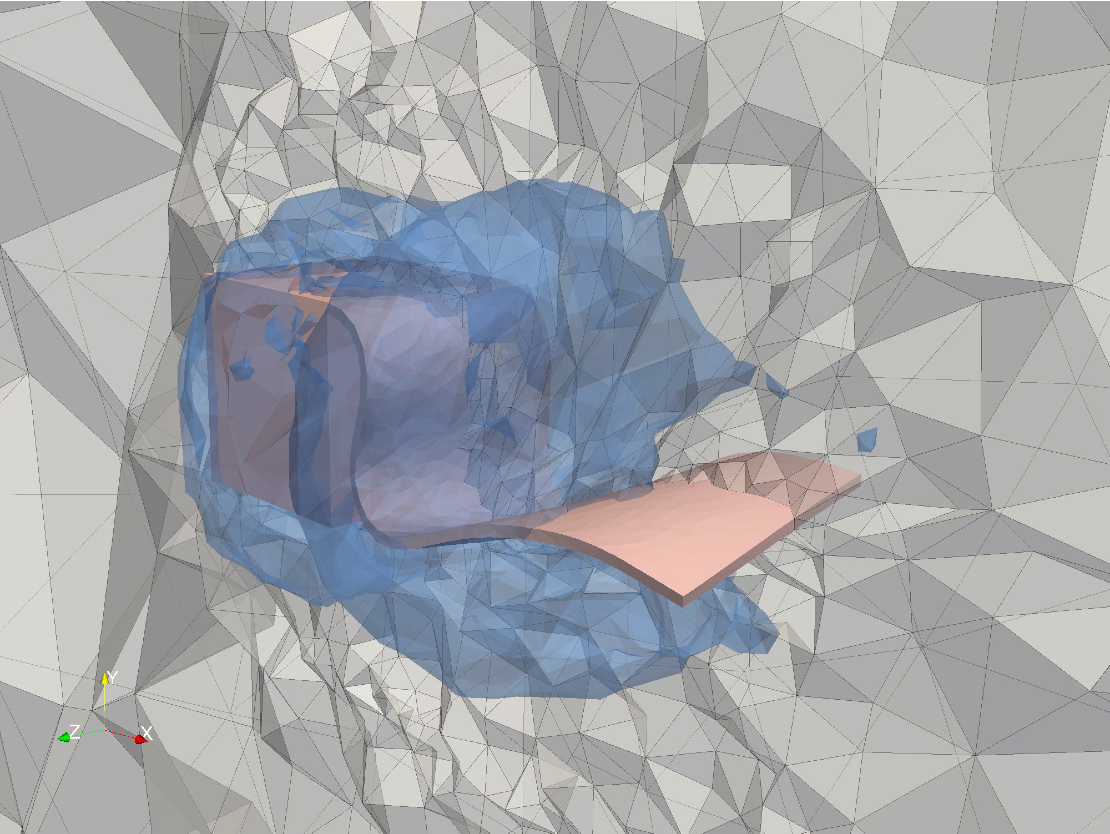
\includegraphics[width=5cm]{unfinished/hoffman-1/png/cube187.png}
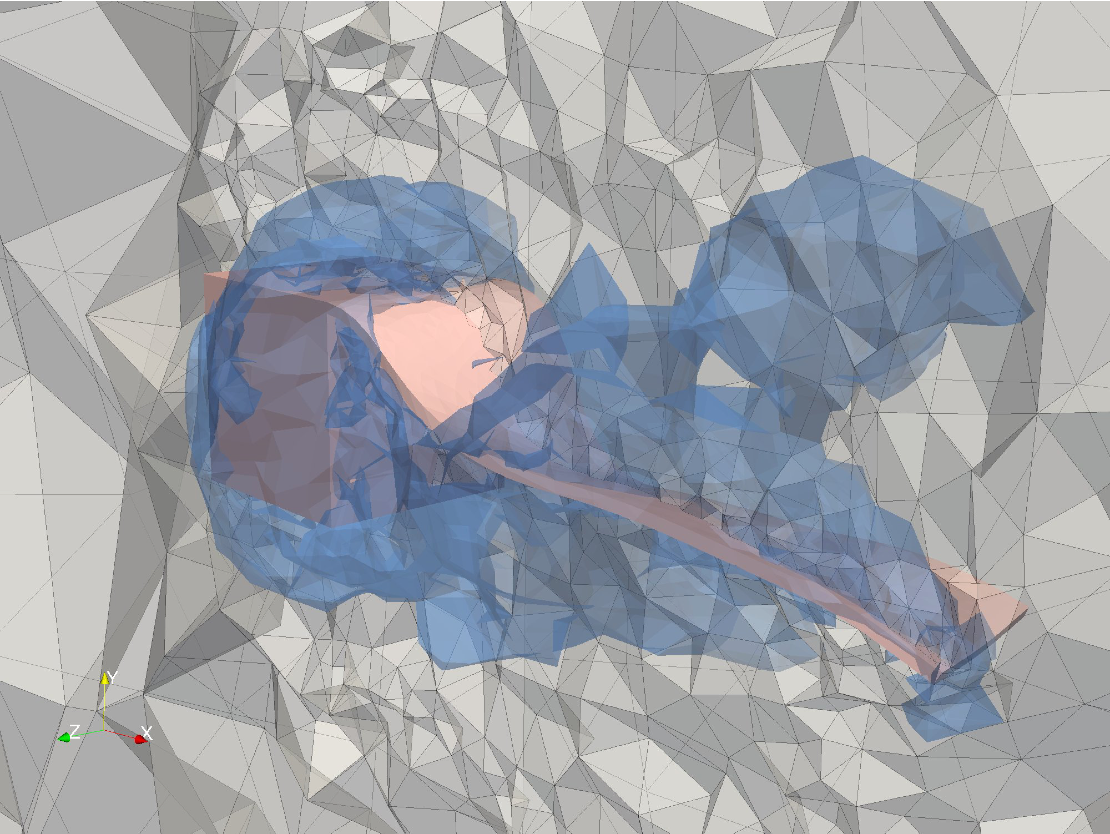
\includegraphics[width=5cm]{unfinished/hoffman-1/png/cube405.png}\\
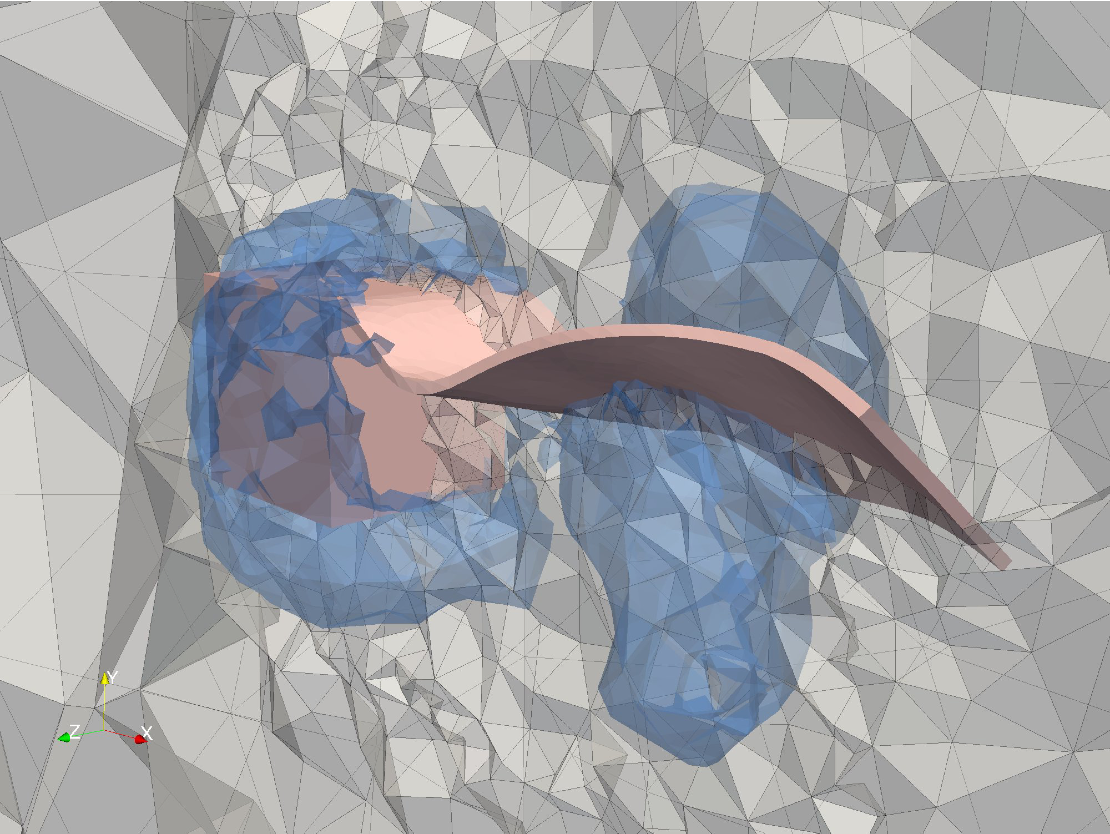
\includegraphics[width=5cm]{unfinished/hoffman-1/png/cube550.png}
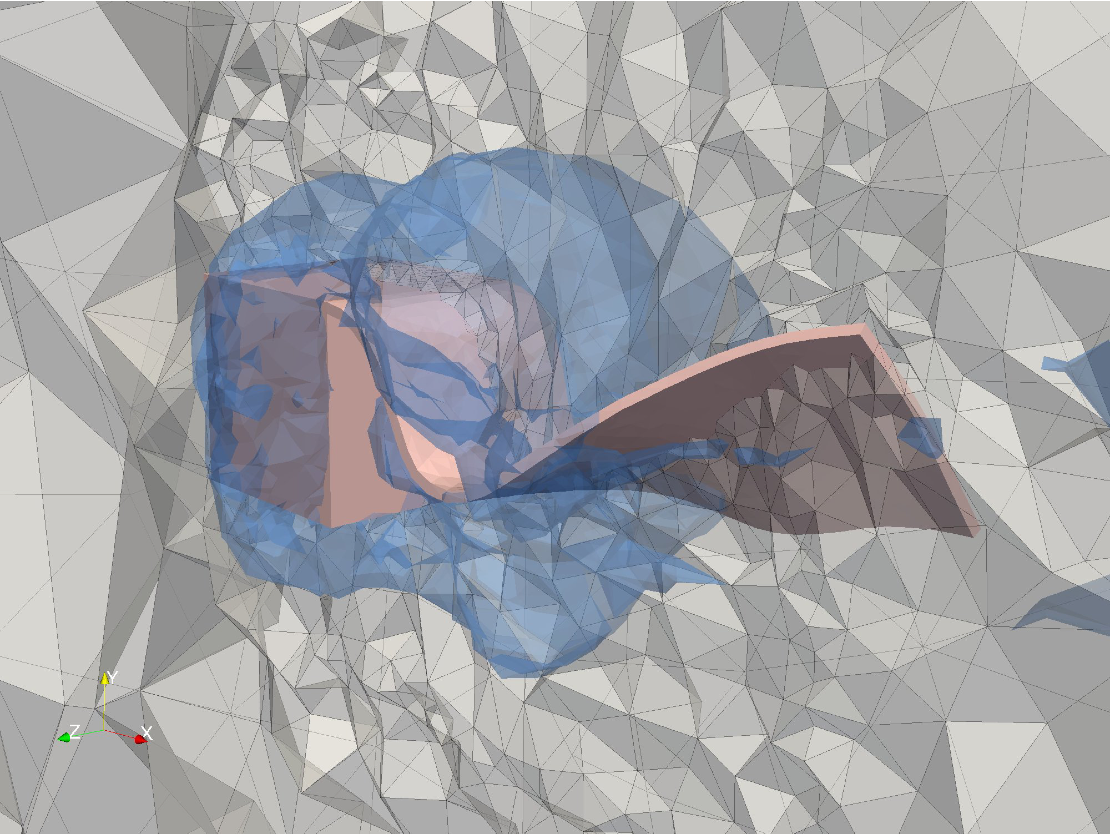
\includegraphics[width=5cm]{unfinished/hoffman-1/png/cube649.png}\\
}
\caption{
Simulation of turbulent flow past a square cylinder with an elastic flag attached downstream \cite{HoffmanJanssonStockli2011}:
plot of cut of the mesh, isosurface of pressure and fluid-structure phase interface. Going from
initial state top left to illustrating violent bending and torsion
motion along the long axis of the flag.
}
\label{fig:flag}
\end{figure}



%%%%\fenicsinput{hoffman-1}
%\fenicsinput{selim}
%%%%\fenicsinput{shan}
%\fenicsinput{lopes}
%\fenicsinput{kvs-2}
%\fenicsinput{hentschel}
%\fenicsinput{narayanan}
%%%%\fenicsinput{oelgaard-1}
%\fenicsinput{nikbakht}
%\fenicsinput{schroll}
%\fenicsinput{hake}
%\fenicsinput{lezar}
\fenicsinput{mardal-4}
%\fenicsinput{rognes}
%
%------------------------------------------------------------------------------
% Start backmatter
\backmatter

% List of authors
\chapter*{List of Authors}

\emph{The following list of authors have contributed to this book.}

\vspace{1cm}

\fenicsauthor{Martin Sandve Aln\ae{}s}{}{}{}{}

\fenicsauthor{Stuart R. Clark}{}{}{}{}

\fenicsauthor{David B. Davidson}
             {davidson@sun.ac.za}
             {Department of Electrical and Electronic Engineering, Stellenbosch University, South Africa}
             {This work is supported by grants from the National Research
              Foundation, South Africa, as well as the Centre for High Performance
              Computing, South Africa as part of a flagship project.}
             {Chapter \ref{chap:lezar}}

\fenicsauthor{Rodrigo Vilela De Abreu}{}{}{}{}

\fenicsauthor{Cem Degirmenci}{}{}{}{}

\fenicsauthor{Johan Hake}{}{}{}{}

\fenicsauthor{Johan Hoffman}{}{}{}{}

\fenicsauthor{Johan Jansson}{}{}{}{}

\fenicsauthor{Niclas Jansson}{}{}{}{}

\fenicsauthor{Claes Johnson}{}{}{}{}

\fenicsauthor{Robert C. Kirby}{}{}{}{}

\fenicsauthor{Matthew G. Knepley}{}{}{}{}

\fenicsauthor{Hans Petter Langtangen}
             {hpl@simula.no}
             {Center for Biomedical Computing at Simula Research Laboratory, Norway \\
              Department of Informatics, University of Oslo, Norway}
             {This work is also supported by a Center of Excellence
              grant from the Research Council of Norway to the Center
              for Biomedical Computing at Simula Research
              Laboratory.}
             {Chapter \ref{chap:langtangen}}

\fenicsauthor{Evan Lezar}
             {mail@evanlezar.com}
             {Department of Electrical and Electronic Engineering, Stellenbosch University, South Africa}
             {This work is supported by grants from the National Research
              Foundation, South Africa, as well as the Centre for High Performance
              Computing, South Africa as part of a flagship project.}
              {Chapter \ref{chap:lezar}}

\fenicsauthor{Svein Linge}{}{}{}{}

\fenicsauthor{Anders Logg}
             {logg@simula.no}
             {Center for Biomedical Computing at Simula Research Laboratory, Norway \\
              Department of Informatics, University of Oslo, Norway}
             {This work is supported by an Outstanding Young
              Investigator grant from the Research Council of Norway,
              NFR 180450. This work is also supported by a Center of
              Excellence grant from the Research Council of Norway to
              the Center for Biomedical Computing at Simula Research
              Laboratory.}
             {Chapters
              \ref{chap:alnes-2}, \ref{chap:kirby-3}, \ref{chap:kirby-4},
              \ref{chap:kirby-5}, \ref{chap:kirby-6}, \ref{chap:kirby-7},
              \ref{chap:kirby-8}, \ref{chap:kvs-1}, \ref{chap:kvs-2},
              \ref{chap:logg-1}, \ref{chap:logg-2}, \ref{chap:logg-3}}

\fenicsauthor{Nuno D. Lopes}{}{}{}{}

\fenicsauthor{Alf Emil L\o{}vgren}{}{}{}{}

\fenicsauthor{Kent-Andre Mardal}
             {kent-and@simula.no}
             {Center for Biomedical Computing at Simula Research Laboratory, Norway \\
              Department of Informatics, University of Oslo, Norway}
             {This work is supported by a Center of Excellence grant
              from the Research Council of Norway to the Center for
              Biomedical Computing at Simula Research Laboratory.}
             {Chapters
              \ref{chap:alnes-1}, \ref{chap:alnes-2}, \ref{chap:alnes-3},
              \ref{chap:hentschel}, \ref{chap:kirby-1}, \ref{chap:kvs-1},
              \ref{chap:kvs-2}, \ref{chap:logg-3}, \ref{chap:mardal-2},
              \ref{chap:mardal-4}, \ref{chap:mortensen}, \ref{chap:wilbers}}

\fenicsauthor{Mikael Mortensen}{}{}{}{}

\fenicsauthor{Harish Narayanan}
             {harish@simula.no}
             {Center for Biomedical Computing at Simula Research Laboratory, Norway}
             {This work is supported by an Outstanding Young
              Investigator grant from the Research Council of Norway,
              NFR 180450. This work is also supported by a Center of
              Excellence grant from the Research Council of Norway to
              the Center for Biomedical Computing at Simula Research
              Laboratory.}
             {Chapters \ref{chap:narayanan} and \ref{chap:kvs-1}}

\fenicsauthor{Murtazo Nazarov}{}{}{}{}

\fenicsauthor{Mehdi Nikbakht}
             {m.nikbakht@tudelft.nl}
             {Faculty of Civil Engineering and Geosciences,
             Delft University of Technology, The Netherlands}
             {Support from the Netherlands Technology Foundation STW,
              the Netherlands Organisation for Scientific Research
              and the Ministry of Public Works and Water Management is
              gratefully acknowledged.}
             {Chapter \ref{chap:nikbakht}}

\fenicsauthor{Pedro Jorge Silva Pereira}{}{}{}{}

\fenicsauthor{Johannes Ring}
             {johannr@simula.no}
             {Center for Biomedical Computing at Simula Research Laboratory, Norway}
             {This work is supported by a Center of Excellence grant
              from the Research Council of Norway to the Center for
              Biomedical Computing at Simula Research Laboratory.}
             {FEniCS packaging, buildbots, benchbots and build system}

\fenicsauthor{Marie E. Rognes}
             {meg@simula.no}
             {Center for Biomedical Computing at Simula Research Laboratory, Norway}
             {This work is supported by an Outstanding Young
              Investigator grant from the Research Council of Norway,
              NFR 180450. This work is also supported by a Center of
              Excellence grant from the Research Council of Norway to
              the Center for Biomedical Computing at Simula Research
              Laboratory.}
             {Chapters
              \ref{chap:logg-1}, \ref{chap:kirby-6}, \ref{chap:rognes}, \ref{chap:vynnytska}}

\fenicsauthor{Hans Joachim Schroll}{}{}{}{}

\fenicsauthor{L. Ridgway Scott}{}{}{}{}

\fenicsauthor{Kristoffer Selim}
             {selim@simula.no}
             {Center for Biomedical Computing at Simula Research Laboratory, Norway}
             {This work is supported by an Outstanding Young
              Investigator grant from the Research Council of Norway,
              NFR 180450. This work is also supported by a Center of
              Excellence grant from the Research Council of Norway to
              the Center for Biomedical Computing at Simula Research
              Laboratory.}
             {Chapter \ref{chap:selim}}

\fenicsauthor{Susanne St\o{}le-Hentschel}{}{}{}{}

\fenicsauthor{Andy R. Terrel}{}{}{}{}

\fenicsauthor{Lu{\'\i}s Trabucho}{}{}{}{}

\fenicsauthor{Kristian Valen-Sendstad}
             {kvs@simula.no}
             {Simula School of Research and Innovation \\
              Center for Biomedical Computing at Simula Research Laboratory, Norway}
             {This work is supported by a Center of Excellence grant
              from the Research Council of Norway to the Center for
              Biomedical Computing at Simula Research Laboratory.}
             {Chapters \ref{chap:kvs-1} and \ref{chap:kvs-1}}

\fenicsauthor{Lyudmyla Vynnytska}{}{}{}{}

\fenicsauthor{Garth N. Wells}
             {gnw20@cam.ac.uk}
             {Department of Enginering, University of Cambridge, United Kingdom}
             {}
             {}

\fenicsauthor{Ilmar M. Wilbers}{}{}{}{}

\fenicsauthor{Kristian B. \O{}lgaard}{}{}{}{}


% Bibliography
\bibliography{bibliography}
\bibliographystyle{abbrvnat}

% End full width
\end{fullwidth}

% Index
%\newcommand{\icode}[1]{\texttt{#1}} % seems necessary
%\printindex
%------------------------------------------------------------------------------
\end{document}
%------------------------------------------------------------------------------
